\documentclass[twoside]{book}

% Packages required by doxygen
\usepackage{calc}
\usepackage{doxygen}
\usepackage{graphicx}
\usepackage[utf8]{inputenc}
\usepackage{makeidx}
\usepackage{multicol}
\usepackage{multirow}
\usepackage{textcomp}
\usepackage[table]{xcolor}

% Font selection
\usepackage[T1]{fontenc}
\usepackage{mathptmx}
\usepackage[scaled=.90]{helvet}
\usepackage{courier}
\usepackage{amssymb}
\usepackage{sectsty}
\renewcommand{\familydefault}{\sfdefault}
\allsectionsfont{%
  \fontseries{bc}\selectfont%
  \color{darkgray}%
}
\renewcommand{\DoxyLabelFont}{%
  \fontseries{bc}\selectfont%
  \color{darkgray}%
}

% Page & text layout
\usepackage{geometry}
\geometry{%
  a4paper,%
  top=2.5cm,%
  bottom=2.5cm,%
  left=2.5cm,%
  right=2.5cm%
}
\tolerance=750
\hfuzz=15pt
\hbadness=750
\setlength{\emergencystretch}{15pt}
\setlength{\parindent}{0cm}
\setlength{\parskip}{0.2cm}
\makeatletter
\renewcommand{\paragraph}{%
  \@startsection{paragraph}{4}{0ex}{-1.0ex}{1.0ex}{%
    \normalfont\normalsize\bfseries\SS@parafont%
  }%
}
\renewcommand{\subparagraph}{%
  \@startsection{subparagraph}{5}{0ex}{-1.0ex}{1.0ex}{%
    \normalfont\normalsize\bfseries\SS@subparafont%
  }%
}
\makeatother

% Headers & footers
\usepackage{fancyhdr}
\pagestyle{fancyplain}
\fancyhead[LE]{\fancyplain{}{\bfseries\thepage}}
\fancyhead[CE]{\fancyplain{}{}}
\fancyhead[RE]{\fancyplain{}{\bfseries\leftmark}}
\fancyhead[LO]{\fancyplain{}{\bfseries\rightmark}}
\fancyhead[CO]{\fancyplain{}{}}
\fancyhead[RO]{\fancyplain{}{\bfseries\thepage}}
\fancyfoot[LE]{\fancyplain{}{}}
\fancyfoot[CE]{\fancyplain{}{}}
\fancyfoot[RE]{\fancyplain{}{\bfseries\scriptsize 生成于 2013年 八月 12日 星期一 15:24:04 , 为 VirtualDiskConsole使用  Doxygen }}
\fancyfoot[LO]{\fancyplain{}{\bfseries\scriptsize 生成于 2013年 八月 12日 星期一 15:24:04 , 为 VirtualDiskConsole使用  Doxygen }}
\fancyfoot[CO]{\fancyplain{}{}}
\fancyfoot[RO]{\fancyplain{}{}}
\renewcommand{\footrulewidth}{0.4pt}
\renewcommand{\chaptermark}[1]{%
  \markboth{#1}{}%
}
\renewcommand{\sectionmark}[1]{%
  \markright{\thesection\ #1}%
}

% Indices & bibliography
\usepackage{natbib}
\usepackage[titles]{tocloft}
\setcounter{tocdepth}{3}
\setcounter{secnumdepth}{5}
\makeindex

% Hyperlinks (required, but should be loaded last)
\usepackage{ifpdf}
\ifpdf
  \usepackage[pdftex,pagebackref=true]{hyperref}
\else
  \usepackage[ps2pdf,pagebackref=true]{hyperref}
\fi
\hypersetup{%
  colorlinks=true,%
  linkcolor=blue,%
  citecolor=blue,%
  unicode%
}

% Custom commands
\newcommand{\clearemptydoublepage}{%
  \newpage{\pagestyle{empty}\cleardoublepage}%
}


%===== C O N T E N T S =====

\begin{document}

% Titlepage & ToC
\hypersetup{pageanchor=false}
\pagenumbering{roman}
\begin{titlepage}
\vspace*{7cm}
\begin{center}%
{\Large Virtual\-Disk\-Console }\\
\vspace*{1cm}
{\large 制作者 Doxygen 1.8.4}\\
\vspace*{0.5cm}
{\small 2013年 八月 12日 星期一 15:24:04}\\
\end{center}
\end{titlepage}
\clearemptydoublepage
\tableofcontents
\clearemptydoublepage
\pagenumbering{arabic}
\hypersetup{pageanchor=true}

%--- Begin generated contents ---
\chapter{命名空间索引}
\section{命名空间列表}
这里列出了所有文档化的命名空间定义,附带简要说明\-:\begin{DoxyCompactList}
\item\contentsline{section}{\hyperlink{namespace_lexer_sys}{Lexer\-Sys} }{\pageref{namespace_lexer_sys}}{}
\end{DoxyCompactList}

\chapter{继承关系索引}
\section{类继承关系}
此继承关系列表按字典顺序粗略的排序\-: \begin{DoxyCompactList}
\item \contentsline{section}{Command\-Sys\-:\-:Console\-Command}{\pageref{class_command_sys_1_1_console_command}}{}
\begin{DoxyCompactList}
\item \contentsline{section}{Command\-Sys\-:\-:Cd\-Cmd}{\pageref{class_command_sys_1_1_cd_cmd}}{}
\item \contentsline{section}{Command\-Sys\-:\-:Compare\-Cmd}{\pageref{class_command_sys_1_1_compare_cmd}}{}
\item \contentsline{section}{Command\-Sys\-:\-:Copy\-Cmd}{\pageref{class_command_sys_1_1_copy_cmd}}{}
\item \contentsline{section}{Command\-Sys\-:\-:Del\-Cmd}{\pageref{class_command_sys_1_1_del_cmd}}{}
\item \contentsline{section}{Command\-Sys\-:\-:Dir\-Cmd}{\pageref{class_command_sys_1_1_dir_cmd}}{}
\item \contentsline{section}{Command\-Sys\-:\-:Mkdir\-Cmd}{\pageref{class_command_sys_1_1_mkdir_cmd}}{}
\item \contentsline{section}{Command\-Sys\-:\-:Rmdir\-Cmd}{\pageref{class_command_sys_1_1_rmdir_cmd}}{}
\end{DoxyCompactList}
\item \contentsline{section}{Util\-:\-:Link\-List\-T$<$ T $>$\-:\-:Iterator}{\pageref{class_util_1_1_link_list_t_1_1_iterator}}{}
\item \contentsline{section}{Lexer\-Sys\-:\-:Lexer}{\pageref{class_lexer_sys_1_1_lexer}}{}
\item \contentsline{section}{Util\-:\-:Link\-List\-T$<$ T $>$}{\pageref{class_util_1_1_link_list_t}}{}
\item \contentsline{section}{Util\-:\-:Link\-List\-T$<$ File\-Sys\-:\-:Node $\ast$ $>$}{\pageref{class_util_1_1_link_list_t}}{}
\item \contentsline{section}{Util\-:\-:Link\-List\-T$<$ Lexer\-Sys\-:\-:Search\-Path $>$}{\pageref{class_util_1_1_link_list_t}}{}
\item \contentsline{section}{Util\-:\-:Link\-List\-T$<$ Lexer\-Sys\-:\-:Token $>$}{\pageref{class_util_1_1_link_list_t}}{}
\item \contentsline{section}{Util\-:\-:Link\-List\-T$<$ Token $>$}{\pageref{class_util_1_1_link_list_t}}{}
\item \contentsline{section}{Util\-:\-:Link\-List\-T$<$ Util\-:\-:String $>$}{\pageref{class_util_1_1_link_list_t}}{}
\item \contentsline{section}{Util\-:\-:Link\-List\-T$<$ T $>$\-:\-:Link\-Node}{\pageref{class_util_1_1_link_list_t_1_1_link_node}}{}
\item \contentsline{section}{File\-Sys\-:\-:Node}{\pageref{class_file_sys_1_1_node}}{}
\begin{DoxyCompactList}
\item \contentsline{section}{File\-Sys\-:\-:File\-Node}{\pageref{class_file_sys_1_1_file_node}}{}
\item \contentsline{section}{File\-Sys\-:\-:Folder\-Node}{\pageref{class_file_sys_1_1_folder_node}}{}
\end{DoxyCompactList}
\item \contentsline{section}{File\-Sys\-:\-:Node\-Visitor}{\pageref{class_file_sys_1_1_node_visitor}}{}
\begin{DoxyCompactList}
\item \contentsline{section}{File\-Sys\-:\-:Create\-Dir\-Visitor}{\pageref{class_file_sys_1_1_create_dir_visitor}}{}
\item \contentsline{section}{File\-Sys\-:\-:Path\-Search\-Visitor}{\pageref{class_file_sys_1_1_path_search_visitor}}{}
\end{DoxyCompactList}
\item \contentsline{section}{Util\-:\-:Queue\-T$<$ T $>$}{\pageref{class_util_1_1_queue_t}}{}
\item \contentsline{section}{Util\-:\-:Queue\-T$<$ Util\-:\-:String $>$}{\pageref{class_util_1_1_queue_t}}{}
\item \contentsline{section}{Lexer\-Sys\-:\-:Search\-Path}{\pageref{class_lexer_sys_1_1_search_path}}{}
\item \contentsline{section}{Util\-:\-:Singleton\-T$<$ T $>$}{\pageref{class_util_1_1_singleton_t}}{}
\item \contentsline{section}{Util\-:\-:Singleton\-T$<$ Console\-Command\-Factory $>$}{\pageref{class_util_1_1_singleton_t}}{}
\begin{DoxyCompactList}
\item \contentsline{section}{Command\-Sys\-:\-:Console\-Command\-Factory}{\pageref{class_command_sys_1_1_console_command_factory}}{}
\end{DoxyCompactList}
\item \contentsline{section}{Util\-:\-:Singleton\-T$<$ File\-System $>$}{\pageref{class_util_1_1_singleton_t}}{}
\begin{DoxyCompactList}
\item \contentsline{section}{File\-Sys\-:\-:File\-System}{\pageref{class_file_sys_1_1_file_system}}{}
\end{DoxyCompactList}
\item \contentsline{section}{Util\-:\-:Singleton\-T$<$ Virtual\-Disk\-Console $>$}{\pageref{class_util_1_1_singleton_t}}{}
\begin{DoxyCompactList}
\item \contentsline{section}{Virtual\-Disk\-Console}{\pageref{class_virtual_disk_console}}{}
\end{DoxyCompactList}
\item \contentsline{section}{Util\-:\-:Stack\-T$<$ T $>$}{\pageref{class_util_1_1_stack_t}}{}
\item \contentsline{section}{Util\-:\-:String\-T$<$ T $>$}{\pageref{class_util_1_1_string_t}}{}
\item \contentsline{section}{Lexer\-Sys\-:\-:Token}{\pageref{class_lexer_sys_1_1_token}}{}
\item \contentsline{section}{Util\-:\-:Vector\-T$<$ T $>$}{\pageref{class_util_1_1_vector_t}}{}
\end{DoxyCompactList}

\chapter{类索引}
\section{类列表}
这里列出了所有类、结构、联合以及接口定义等,并附带简要说明\-:\begin{DoxyCompactList}
\item\contentsline{section}{\hyperlink{class_command_sys_1_1_cd_cmd}{Command\-Sys\-::\-Cd\-Cmd} }{\pageref{class_command_sys_1_1_cd_cmd}}{}
\item\contentsline{section}{\hyperlink{class_command_sys_1_1_compare_cmd}{Command\-Sys\-::\-Compare\-Cmd} }{\pageref{class_command_sys_1_1_compare_cmd}}{}
\item\contentsline{section}{\hyperlink{class_command_sys_1_1_console_command}{Command\-Sys\-::\-Console\-Command} }{\pageref{class_command_sys_1_1_console_command}}{}
\item\contentsline{section}{\hyperlink{class_command_sys_1_1_console_command_factory}{Command\-Sys\-::\-Console\-Command\-Factory} }{\pageref{class_command_sys_1_1_console_command_factory}}{}
\item\contentsline{section}{\hyperlink{class_command_sys_1_1_copy_cmd}{Command\-Sys\-::\-Copy\-Cmd} }{\pageref{class_command_sys_1_1_copy_cmd}}{}
\item\contentsline{section}{\hyperlink{class_file_sys_1_1_create_dir_visitor}{File\-Sys\-::\-Create\-Dir\-Visitor} }{\pageref{class_file_sys_1_1_create_dir_visitor}}{}
\item\contentsline{section}{\hyperlink{class_command_sys_1_1_del_cmd}{Command\-Sys\-::\-Del\-Cmd} }{\pageref{class_command_sys_1_1_del_cmd}}{}
\item\contentsline{section}{\hyperlink{class_command_sys_1_1_dir_cmd}{Command\-Sys\-::\-Dir\-Cmd} }{\pageref{class_command_sys_1_1_dir_cmd}}{}
\item\contentsline{section}{\hyperlink{class_file_sys_1_1_file_node}{File\-Sys\-::\-File\-Node} }{\pageref{class_file_sys_1_1_file_node}}{}
\item\contentsline{section}{\hyperlink{class_file_sys_1_1_file_system}{File\-Sys\-::\-File\-System} }{\pageref{class_file_sys_1_1_file_system}}{}
\item\contentsline{section}{\hyperlink{class_file_sys_1_1_folder_node}{File\-Sys\-::\-Folder\-Node} }{\pageref{class_file_sys_1_1_folder_node}}{}
\item\contentsline{section}{\hyperlink{class_util_1_1_link_list_t_1_1_iterator}{Util\-::\-Link\-List\-T$<$ T $>$\-::\-Iterator} }{\pageref{class_util_1_1_link_list_t_1_1_iterator}}{}
\item\contentsline{section}{\hyperlink{class_lexer_sys_1_1_lexer}{Lexer\-Sys\-::\-Lexer} }{\pageref{class_lexer_sys_1_1_lexer}}{}
\item\contentsline{section}{\hyperlink{class_util_1_1_link_list_t}{Util\-::\-Link\-List\-T$<$ T $>$} }{\pageref{class_util_1_1_link_list_t}}{}
\item\contentsline{section}{\hyperlink{class_util_1_1_link_list_t_1_1_link_node}{Util\-::\-Link\-List\-T$<$ T $>$\-::\-Link\-Node} }{\pageref{class_util_1_1_link_list_t_1_1_link_node}}{}
\item\contentsline{section}{\hyperlink{class_command_sys_1_1_mkdir_cmd}{Command\-Sys\-::\-Mkdir\-Cmd} }{\pageref{class_command_sys_1_1_mkdir_cmd}}{}
\item\contentsline{section}{\hyperlink{class_file_sys_1_1_node}{File\-Sys\-::\-Node} }{\pageref{class_file_sys_1_1_node}}{}
\item\contentsline{section}{\hyperlink{class_file_sys_1_1_node_visitor}{File\-Sys\-::\-Node\-Visitor} }{\pageref{class_file_sys_1_1_node_visitor}}{}
\item\contentsline{section}{\hyperlink{class_file_sys_1_1_path_search_visitor}{File\-Sys\-::\-Path\-Search\-Visitor} }{\pageref{class_file_sys_1_1_path_search_visitor}}{}
\item\contentsline{section}{\hyperlink{class_util_1_1_queue_t}{Util\-::\-Queue\-T$<$ T $>$} }{\pageref{class_util_1_1_queue_t}}{}
\item\contentsline{section}{\hyperlink{class_command_sys_1_1_rmdir_cmd}{Command\-Sys\-::\-Rmdir\-Cmd} }{\pageref{class_command_sys_1_1_rmdir_cmd}}{}
\item\contentsline{section}{\hyperlink{class_lexer_sys_1_1_search_path}{Lexer\-Sys\-::\-Search\-Path} }{\pageref{class_lexer_sys_1_1_search_path}}{}
\item\contentsline{section}{\hyperlink{class_util_1_1_singleton_t}{Util\-::\-Singleton\-T$<$ T $>$} }{\pageref{class_util_1_1_singleton_t}}{}
\item\contentsline{section}{\hyperlink{class_util_1_1_stack_t}{Util\-::\-Stack\-T$<$ T $>$} }{\pageref{class_util_1_1_stack_t}}{}
\item\contentsline{section}{\hyperlink{class_util_1_1_string_t}{Util\-::\-String\-T$<$ T $>$} }{\pageref{class_util_1_1_string_t}}{}
\item\contentsline{section}{\hyperlink{class_lexer_sys_1_1_token}{Lexer\-Sys\-::\-Token} }{\pageref{class_lexer_sys_1_1_token}}{}
\item\contentsline{section}{\hyperlink{class_util_1_1_vector_t}{Util\-::\-Vector\-T$<$ T $>$} }{\pageref{class_util_1_1_vector_t}}{}
\item\contentsline{section}{\hyperlink{class_virtual_disk_console}{Virtual\-Disk\-Console} }{\pageref{class_virtual_disk_console}}{}
\end{DoxyCompactList}

\chapter{命名空间文档}
\hypertarget{namespace_lexer_sys}{\section{Lexer\-Sys 命名空间参考}
\label{namespace_lexer_sys}\index{Lexer\-Sys@{Lexer\-Sys}}
}
\subsection*{类}
\begin{DoxyCompactItemize}
\item 
class \hyperlink{class_lexer_sys_1_1_lexer}{Lexer}
\item 
class \hyperlink{class_lexer_sys_1_1_search_path}{Search\-Path}
\item 
class \hyperlink{class_lexer_sys_1_1_token}{Token}
\end{DoxyCompactItemize}
\subsection*{变量}
\begin{DoxyCompactItemize}
\item 
\hypertarget{namespace_lexer_sys_adbbadc36e46ed4eee23ccd26993e0c49}{const int {\bfseries P\-A\-T\-H\-\_\-\-L\-E\-N\-G\-T\-H\-\_\-\-L\-I\-M\-I\-T} = 256}\label{namespace_lexer_sys_adbbadc36e46ed4eee23ccd26993e0c49}

\end{DoxyCompactItemize}


\subsection{详细描述}
\begin{DoxyAuthor}{作者}
zhangpeng 
\end{DoxyAuthor}
\begin{DoxyVersion}{版本}
1.\-0  06-\/八月-\/2013 9\-:17\-:33 
\end{DoxyVersion}

\chapter{类说明}
\hypertarget{class_command_sys_1_1_cd_cmd}{\section{Command\-Sys\-:\-:Cd\-Cmd类 参考}
\label{class_command_sys_1_1_cd_cmd}\index{Command\-Sys\-::\-Cd\-Cmd@{Command\-Sys\-::\-Cd\-Cmd}}
}
类 Command\-Sys\-:\-:Cd\-Cmd 继承关系图\-:\begin{figure}[H]
\begin{center}
\leavevmode
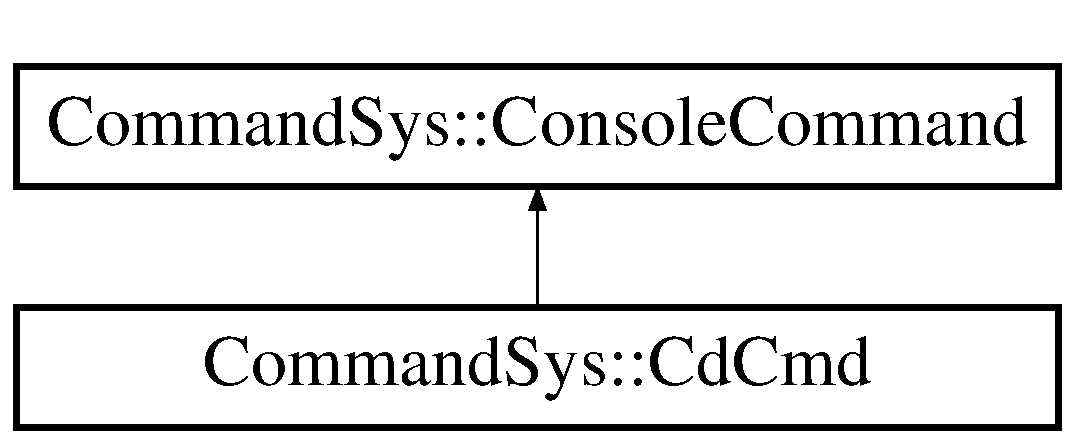
\includegraphics[height=2.000000cm]{class_command_sys_1_1_cd_cmd}
\end{center}
\end{figure}
\subsection*{Public 成员函数}
\begin{DoxyCompactItemize}
\item 
virtual void \hyperlink{class_command_sys_1_1_cd_cmd_af355386817b6cad86d370d65267d5d88}{Execute} (void)
\begin{DoxyCompactList}\small\item\em 执行命令 \end{DoxyCompactList}\item 
\hypertarget{class_command_sys_1_1_cd_cmd_aca0bbe917efa240c7d6a811794565177}{virtual void {\bfseries Delete\-This} (void)}\label{class_command_sys_1_1_cd_cmd_aca0bbe917efa240c7d6a811794565177}

\end{DoxyCompactItemize}
\subsection*{额外继承的成员函数}


\subsection{详细描述}


在文件 Cd\-Cmd.\-h 第 9 行定义.



\subsection{成员函数说明}
\hypertarget{class_command_sys_1_1_cd_cmd_af355386817b6cad86d370d65267d5d88}{\index{Command\-Sys\-::\-Cd\-Cmd@{Command\-Sys\-::\-Cd\-Cmd}!Execute@{Execute}}
\index{Execute@{Execute}!CommandSys::CdCmd@{Command\-Sys\-::\-Cd\-Cmd}}
\subsubsection[{Execute}]{\setlength{\rightskip}{0pt plus 5cm}void Command\-Sys\-::\-Cd\-Cmd\-::\-Execute (
\begin{DoxyParamCaption}
\item[{void}]{}
\end{DoxyParamCaption}
)\hspace{0.3cm}{\ttfamily [virtual]}}}\label{class_command_sys_1_1_cd_cmd_af355386817b6cad86d370d65267d5d88}


执行命令 

\begin{DoxyRemark}{备注}
子类需重写该函数 
\end{DoxyRemark}


重载 \hyperlink{class_command_sys_1_1_console_command_a1d63e6780d3cfe83cc3452b0d797324c}{Command\-Sys\-::\-Console\-Command} .



在文件 Cd\-Cmd.\-cpp 第 19 行定义.



该类的文档由以下文件生成\-:\begin{DoxyCompactItemize}
\item 
Virtual\-Disk\-Console/Cd\-Cmd.\-h\item 
Virtual\-Disk\-Console/Cd\-Cmd.\-cpp\end{DoxyCompactItemize}

\hypertarget{class_command_sys_1_1_compare_cmd}{\section{Command\-Sys\-:\-:Compare\-Cmd类 参考}
\label{class_command_sys_1_1_compare_cmd}\index{Command\-Sys\-::\-Compare\-Cmd@{Command\-Sys\-::\-Compare\-Cmd}}
}
类 Command\-Sys\-:\-:Compare\-Cmd 继承关系图\-:\begin{figure}[H]
\begin{center}
\leavevmode
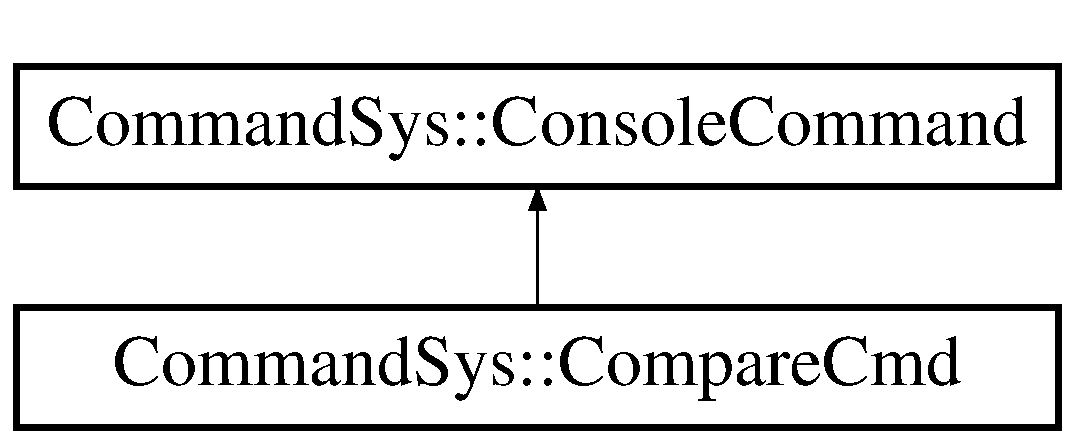
\includegraphics[height=2.000000cm]{class_command_sys_1_1_compare_cmd}
\end{center}
\end{figure}
\subsection*{Public 成员函数}
\begin{DoxyCompactItemize}
\item 
virtual void \hyperlink{class_command_sys_1_1_compare_cmd_a20c521a7bd9d1b92f6ef16416cf2784f}{Execute} (void)
\begin{DoxyCompactList}\small\item\em 执行命令 \end{DoxyCompactList}\item 
\hypertarget{class_command_sys_1_1_compare_cmd_a279dd1e78937c4f09f0b266adcfe9242}{virtual void {\bfseries Delete\-This} (void)}\label{class_command_sys_1_1_compare_cmd_a279dd1e78937c4f09f0b266adcfe9242}

\end{DoxyCompactItemize}
\subsection*{额外继承的成员函数}


\subsection{详细描述}


在文件 Compare\-Cmd.\-h 第 9 行定义.



\subsection{成员函数说明}
\hypertarget{class_command_sys_1_1_compare_cmd_a20c521a7bd9d1b92f6ef16416cf2784f}{\index{Command\-Sys\-::\-Compare\-Cmd@{Command\-Sys\-::\-Compare\-Cmd}!Execute@{Execute}}
\index{Execute@{Execute}!CommandSys::CompareCmd@{Command\-Sys\-::\-Compare\-Cmd}}
\subsubsection[{Execute}]{\setlength{\rightskip}{0pt plus 5cm}void Command\-Sys\-::\-Compare\-Cmd\-::\-Execute (
\begin{DoxyParamCaption}
\item[{void}]{}
\end{DoxyParamCaption}
)\hspace{0.3cm}{\ttfamily [virtual]}}}\label{class_command_sys_1_1_compare_cmd_a20c521a7bd9d1b92f6ef16416cf2784f}


执行命令 

\begin{DoxyRemark}{备注}
子类需重写该函数 
\end{DoxyRemark}


重载 \hyperlink{class_command_sys_1_1_console_command_a1d63e6780d3cfe83cc3452b0d797324c}{Command\-Sys\-::\-Console\-Command} .



在文件 Compare\-Cmd.\-cpp 第 17 行定义.



该类的文档由以下文件生成\-:\begin{DoxyCompactItemize}
\item 
Virtual\-Disk\-Console/Compare\-Cmd.\-h\item 
Virtual\-Disk\-Console/Compare\-Cmd.\-cpp\end{DoxyCompactItemize}

\hypertarget{class_command_sys_1_1_console_command}{\section{Command\-Sys\-:\-:Console\-Command类 参考}
\label{class_command_sys_1_1_console_command}\index{Command\-Sys\-::\-Console\-Command@{Command\-Sys\-::\-Console\-Command}}
}
类 Command\-Sys\-:\-:Console\-Command 继承关系图\-:\begin{figure}[H]
\begin{center}
\leavevmode
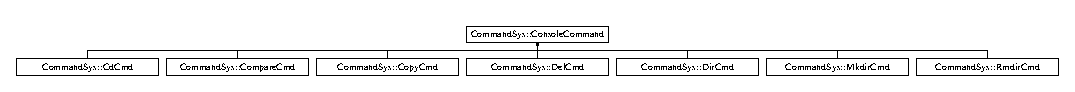
\includegraphics[height=0.788177cm]{class_command_sys_1_1_console_command}
\end{center}
\end{figure}
\subsection*{Public 成员函数}
\begin{DoxyCompactItemize}
\item 
void \hyperlink{class_command_sys_1_1_console_command_a630c500ae469cc33afa8f502b73adcb3}{Set\-Curr\-Path} (const Util\-::\-String \&curr\-\_\-path)
\begin{DoxyCompactList}\small\item\em 设置当前路径 \end{DoxyCompactList}\item 
void \hyperlink{class_command_sys_1_1_console_command_ad467ade07437eef25535a0fc8dc42a02}{Set\-Param\-Toks} (const \hyperlink{class_util_1_1_link_list_t}{Util\-::\-Link\-List\-T}$<$ \hyperlink{class_lexer_sys_1_1_token}{Lexer\-Sys\-::\-Token} $>$ \&params)
\begin{DoxyCompactList}\small\item\em 设置当前命令用户所输入的参数列表 \end{DoxyCompactList}\item 
void \hyperlink{class_command_sys_1_1_console_command_a28c05ba316393a029f5d6c708f4684b3}{Add\-Path} (const \hyperlink{class_lexer_sys_1_1_search_path}{Lexer\-Sys\-::\-Search\-Path} \&path)
\begin{DoxyCompactList}\small\item\em 将路径加入命令的路径列表 \end{DoxyCompactList}\item 
void \hyperlink{class_command_sys_1_1_console_command_a469dcbd51921716a279346b313082fec}{Set\-Paths} (const \hyperlink{class_util_1_1_link_list_t}{Util\-::\-Link\-List\-T}$<$ \hyperlink{class_lexer_sys_1_1_search_path}{Lexer\-Sys\-::\-Search\-Path} $>$ \&paths)
\begin{DoxyCompactList}\small\item\em 设置当前命令的路径列表 \end{DoxyCompactList}\item 
\hypertarget{class_command_sys_1_1_console_command_a775e8cf7b73354f05f44232b9310070e}{bool \hyperlink{class_command_sys_1_1_console_command_a775e8cf7b73354f05f44232b9310070e}{Is\-Path\-Length\-Out\-Of\-Limit} (void) const }\label{class_command_sys_1_1_console_command_a775e8cf7b73354f05f44232b9310070e}

\begin{DoxyCompactList}\small\item\em 判断用户输入的路径中是否有超过限定长度的路径 \end{DoxyCompactList}\item 
virtual void \hyperlink{class_command_sys_1_1_console_command_a1d63e6780d3cfe83cc3452b0d797324c}{Execute} (void)
\begin{DoxyCompactList}\small\item\em 执行命令 \end{DoxyCompactList}\item 
\hypertarget{class_command_sys_1_1_console_command_a380826ec9a19599d809966ae6ba3e70d}{Util\-::\-String \hyperlink{class_command_sys_1_1_console_command_a380826ec9a19599d809966ae6ba3e70d}{Get\-Result\-Output} (void)}\label{class_command_sys_1_1_console_command_a380826ec9a19599d809966ae6ba3e70d}

\begin{DoxyCompactList}\small\item\em 获得结果输出 \end{DoxyCompactList}\item 
\hypertarget{class_command_sys_1_1_console_command_a74acff251b68f7f1d7385a88ed4ad0b2}{Util\-::\-String \hyperlink{class_command_sys_1_1_console_command_a74acff251b68f7f1d7385a88ed4ad0b2}{Get\-Curr\-Path} (void)}\label{class_command_sys_1_1_console_command_a74acff251b68f7f1d7385a88ed4ad0b2}

\begin{DoxyCompactList}\small\item\em 获得当前路径字符串 \end{DoxyCompactList}\item 
\hypertarget{class_command_sys_1_1_console_command_a64da8f9370c53e11065885cae8c4140a}{virtual void {\bfseries Delete\-This} (void)}\label{class_command_sys_1_1_console_command_a64da8f9370c53e11065885cae8c4140a}

\end{DoxyCompactItemize}
\subsection*{Protected 成员函数}
\begin{DoxyCompactItemize}
\item 
\hyperlink{class_file_sys_1_1_node}{File\-Sys\-::\-Node} $\ast$ \hyperlink{class_command_sys_1_1_console_command_ad82b62c3e6220ad46c31d611f9e42e6b}{Search\-Curr\-Path\-Node} (void)
\begin{DoxyCompactList}\small\item\em 根据当前路径查找文件系统中对应的文件夹节点 \end{DoxyCompactList}\item 
\hyperlink{class_file_sys_1_1_node}{File\-Sys\-::\-Node} $\ast$ \hyperlink{class_command_sys_1_1_console_command_a2aab8c2ebe6250fb8fc7a41b1ad358c0}{Search\-Node\-By\-Path} (const \hyperlink{class_lexer_sys_1_1_search_path}{Lexer\-Sys\-::\-Search\-Path} \&path)
\begin{DoxyCompactList}\small\item\em 获得指定路径的文件系统节点 \end{DoxyCompactList}\end{DoxyCompactItemize}
\subsection*{Protected 属性}
\begin{DoxyCompactItemize}
\item 
\hypertarget{class_command_sys_1_1_console_command_a662c78fdb599ea9c15365fa716fe9106}{\hyperlink{class_lexer_sys_1_1_search_path}{Lexer\-Sys\-::\-Search\-Path} {\bfseries m\-\_\-curr\-\_\-path}}\label{class_command_sys_1_1_console_command_a662c78fdb599ea9c15365fa716fe9106}

\item 
\hypertarget{class_command_sys_1_1_console_command_a04f042e84f0979df89dfa4467dab9139}{\hyperlink{class_util_1_1_link_list_t}{Util\-::\-Link\-List\-T}$<$ \hyperlink{class_lexer_sys_1_1_token}{Lexer\-Sys\-::\-Token} $>$ \hyperlink{class_command_sys_1_1_console_command_a04f042e84f0979df89dfa4467dab9139}{m\-\_\-params}}\label{class_command_sys_1_1_console_command_a04f042e84f0979df89dfa4467dab9139}

\begin{DoxyCompactList}\small\item\em $>$当前路径 \end{DoxyCompactList}\item 
\hypertarget{class_command_sys_1_1_console_command_a947a59518b6441cb88f679deb13a5207}{\hyperlink{class_util_1_1_link_list_t}{Util\-::\-Link\-List\-T}\\*
$<$ \hyperlink{class_lexer_sys_1_1_search_path}{Lexer\-Sys\-::\-Search\-Path} $>$ \hyperlink{class_command_sys_1_1_console_command_a947a59518b6441cb88f679deb13a5207}{m\-\_\-paths}}\label{class_command_sys_1_1_console_command_a947a59518b6441cb88f679deb13a5207}

\begin{DoxyCompactList}\small\item\em $>$参数列表 \end{DoxyCompactList}\item 
\hypertarget{class_command_sys_1_1_console_command_af386498b8ae657e258f7c8a9c0569c98}{Util\-::\-String \hyperlink{class_command_sys_1_1_console_command_af386498b8ae657e258f7c8a9c0569c98}{m\-\_\-result\-\_\-output}}\label{class_command_sys_1_1_console_command_af386498b8ae657e258f7c8a9c0569c98}

\begin{DoxyCompactList}\small\item\em $>$路径列表 \end{DoxyCompactList}\end{DoxyCompactItemize}


\subsection{详细描述}


在文件 Console\-Command.\-h 第 11 行定义.



\subsection{成员函数说明}
\hypertarget{class_command_sys_1_1_console_command_a28c05ba316393a029f5d6c708f4684b3}{\index{Command\-Sys\-::\-Console\-Command@{Command\-Sys\-::\-Console\-Command}!Add\-Path@{Add\-Path}}
\index{Add\-Path@{Add\-Path}!CommandSys::ConsoleCommand@{Command\-Sys\-::\-Console\-Command}}
\subsubsection[{Add\-Path}]{\setlength{\rightskip}{0pt plus 5cm}void Command\-Sys\-::\-Console\-Command\-::\-Add\-Path (
\begin{DoxyParamCaption}
\item[{const {\bf Lexer\-Sys\-::\-Search\-Path} \&}]{path}
\end{DoxyParamCaption}
)}}\label{class_command_sys_1_1_console_command_a28c05ba316393a029f5d6c708f4684b3}


将路径加入命令的路径列表 


\begin{DoxyParams}{参数}
{\em path} & 要加入的路径 \\
\hline
\end{DoxyParams}


在文件 Console\-Command.\-cpp 第 30 行定义.

\hypertarget{class_command_sys_1_1_console_command_a1d63e6780d3cfe83cc3452b0d797324c}{\index{Command\-Sys\-::\-Console\-Command@{Command\-Sys\-::\-Console\-Command}!Execute@{Execute}}
\index{Execute@{Execute}!CommandSys::ConsoleCommand@{Command\-Sys\-::\-Console\-Command}}
\subsubsection[{Execute}]{\setlength{\rightskip}{0pt plus 5cm}virtual void Command\-Sys\-::\-Console\-Command\-::\-Execute (
\begin{DoxyParamCaption}
\item[{void}]{}
\end{DoxyParamCaption}
)\hspace{0.3cm}{\ttfamily [inline]}, {\ttfamily [virtual]}}}\label{class_command_sys_1_1_console_command_a1d63e6780d3cfe83cc3452b0d797324c}


执行命令 

\begin{DoxyRemark}{备注}
子类需重写该函数 
\end{DoxyRemark}


被 \hyperlink{class_command_sys_1_1_cd_cmd_af355386817b6cad86d370d65267d5d88}{Command\-Sys\-::\-Cd\-Cmd}, \hyperlink{class_command_sys_1_1_compare_cmd_a20c521a7bd9d1b92f6ef16416cf2784f}{Command\-Sys\-::\-Compare\-Cmd}, \hyperlink{class_command_sys_1_1_copy_cmd_a4b094e7c2d79541444b0ee561b2b7464}{Command\-Sys\-::\-Copy\-Cmd}, \hyperlink{class_command_sys_1_1_del_cmd_a8b843ea865167bd3de7eef3f1902a463}{Command\-Sys\-::\-Del\-Cmd}, \hyperlink{class_command_sys_1_1_dir_cmd_ac19a660aea728dae9ab2161c63c945e9}{Command\-Sys\-::\-Dir\-Cmd}, \hyperlink{class_command_sys_1_1_mkdir_cmd_a6a4c23d4e458c2ab12ca9da07625c1e1}{Command\-Sys\-::\-Mkdir\-Cmd} , 以及 \hyperlink{class_command_sys_1_1_rmdir_cmd_a66d3b433eecba42b9f00f7fc3f09f623}{Command\-Sys\-::\-Rmdir\-Cmd} 重载.



在文件 Console\-Command.\-h 第 50 行定义.

\hypertarget{class_command_sys_1_1_console_command_ad82b62c3e6220ad46c31d611f9e42e6b}{\index{Command\-Sys\-::\-Console\-Command@{Command\-Sys\-::\-Console\-Command}!Search\-Curr\-Path\-Node@{Search\-Curr\-Path\-Node}}
\index{Search\-Curr\-Path\-Node@{Search\-Curr\-Path\-Node}!CommandSys::ConsoleCommand@{Command\-Sys\-::\-Console\-Command}}
\subsubsection[{Search\-Curr\-Path\-Node}]{\setlength{\rightskip}{0pt plus 5cm}{\bf File\-Sys\-::\-Node} $\ast$ Command\-Sys\-::\-Console\-Command\-::\-Search\-Curr\-Path\-Node (
\begin{DoxyParamCaption}
\item[{void}]{}
\end{DoxyParamCaption}
)\hspace{0.3cm}{\ttfamily [protected]}}}\label{class_command_sys_1_1_console_command_ad82b62c3e6220ad46c31d611f9e42e6b}


根据当前路径查找文件系统中对应的文件夹节点 

\begin{DoxyReturn}{返回}
指向找到的当前路径节点指针 
\end{DoxyReturn}


在文件 Console\-Command.\-cpp 第 69 行定义.

\hypertarget{class_command_sys_1_1_console_command_a2aab8c2ebe6250fb8fc7a41b1ad358c0}{\index{Command\-Sys\-::\-Console\-Command@{Command\-Sys\-::\-Console\-Command}!Search\-Node\-By\-Path@{Search\-Node\-By\-Path}}
\index{Search\-Node\-By\-Path@{Search\-Node\-By\-Path}!CommandSys::ConsoleCommand@{Command\-Sys\-::\-Console\-Command}}
\subsubsection[{Search\-Node\-By\-Path}]{\setlength{\rightskip}{0pt plus 5cm}{\bf File\-Sys\-::\-Node} $\ast$ Command\-Sys\-::\-Console\-Command\-::\-Search\-Node\-By\-Path (
\begin{DoxyParamCaption}
\item[{const {\bf Lexer\-Sys\-::\-Search\-Path} \&}]{path}
\end{DoxyParamCaption}
)\hspace{0.3cm}{\ttfamily [protected]}}}\label{class_command_sys_1_1_console_command_a2aab8c2ebe6250fb8fc7a41b1ad358c0}


获得指定路径的文件系统节点 

\begin{DoxyReturn}{返回}
指向找到路径节点的指针 
\end{DoxyReturn}

\begin{DoxyRetVals}{返回值}
{\em N\-U\-L\-L} & 查找失败,文件系统中没有该路径所表示的节点 \\
\hline
{\em not} & N\-U\-L\-L 查找成功 \\
\hline
\end{DoxyRetVals}


在文件 Console\-Command.\-cpp 第 50 行定义.

\hypertarget{class_command_sys_1_1_console_command_a630c500ae469cc33afa8f502b73adcb3}{\index{Command\-Sys\-::\-Console\-Command@{Command\-Sys\-::\-Console\-Command}!Set\-Curr\-Path@{Set\-Curr\-Path}}
\index{Set\-Curr\-Path@{Set\-Curr\-Path}!CommandSys::ConsoleCommand@{Command\-Sys\-::\-Console\-Command}}
\subsubsection[{Set\-Curr\-Path}]{\setlength{\rightskip}{0pt plus 5cm}void Command\-Sys\-::\-Console\-Command\-::\-Set\-Curr\-Path (
\begin{DoxyParamCaption}
\item[{const Util\-::\-String \&}]{curr\-\_\-path}
\end{DoxyParamCaption}
)}}\label{class_command_sys_1_1_console_command_a630c500ae469cc33afa8f502b73adcb3}


设置当前路径 


\begin{DoxyParams}{参数}
{\em curr\-\_\-path} & 当前路径字符串 \\
\hline
\end{DoxyParams}


在文件 Console\-Command.\-cpp 第 19 行定义.

\hypertarget{class_command_sys_1_1_console_command_ad467ade07437eef25535a0fc8dc42a02}{\index{Command\-Sys\-::\-Console\-Command@{Command\-Sys\-::\-Console\-Command}!Set\-Param\-Toks@{Set\-Param\-Toks}}
\index{Set\-Param\-Toks@{Set\-Param\-Toks}!CommandSys::ConsoleCommand@{Command\-Sys\-::\-Console\-Command}}
\subsubsection[{Set\-Param\-Toks}]{\setlength{\rightskip}{0pt plus 5cm}void Command\-Sys\-::\-Console\-Command\-::\-Set\-Param\-Toks (
\begin{DoxyParamCaption}
\item[{const {\bf Util\-::\-Link\-List\-T}$<$ {\bf Lexer\-Sys\-::\-Token} $>$ \&}]{params}
\end{DoxyParamCaption}
)}}\label{class_command_sys_1_1_console_command_ad467ade07437eef25535a0fc8dc42a02}


设置当前命令用户所输入的参数列表 


\begin{DoxyParams}{参数}
{\em params} & 用户输入的参数列表 \\
\hline
\end{DoxyParams}


在文件 Console\-Command.\-cpp 第 25 行定义.

\hypertarget{class_command_sys_1_1_console_command_a469dcbd51921716a279346b313082fec}{\index{Command\-Sys\-::\-Console\-Command@{Command\-Sys\-::\-Console\-Command}!Set\-Paths@{Set\-Paths}}
\index{Set\-Paths@{Set\-Paths}!CommandSys::ConsoleCommand@{Command\-Sys\-::\-Console\-Command}}
\subsubsection[{Set\-Paths}]{\setlength{\rightskip}{0pt plus 5cm}void Command\-Sys\-::\-Console\-Command\-::\-Set\-Paths (
\begin{DoxyParamCaption}
\item[{const {\bf Util\-::\-Link\-List\-T}$<$ {\bf Lexer\-Sys\-::\-Search\-Path} $>$ \&}]{paths}
\end{DoxyParamCaption}
)}}\label{class_command_sys_1_1_console_command_a469dcbd51921716a279346b313082fec}


设置当前命令的路径列表 


\begin{DoxyParams}{参数}
{\em paths} & 要设置的路径列表 \\
\hline
\end{DoxyParams}


在文件 Console\-Command.\-cpp 第 35 行定义.



该类的文档由以下文件生成\-:\begin{DoxyCompactItemize}
\item 
Virtual\-Disk\-Console/Console\-Command.\-h\item 
Virtual\-Disk\-Console/Console\-Command.\-cpp\end{DoxyCompactItemize}

\hypertarget{class_command_sys_1_1_console_command_factory}{\section{Command\-Sys\-:\-:Console\-Command\-Factory类 参考}
\label{class_command_sys_1_1_console_command_factory}\index{Command\-Sys\-::\-Console\-Command\-Factory@{Command\-Sys\-::\-Console\-Command\-Factory}}
}
类 Command\-Sys\-:\-:Console\-Command\-Factory 继承关系图\-:\begin{figure}[H]
\begin{center}
\leavevmode
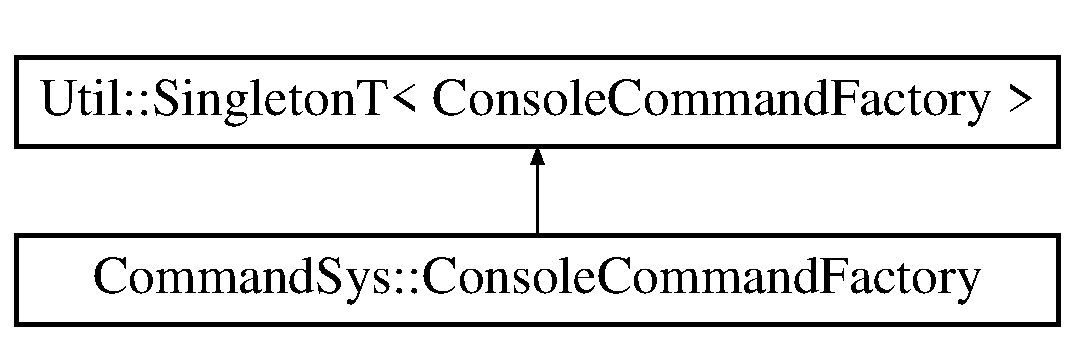
\includegraphics[height=2.000000cm]{class_command_sys_1_1_console_command_factory}
\end{center}
\end{figure}
\subsection*{Public 成员函数}
\begin{DoxyCompactItemize}
\item 
\hyperlink{class_command_sys_1_1_console_command}{Console\-Command} $\ast$ \hyperlink{class_command_sys_1_1_console_command_factory_a8f84a2b079f27ae225c0923f9b268d5c}{Create\-Command} (const Util\-::\-String \&curr\-\_\-path, const Util\-::\-String \&cmd)
\begin{DoxyCompactList}\small\item\em 根据用户的命令输入字符串创建命令对象 \end{DoxyCompactList}\end{DoxyCompactItemize}
\subsection*{额外继承的成员函数}


\subsection{详细描述}


在文件 Console\-Command\-Factory.\-h 第 9 行定义.



\subsection{成员函数说明}
\hypertarget{class_command_sys_1_1_console_command_factory_a8f84a2b079f27ae225c0923f9b268d5c}{\index{Command\-Sys\-::\-Console\-Command\-Factory@{Command\-Sys\-::\-Console\-Command\-Factory}!Create\-Command@{Create\-Command}}
\index{Create\-Command@{Create\-Command}!CommandSys::ConsoleCommandFactory@{Command\-Sys\-::\-Console\-Command\-Factory}}
\subsubsection[{Create\-Command}]{\setlength{\rightskip}{0pt plus 5cm}{\bf Console\-Command} $\ast$ Command\-Sys\-::\-Console\-Command\-Factory\-::\-Create\-Command (
\begin{DoxyParamCaption}
\item[{const Util\-::\-String \&}]{curr\-\_\-path, }
\item[{const Util\-::\-String \&}]{cmd}
\end{DoxyParamCaption}
)}}\label{class_command_sys_1_1_console_command_factory_a8f84a2b079f27ae225c0923f9b268d5c}


根据用户的命令输入字符串创建命令对象 


\begin{DoxyParams}{参数}
{\em curr\-\_\-path} & 用户的当前路径 \\
\hline
{\em cmd} & 用户输入的命令字符串 \\
\hline
\end{DoxyParams}
\begin{DoxyReturn}{返回}
命令对象指针 
\end{DoxyReturn}


在文件 Console\-Command\-Factory.\-cpp 第 25 行定义.



该类的文档由以下文件生成\-:\begin{DoxyCompactItemize}
\item 
Virtual\-Disk\-Console/Console\-Command\-Factory.\-h\item 
Virtual\-Disk\-Console/Console\-Command\-Factory.\-cpp\end{DoxyCompactItemize}

\hypertarget{class_command_sys_1_1_copy_cmd}{\section{Command\-Sys\-:\-:Copy\-Cmd类 参考}
\label{class_command_sys_1_1_copy_cmd}\index{Command\-Sys\-::\-Copy\-Cmd@{Command\-Sys\-::\-Copy\-Cmd}}
}
类 Command\-Sys\-:\-:Copy\-Cmd 继承关系图\-:\begin{figure}[H]
\begin{center}
\leavevmode
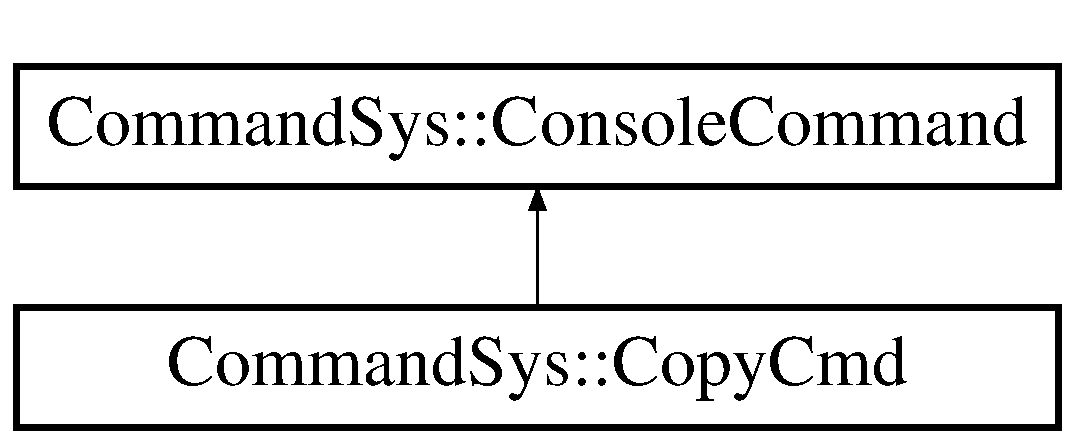
\includegraphics[height=2.000000cm]{class_command_sys_1_1_copy_cmd}
\end{center}
\end{figure}
\subsection*{Public 成员函数}
\begin{DoxyCompactItemize}
\item 
virtual void \hyperlink{class_command_sys_1_1_copy_cmd_a4b094e7c2d79541444b0ee561b2b7464}{Execute} (void)
\begin{DoxyCompactList}\small\item\em 执行命令 \end{DoxyCompactList}\item 
\hypertarget{class_command_sys_1_1_copy_cmd_a34f98b273c2159aeea376c59d99a6809}{virtual void {\bfseries Delete\-This} (void)}\label{class_command_sys_1_1_copy_cmd_a34f98b273c2159aeea376c59d99a6809}

\end{DoxyCompactItemize}
\subsection*{额外继承的成员函数}


\subsection{详细描述}


在文件 Copy\-Cmd.\-h 第 9 行定义.



\subsection{成员函数说明}
\hypertarget{class_command_sys_1_1_copy_cmd_a4b094e7c2d79541444b0ee561b2b7464}{\index{Command\-Sys\-::\-Copy\-Cmd@{Command\-Sys\-::\-Copy\-Cmd}!Execute@{Execute}}
\index{Execute@{Execute}!CommandSys::CopyCmd@{Command\-Sys\-::\-Copy\-Cmd}}
\subsubsection[{Execute}]{\setlength{\rightskip}{0pt plus 5cm}void Command\-Sys\-::\-Copy\-Cmd\-::\-Execute (
\begin{DoxyParamCaption}
\item[{void}]{}
\end{DoxyParamCaption}
)\hspace{0.3cm}{\ttfamily [virtual]}}}\label{class_command_sys_1_1_copy_cmd_a4b094e7c2d79541444b0ee561b2b7464}


执行命令 

\begin{DoxyRemark}{备注}
子类需重写该函数 
\end{DoxyRemark}


重载 \hyperlink{class_command_sys_1_1_console_command_a1d63e6780d3cfe83cc3452b0d797324c}{Command\-Sys\-::\-Console\-Command} .



在文件 Copy\-Cmd.\-cpp 第 18 行定义.



该类的文档由以下文件生成\-:\begin{DoxyCompactItemize}
\item 
Virtual\-Disk\-Console/Copy\-Cmd.\-h\item 
Virtual\-Disk\-Console/Copy\-Cmd.\-cpp\end{DoxyCompactItemize}

\hypertarget{class_file_sys_1_1_create_dir_visitor}{\section{File\-Sys\-:\-:Create\-Dir\-Visitor类 参考}
\label{class_file_sys_1_1_create_dir_visitor}\index{File\-Sys\-::\-Create\-Dir\-Visitor@{File\-Sys\-::\-Create\-Dir\-Visitor}}
}
类 File\-Sys\-:\-:Create\-Dir\-Visitor 继承关系图\-:\begin{figure}[H]
\begin{center}
\leavevmode
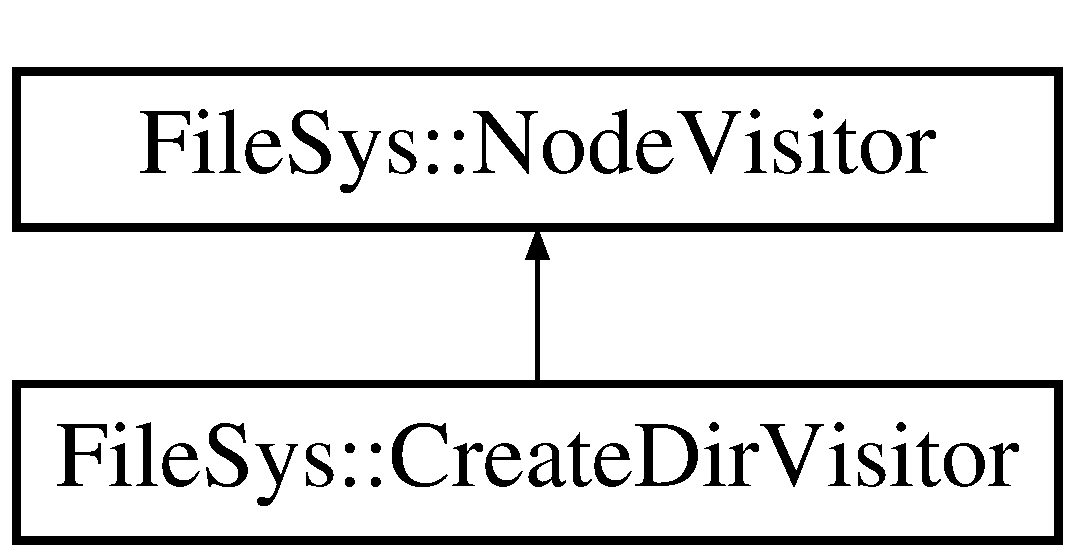
\includegraphics[height=2.000000cm]{class_file_sys_1_1_create_dir_visitor}
\end{center}
\end{figure}
\subsection*{Public 成员函数}
\begin{DoxyCompactItemize}
\item 
virtual void \hyperlink{class_file_sys_1_1_create_dir_visitor_a02c79d46c769edbbcff38a59a97811ab}{Visit} (\hyperlink{class_file_sys_1_1_node}{Node} $\ast$node)
\begin{DoxyCompactList}\small\item\em 访问节点 \end{DoxyCompactList}\end{DoxyCompactItemize}
\subsection*{额外继承的成员函数}


\subsection{详细描述}


在文件 Create\-Dir\-Visitor.\-h 第 9 行定义.



\subsection{成员函数说明}
\hypertarget{class_file_sys_1_1_create_dir_visitor_a02c79d46c769edbbcff38a59a97811ab}{\index{File\-Sys\-::\-Create\-Dir\-Visitor@{File\-Sys\-::\-Create\-Dir\-Visitor}!Visit@{Visit}}
\index{Visit@{Visit}!FileSys::CreateDirVisitor@{File\-Sys\-::\-Create\-Dir\-Visitor}}
\subsubsection[{Visit}]{\setlength{\rightskip}{0pt plus 5cm}void File\-Sys\-::\-Create\-Dir\-Visitor\-::\-Visit (
\begin{DoxyParamCaption}
\item[{{\bf Node} $\ast$}]{node}
\end{DoxyParamCaption}
)\hspace{0.3cm}{\ttfamily [virtual]}}}\label{class_file_sys_1_1_create_dir_visitor_a02c79d46c769edbbcff38a59a97811ab}


访问节点 


\begin{DoxyParams}{参数}
{\em node} & 待访问节点 \\
\hline
\end{DoxyParams}


重载 \hyperlink{class_file_sys_1_1_node_visitor_a3398560bc10e71a0b8fcaac57e5b58e2}{File\-Sys\-::\-Node\-Visitor} .



在文件 Create\-Dir\-Visitor.\-cpp 第 16 行定义.



该类的文档由以下文件生成\-:\begin{DoxyCompactItemize}
\item 
Virtual\-Disk\-Console/Create\-Dir\-Visitor.\-h\item 
Virtual\-Disk\-Console/Create\-Dir\-Visitor.\-cpp\end{DoxyCompactItemize}

\hypertarget{class_command_sys_1_1_del_cmd}{\section{Command\-Sys\-:\-:Del\-Cmd类 参考}
\label{class_command_sys_1_1_del_cmd}\index{Command\-Sys\-::\-Del\-Cmd@{Command\-Sys\-::\-Del\-Cmd}}
}
类 Command\-Sys\-:\-:Del\-Cmd 继承关系图\-:\begin{figure}[H]
\begin{center}
\leavevmode
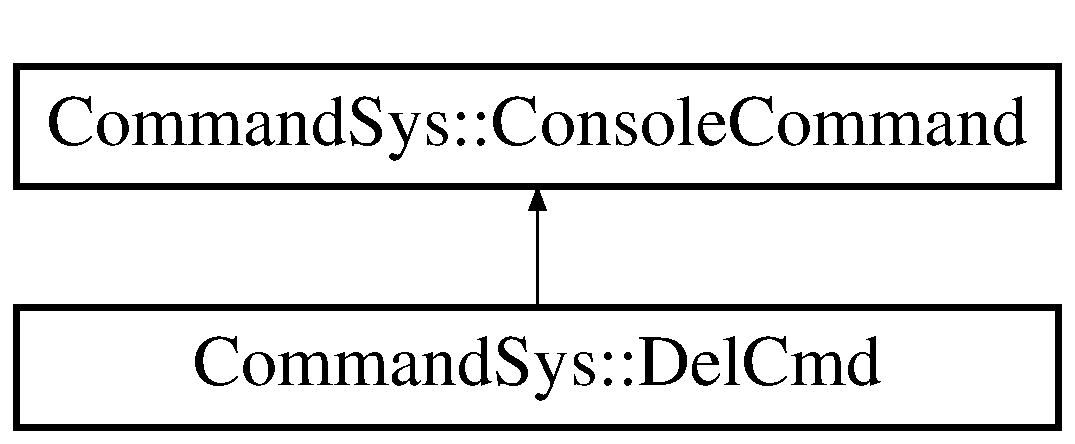
\includegraphics[height=2.000000cm]{class_command_sys_1_1_del_cmd}
\end{center}
\end{figure}
\subsection*{Public 成员函数}
\begin{DoxyCompactItemize}
\item 
virtual void \hyperlink{class_command_sys_1_1_del_cmd_a8b843ea865167bd3de7eef3f1902a463}{Execute} (void)
\begin{DoxyCompactList}\small\item\em 执行命令 \end{DoxyCompactList}\item 
\hypertarget{class_command_sys_1_1_del_cmd_a87a1da99fc98cd7c7439ee0d73fd5a5a}{virtual void {\bfseries Delete\-This} (void)}\label{class_command_sys_1_1_del_cmd_a87a1da99fc98cd7c7439ee0d73fd5a5a}

\end{DoxyCompactItemize}
\subsection*{额外继承的成员函数}


\subsection{详细描述}


在文件 Del\-Cmd.\-h 第 9 行定义.



\subsection{成员函数说明}
\hypertarget{class_command_sys_1_1_del_cmd_a8b843ea865167bd3de7eef3f1902a463}{\index{Command\-Sys\-::\-Del\-Cmd@{Command\-Sys\-::\-Del\-Cmd}!Execute@{Execute}}
\index{Execute@{Execute}!CommandSys::DelCmd@{Command\-Sys\-::\-Del\-Cmd}}
\subsubsection[{Execute}]{\setlength{\rightskip}{0pt plus 5cm}void Command\-Sys\-::\-Del\-Cmd\-::\-Execute (
\begin{DoxyParamCaption}
\item[{void}]{}
\end{DoxyParamCaption}
)\hspace{0.3cm}{\ttfamily [virtual]}}}\label{class_command_sys_1_1_del_cmd_a8b843ea865167bd3de7eef3f1902a463}


执行命令 

\begin{DoxyRemark}{备注}
子类需重写该函数 
\end{DoxyRemark}


重载 \hyperlink{class_command_sys_1_1_console_command_a1d63e6780d3cfe83cc3452b0d797324c}{Command\-Sys\-::\-Console\-Command} .



在文件 Del\-Cmd.\-cpp 第 15 行定义.



该类的文档由以下文件生成\-:\begin{DoxyCompactItemize}
\item 
Virtual\-Disk\-Console/Del\-Cmd.\-h\item 
Virtual\-Disk\-Console/Del\-Cmd.\-cpp\end{DoxyCompactItemize}

\hypertarget{class_command_sys_1_1_dir_cmd}{\section{Command\-Sys\-:\-:Dir\-Cmd类 参考}
\label{class_command_sys_1_1_dir_cmd}\index{Command\-Sys\-::\-Dir\-Cmd@{Command\-Sys\-::\-Dir\-Cmd}}
}
类 Command\-Sys\-:\-:Dir\-Cmd 继承关系图\-:\begin{figure}[H]
\begin{center}
\leavevmode
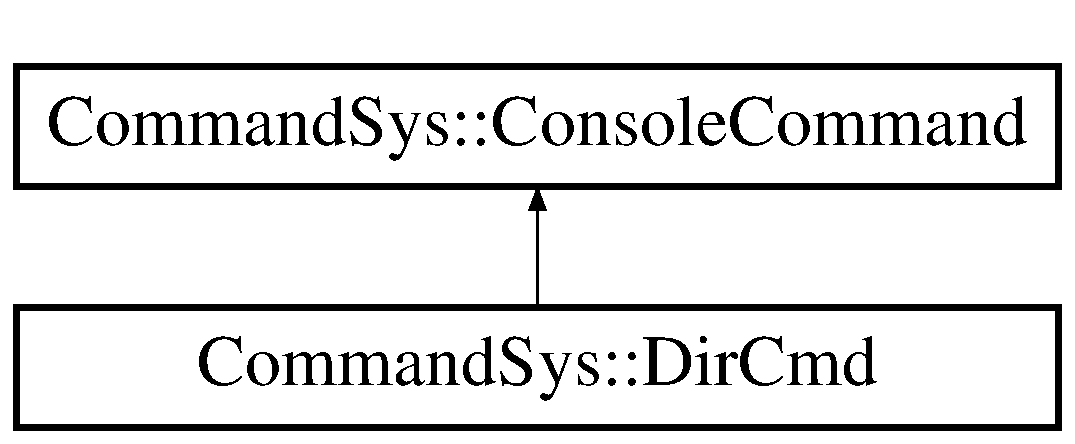
\includegraphics[height=2.000000cm]{class_command_sys_1_1_dir_cmd}
\end{center}
\end{figure}
\subsection*{Public 成员函数}
\begin{DoxyCompactItemize}
\item 
virtual void \hyperlink{class_command_sys_1_1_dir_cmd_ac19a660aea728dae9ab2161c63c945e9}{Execute} (void)
\begin{DoxyCompactList}\small\item\em 执行命令 \end{DoxyCompactList}\item 
\hypertarget{class_command_sys_1_1_dir_cmd_adb386912dae8856edf4db5311b5117b6}{virtual void {\bfseries Delete\-This} (void)}\label{class_command_sys_1_1_dir_cmd_adb386912dae8856edf4db5311b5117b6}

\end{DoxyCompactItemize}
\subsection*{额外继承的成员函数}


\subsection{详细描述}


在文件 Dir\-Cmd.\-h 第 9 行定义.



\subsection{成员函数说明}
\hypertarget{class_command_sys_1_1_dir_cmd_ac19a660aea728dae9ab2161c63c945e9}{\index{Command\-Sys\-::\-Dir\-Cmd@{Command\-Sys\-::\-Dir\-Cmd}!Execute@{Execute}}
\index{Execute@{Execute}!CommandSys::DirCmd@{Command\-Sys\-::\-Dir\-Cmd}}
\subsubsection[{Execute}]{\setlength{\rightskip}{0pt plus 5cm}void Command\-Sys\-::\-Dir\-Cmd\-::\-Execute (
\begin{DoxyParamCaption}
\item[{void}]{}
\end{DoxyParamCaption}
)\hspace{0.3cm}{\ttfamily [virtual]}}}\label{class_command_sys_1_1_dir_cmd_ac19a660aea728dae9ab2161c63c945e9}


执行命令 

\begin{DoxyRemark}{备注}
子类需重写该函数 
\end{DoxyRemark}


重载 \hyperlink{class_command_sys_1_1_console_command_a1d63e6780d3cfe83cc3452b0d797324c}{Command\-Sys\-::\-Console\-Command} .



在文件 Dir\-Cmd.\-cpp 第 15 行定义.



该类的文档由以下文件生成\-:\begin{DoxyCompactItemize}
\item 
Virtual\-Disk\-Console/Dir\-Cmd.\-h\item 
Virtual\-Disk\-Console/Dir\-Cmd.\-cpp\end{DoxyCompactItemize}

\hypertarget{class_file_sys_1_1_file_node}{\section{File\-Sys\-:\-:File\-Node类 参考}
\label{class_file_sys_1_1_file_node}\index{File\-Sys\-::\-File\-Node@{File\-Sys\-::\-File\-Node}}
}
类 File\-Sys\-:\-:File\-Node 继承关系图\-:\begin{figure}[H]
\begin{center}
\leavevmode
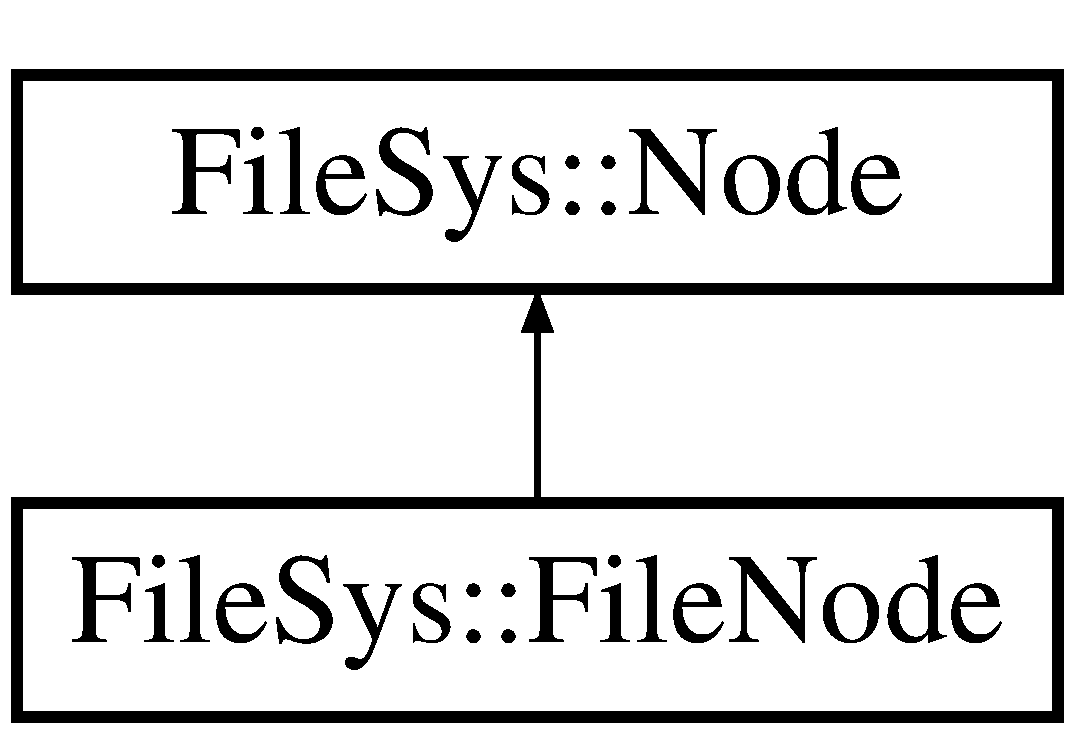
\includegraphics[height=2.000000cm]{class_file_sys_1_1_file_node}
\end{center}
\end{figure}
\subsection*{Public 成员函数}
\begin{DoxyCompactItemize}
\item 
\hypertarget{class_file_sys_1_1_file_node_a8a9c01da1c043554743877aff68ddad9}{virtual bool \hyperlink{class_file_sys_1_1_file_node_a8a9c01da1c043554743877aff68ddad9}{Is\-File} (void) const }\label{class_file_sys_1_1_file_node_a8a9c01da1c043554743877aff68ddad9}

\begin{DoxyCompactList}\small\item\em 判断该节点是否为文件 \end{DoxyCompactList}\item 
virtual bool \hyperlink{class_file_sys_1_1_file_node_a0bf53af4d6c34922bc1c667415b65d5c}{Is\-Binary\-File} (void) const 
\begin{DoxyCompactList}\small\item\em 根据文件名来判断当前文件是否为二进制文件 \end{DoxyCompactList}\item 
virtual int \hyperlink{class_file_sys_1_1_file_node_a4284926acb04ef0ab0db8b73d2f1fba1}{Copy} (const void $\ast$data, const D\-W\-O\-R\-D size)
\begin{DoxyCompactList}\small\item\em 将传入的数据拷贝给该文件 \end{DoxyCompactList}\item 
virtual int \hyperlink{class_file_sys_1_1_file_node_a63de509985ada5a7cedfc46c1e4e1277}{Read} (const D\-W\-O\-R\-D offset, const D\-W\-O\-R\-D size, void $\ast$data)
\begin{DoxyCompactList}\small\item\em 读取虚拟磁盘中文件数据 \end{DoxyCompactList}\item 
\hypertarget{class_file_sys_1_1_file_node_ab19cd336df69c6d8cdededa53486d63a}{virtual void \hyperlink{class_file_sys_1_1_file_node_ab19cd336df69c6d8cdededa53486d63a}{Clear\-Data} (void)}\label{class_file_sys_1_1_file_node_ab19cd336df69c6d8cdededa53486d63a}

\begin{DoxyCompactList}\small\item\em 清空节点中附带的数据 \end{DoxyCompactList}\item 
virtual D\-W\-O\-R\-D \hyperlink{class_file_sys_1_1_file_node_ac66c3549ac94e6ca8e5adde3970f6421}{Size} (void) const 
\begin{DoxyCompactList}\small\item\em 此文件节点数据的大小 \end{DoxyCompactList}\item 
virtual D\-W\-O\-R\-D \hyperlink{class_file_sys_1_1_file_node_acafc6eec61aafcf3e1899c9716ee3629}{Calc\-Total\-Size} (void)
\begin{DoxyCompactList}\small\item\em 递归计算该节点子树附带数据的总大小 \end{DoxyCompactList}\item 
virtual bool \hyperlink{class_file_sys_1_1_file_node_afd998a6e6747f426c856ccdedd21eeb6}{Compare} (const void $\ast$data, const D\-W\-O\-R\-D size, \hyperlink{class_util_1_1_vector_t}{Util\-::\-Vector\-T}$<$ char $>$ \&diff1, \hyperlink{class_util_1_1_vector_t}{Util\-::\-Vector\-T}$<$ char $>$ \&diff2) const 
\begin{DoxyCompactList}\small\item\em 比较指定缓冲区与当前文件的异同 \end{DoxyCompactList}\item 
virtual bool \hyperlink{class_file_sys_1_1_file_node_aa14e75686fe236425f4580763bd75222}{Compare} (const H\-A\-N\-D\-L\-E file, \hyperlink{class_util_1_1_vector_t}{Util\-::\-Vector\-T}$<$ char $>$ \&diff1, \hyperlink{class_util_1_1_vector_t}{Util\-::\-Vector\-T}$<$ char $>$ \&diff2) const 
\begin{DoxyCompactList}\small\item\em 比较指定缓冲区与当前文件的异同 \end{DoxyCompactList}\item 
\hypertarget{class_file_sys_1_1_file_node_aec88555b8c435e277a88d65814fb16eb}{virtual void \hyperlink{class_file_sys_1_1_file_node_aec88555b8c435e277a88d65814fb16eb}{Delete\-This} (void)}\label{class_file_sys_1_1_file_node_aec88555b8c435e277a88d65814fb16eb}

\begin{DoxyCompactList}\small\item\em 删除自身 \end{DoxyCompactList}\end{DoxyCompactItemize}
\subsection*{额外继承的成员函数}


\subsection{详细描述}


在文件 File\-Node.\-h 第 9 行定义.



\subsection{成员函数说明}
\hypertarget{class_file_sys_1_1_file_node_acafc6eec61aafcf3e1899c9716ee3629}{\index{File\-Sys\-::\-File\-Node@{File\-Sys\-::\-File\-Node}!Calc\-Total\-Size@{Calc\-Total\-Size}}
\index{Calc\-Total\-Size@{Calc\-Total\-Size}!FileSys::FileNode@{File\-Sys\-::\-File\-Node}}
\subsubsection[{Calc\-Total\-Size}]{\setlength{\rightskip}{0pt plus 5cm}virtual D\-W\-O\-R\-D File\-Sys\-::\-File\-Node\-::\-Calc\-Total\-Size (
\begin{DoxyParamCaption}
\item[{void}]{}
\end{DoxyParamCaption}
)\hspace{0.3cm}{\ttfamily [inline]}, {\ttfamily [virtual]}}}\label{class_file_sys_1_1_file_node_acafc6eec61aafcf3e1899c9716ee3629}


递归计算该节点子树附带数据的总大小 

\begin{DoxyReturn}{返回}
返回递归计算的子树附带数据大小 
\end{DoxyReturn}


重载 \hyperlink{class_file_sys_1_1_node_a6f73b0fcebfed60297a7472a954be9eb}{File\-Sys\-::\-Node} .



在文件 File\-Node.\-h 第 56 行定义.

\hypertarget{class_file_sys_1_1_file_node_afd998a6e6747f426c856ccdedd21eeb6}{\index{File\-Sys\-::\-File\-Node@{File\-Sys\-::\-File\-Node}!Compare@{Compare}}
\index{Compare@{Compare}!FileSys::FileNode@{File\-Sys\-::\-File\-Node}}
\subsubsection[{Compare}]{\setlength{\rightskip}{0pt plus 5cm}bool File\-Sys\-::\-File\-Node\-::\-Compare (
\begin{DoxyParamCaption}
\item[{const void $\ast$}]{data, }
\item[{const D\-W\-O\-R\-D}]{size, }
\item[{{\bf Util\-::\-Vector\-T}$<$ char $>$ \&}]{diff1, }
\item[{{\bf Util\-::\-Vector\-T}$<$ char $>$ \&}]{diff2}
\end{DoxyParamCaption}
) const\hspace{0.3cm}{\ttfamily [virtual]}}}\label{class_file_sys_1_1_file_node_afd998a6e6747f426c856ccdedd21eeb6}


比较指定缓冲区与当前文件的异同 


\begin{DoxyParams}{参数}
{\em data} & 待比较的缓冲区 \\
\hline
{\em size} & 缓冲区中数据的大小 \\
\hline
{\em diff1} & 返回的本文件从第一个不同字节起始处往后的16个字节数组 \\
\hline
{\em diff2} & 返回的磁盘文件从第一个不同字节起始处往后的16个字节数组 \\
\hline
\end{DoxyParams}
\begin{DoxyReturn}{返回}
返回比较是否相同 
\end{DoxyReturn}

\begin{DoxyRetVals}{返回值}
{\em true} & 比较结果相同 \\
\hline
{\em false} & 比较结果不同 \\
\hline
\end{DoxyRetVals}
\begin{DoxyRemark}{备注}
若data为\-N\-U\-L\-L或size为0的情况下也会返回false 
\end{DoxyRemark}


重载 \hyperlink{class_file_sys_1_1_node_ada9acb89cd979b2e37d169d67e9ba816}{File\-Sys\-::\-Node} .



在文件 File\-Node.\-cpp 第 25 行定义.

\hypertarget{class_file_sys_1_1_file_node_aa14e75686fe236425f4580763bd75222}{\index{File\-Sys\-::\-File\-Node@{File\-Sys\-::\-File\-Node}!Compare@{Compare}}
\index{Compare@{Compare}!FileSys::FileNode@{File\-Sys\-::\-File\-Node}}
\subsubsection[{Compare}]{\setlength{\rightskip}{0pt plus 5cm}bool File\-Sys\-::\-File\-Node\-::\-Compare (
\begin{DoxyParamCaption}
\item[{const H\-A\-N\-D\-L\-E}]{file, }
\item[{{\bf Util\-::\-Vector\-T}$<$ char $>$ \&}]{diff1, }
\item[{{\bf Util\-::\-Vector\-T}$<$ char $>$ \&}]{diff2}
\end{DoxyParamCaption}
) const\hspace{0.3cm}{\ttfamily [virtual]}}}\label{class_file_sys_1_1_file_node_aa14e75686fe236425f4580763bd75222}


比较指定缓冲区与当前文件的异同 


\begin{DoxyParams}{参数}
{\em file} & 待比较的磁盘文件句柄 \\
\hline
{\em diff1} & 返回的本文件从第一个不同字节起始处往后的16个字节数组 \\
\hline
{\em diff2} & 返回的磁盘文件从第一个不同字节起始处往后的16个字节数组 \\
\hline
\end{DoxyParams}
\begin{DoxyReturn}{返回}
返回比较是否相同 
\end{DoxyReturn}

\begin{DoxyRetVals}{返回值}
{\em true} & 比较结果相同 \\
\hline
{\em false} & 比较结果不同 \\
\hline
\end{DoxyRetVals}
\begin{DoxyRemark}{备注}
若data为\-N\-U\-L\-L或size为0的情况下也会返回false 
\end{DoxyRemark}


重载 \hyperlink{class_file_sys_1_1_node_a61fe784ffa56a134715baa35a5a7e239}{File\-Sys\-::\-Node} .



在文件 File\-Node.\-cpp 第 72 行定义.

\hypertarget{class_file_sys_1_1_file_node_a4284926acb04ef0ab0db8b73d2f1fba1}{\index{File\-Sys\-::\-File\-Node@{File\-Sys\-::\-File\-Node}!Copy@{Copy}}
\index{Copy@{Copy}!FileSys::FileNode@{File\-Sys\-::\-File\-Node}}
\subsubsection[{Copy}]{\setlength{\rightskip}{0pt plus 5cm}int File\-Sys\-::\-File\-Node\-::\-Copy (
\begin{DoxyParamCaption}
\item[{const void $\ast$}]{data, }
\item[{const D\-W\-O\-R\-D}]{size}
\end{DoxyParamCaption}
)\hspace{0.3cm}{\ttfamily [virtual]}}}\label{class_file_sys_1_1_file_node_a4284926acb04ef0ab0db8b73d2f1fba1}


将传入的数据拷贝给该文件 


\begin{DoxyParams}{参数}
{\em data} & 欲拷贝的数据缓冲区指针,此缓冲区由该文件节点负责释放内存 \\
\hline
{\em size} & 数据缓冲区中数据大小 \\
\hline
\end{DoxyParams}
\begin{DoxyReturn}{返回}
返回实际拷贝的数据大小 
\end{DoxyReturn}


重载 \hyperlink{class_file_sys_1_1_node_a3997a5d698f49b90ff3ecfdf53c55d21}{File\-Sys\-::\-Node} .



在文件 File\-Node.\-cpp 第 162 行定义.

\hypertarget{class_file_sys_1_1_file_node_a0bf53af4d6c34922bc1c667415b65d5c}{\index{File\-Sys\-::\-File\-Node@{File\-Sys\-::\-File\-Node}!Is\-Binary\-File@{Is\-Binary\-File}}
\index{Is\-Binary\-File@{Is\-Binary\-File}!FileSys::FileNode@{File\-Sys\-::\-File\-Node}}
\subsubsection[{Is\-Binary\-File}]{\setlength{\rightskip}{0pt plus 5cm}bool File\-Sys\-::\-File\-Node\-::\-Is\-Binary\-File (
\begin{DoxyParamCaption}
\item[{void}]{}
\end{DoxyParamCaption}
) const\hspace{0.3cm}{\ttfamily [virtual]}}}\label{class_file_sys_1_1_file_node_a0bf53af4d6c34922bc1c667415b65d5c}


根据文件名来判断当前文件是否为二进制文件 


\begin{DoxyRetVals}{返回值}
{\em true} & 当前文件为二进制文件 \\
\hline
{\em false} & 当前文件为文本文件 \\
\hline
\end{DoxyRetVals}


重载 \hyperlink{class_file_sys_1_1_node_acad64b2ca2b78a0b634a49e6214c1aba}{File\-Sys\-::\-Node} .



在文件 File\-Node.\-cpp 第 20 行定义.

\hypertarget{class_file_sys_1_1_file_node_a63de509985ada5a7cedfc46c1e4e1277}{\index{File\-Sys\-::\-File\-Node@{File\-Sys\-::\-File\-Node}!Read@{Read}}
\index{Read@{Read}!FileSys::FileNode@{File\-Sys\-::\-File\-Node}}
\subsubsection[{Read}]{\setlength{\rightskip}{0pt plus 5cm}int File\-Sys\-::\-File\-Node\-::\-Read (
\begin{DoxyParamCaption}
\item[{const D\-W\-O\-R\-D}]{offset, }
\item[{const D\-W\-O\-R\-D}]{size, }
\item[{void $\ast$}]{data}
\end{DoxyParamCaption}
)\hspace{0.3cm}{\ttfamily [virtual]}}}\label{class_file_sys_1_1_file_node_a63de509985ada5a7cedfc46c1e4e1277}


读取虚拟磁盘中文件数据 


\begin{DoxyParams}{参数}
{\em offset} & 读取偏移值(按字节计) \\
\hline
{\em size} & 要读取数据的大小 \\
\hline
{\em data} & 读取数据存入的数据缓冲区指针 \\
\hline
\end{DoxyParams}
\begin{DoxyReturn}{返回}
实际读取的数据大小 
\end{DoxyReturn}


重载 \hyperlink{class_file_sys_1_1_node_a230d3b6653f4365cce62746c2dd8aec8}{File\-Sys\-::\-Node} .



在文件 File\-Node.\-cpp 第 178 行定义.

\hypertarget{class_file_sys_1_1_file_node_ac66c3549ac94e6ca8e5adde3970f6421}{\index{File\-Sys\-::\-File\-Node@{File\-Sys\-::\-File\-Node}!Size@{Size}}
\index{Size@{Size}!FileSys::FileNode@{File\-Sys\-::\-File\-Node}}
\subsubsection[{Size}]{\setlength{\rightskip}{0pt plus 5cm}virtual D\-W\-O\-R\-D File\-Sys\-::\-File\-Node\-::\-Size (
\begin{DoxyParamCaption}
\item[{void}]{}
\end{DoxyParamCaption}
) const\hspace{0.3cm}{\ttfamily [inline]}, {\ttfamily [virtual]}}}\label{class_file_sys_1_1_file_node_ac66c3549ac94e6ca8e5adde3970f6421}


此文件节点数据的大小 

\begin{DoxyReturn}{返回}
返回文件节点中文件数据的大小 
\end{DoxyReturn}


重载 \hyperlink{class_file_sys_1_1_node_a4d981a125be5d9e4810bf95f86dbd6bd}{File\-Sys\-::\-Node} .



在文件 File\-Node.\-h 第 53 行定义.



该类的文档由以下文件生成\-:\begin{DoxyCompactItemize}
\item 
Virtual\-Disk\-Console/File\-Node.\-h\item 
Virtual\-Disk\-Console/File\-Node.\-cpp\end{DoxyCompactItemize}

\hypertarget{class_file_sys_1_1_file_system}{\section{File\-Sys\-:\-:File\-System类 参考}
\label{class_file_sys_1_1_file_system}\index{File\-Sys\-::\-File\-System@{File\-Sys\-::\-File\-System}}
}
类 File\-Sys\-:\-:File\-System 继承关系图\-:\begin{figure}[H]
\begin{center}
\leavevmode
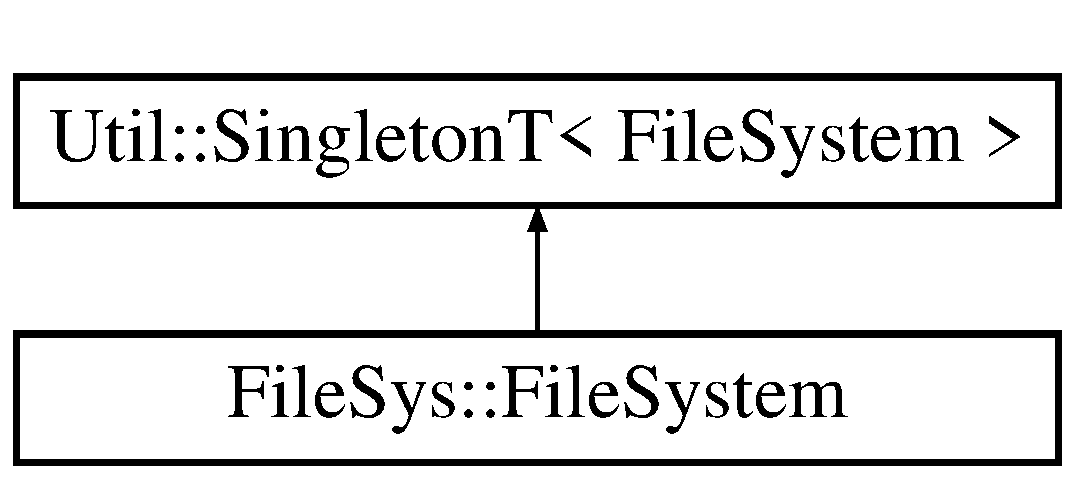
\includegraphics[height=2.000000cm]{class_file_sys_1_1_file_system}
\end{center}
\end{figure}
\subsection*{Public 成员函数}
\begin{DoxyCompactItemize}
\item 
\hyperlink{class_file_sys_1_1_node}{Node} $\ast$ \hyperlink{class_file_sys_1_1_file_system_aa5a55cf06f8ec0ba9d75c958a6cf8f12}{Root} (void) const 
\begin{DoxyCompactList}\small\item\em 获取文件系统根节点 \end{DoxyCompactList}\item 
\hypertarget{class_file_sys_1_1_file_system_a2b5ce6823a73ad89b242cae7d5bf4329}{D\-W\-O\-R\-D \hyperlink{class_file_sys_1_1_file_system_a2b5ce6823a73ad89b242cae7d5bf4329}{Total\-Size} (void)}\label{class_file_sys_1_1_file_system_a2b5ce6823a73ad89b242cae7d5bf4329}

\begin{DoxyCompactList}\small\item\em 返回文件系统的总共使用了多少内存(按字节计) \end{DoxyCompactList}\item 
\hypertarget{class_file_sys_1_1_file_system_a8f0fe8f9969ac37e840a383f370d46fc}{D\-W\-O\-R\-D \hyperlink{class_file_sys_1_1_file_system_a8f0fe8f9969ac37e840a383f370d46fc}{Capacity} (void) const }\label{class_file_sys_1_1_file_system_a8f0fe8f9969ac37e840a383f370d46fc}

\begin{DoxyCompactList}\small\item\em 返回文件系统的最大容量 \end{DoxyCompactList}\item 
\hypertarget{class_file_sys_1_1_file_system_af4c767aeb58c230de141030126271457}{bool \hyperlink{class_file_sys_1_1_file_system_af4c767aeb58c230de141030126271457}{Has\-Enough\-Space} (const D\-W\-O\-R\-D size)}\label{class_file_sys_1_1_file_system_af4c767aeb58c230de141030126271457}

\begin{DoxyCompactList}\small\item\em 查看磁盘空间是否足够容纳size个字节 \end{DoxyCompactList}\item 
\hypertarget{class_file_sys_1_1_file_system_aca5e8be14a15b85123290426ae39eb3b}{void \hyperlink{class_file_sys_1_1_file_system_aca5e8be14a15b85123290426ae39eb3b}{Accept} (\hyperlink{class_file_sys_1_1_node_visitor}{Node\-Visitor} $\ast$visitor)}\label{class_file_sys_1_1_file_system_aca5e8be14a15b85123290426ae39eb3b}

\begin{DoxyCompactList}\small\item\em 接受节点访问者访问 \end{DoxyCompactList}\item 
\hypertarget{class_file_sys_1_1_file_system_a1b9e4349d586ac1ce526f43727396190}{void \hyperlink{class_file_sys_1_1_file_system_a1b9e4349d586ac1ce526f43727396190}{Build\-Test\-File\-Tree} (void)}\label{class_file_sys_1_1_file_system_a1b9e4349d586ac1ce526f43727396190}

\begin{DoxyCompactList}\small\item\em 创建实验用文件树 \end{DoxyCompactList}\end{DoxyCompactItemize}
\subsection*{额外继承的成员函数}


\subsection{详细描述}


在文件 File\-System.\-h 第 13 行定义.



\subsection{成员函数说明}
\hypertarget{class_file_sys_1_1_file_system_aa5a55cf06f8ec0ba9d75c958a6cf8f12}{\index{File\-Sys\-::\-File\-System@{File\-Sys\-::\-File\-System}!Root@{Root}}
\index{Root@{Root}!FileSys::FileSystem@{File\-Sys\-::\-File\-System}}
\subsubsection[{Root}]{\setlength{\rightskip}{0pt plus 5cm}{\bf Node}$\ast$ File\-Sys\-::\-File\-System\-::\-Root (
\begin{DoxyParamCaption}
\item[{void}]{}
\end{DoxyParamCaption}
) const\hspace{0.3cm}{\ttfamily [inline]}}}\label{class_file_sys_1_1_file_system_aa5a55cf06f8ec0ba9d75c958a6cf8f12}


获取文件系统根节点 

\begin{DoxyReturn}{返回}
根节点 
\end{DoxyReturn}


在文件 File\-System.\-h 第 23 行定义.



该类的文档由以下文件生成\-:\begin{DoxyCompactItemize}
\item 
Virtual\-Disk\-Console/File\-System.\-h\item 
Virtual\-Disk\-Console/File\-System.\-cpp\end{DoxyCompactItemize}

\hypertarget{class_file_sys_1_1_folder_node}{\section{File\-Sys\-:\-:Folder\-Node类 参考}
\label{class_file_sys_1_1_folder_node}\index{File\-Sys\-::\-Folder\-Node@{File\-Sys\-::\-Folder\-Node}}
}
类 File\-Sys\-:\-:Folder\-Node 继承关系图\-:\begin{figure}[H]
\begin{center}
\leavevmode
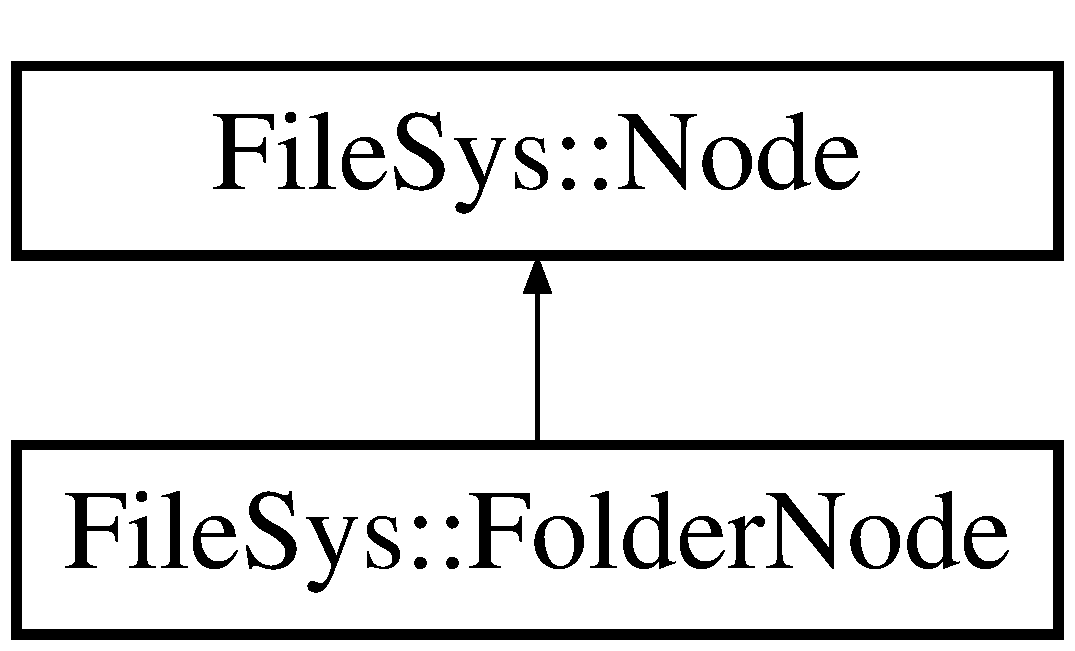
\includegraphics[height=2.000000cm]{class_file_sys_1_1_folder_node}
\end{center}
\end{figure}
\subsection*{Public 成员函数}
\begin{DoxyCompactItemize}
\item 
bool \hyperlink{class_file_sys_1_1_folder_node_a050961bdc9d98b7645bc518e215dd929}{Is\-Folder} (void) const 
\begin{DoxyCompactList}\small\item\em 是否为文件夹 \end{DoxyCompactList}\item 
virtual D\-W\-O\-R\-D \hyperlink{class_file_sys_1_1_folder_node_a6110e52309d675646c67b37e60b37ee5}{Calc\-Total\-Size} (void)
\begin{DoxyCompactList}\small\item\em 递归计算该节点子树附带数据的总大小 \end{DoxyCompactList}\item 
virtual void \hyperlink{class_file_sys_1_1_folder_node_a49bedb5a2504bdc13a86bcd38aa31ef6}{Get\-File\-List\-Output\-String} (Util\-::\-String \&output, const bool recursive=false, const bool folder\-\_\-only=false) const 
\begin{DoxyCompactList}\small\item\em 获取文件列表打印字符串 \end{DoxyCompactList}\end{DoxyCompactItemize}
\subsection*{额外继承的成员函数}


\subsection{详细描述}


在文件 Folder\-Node.\-h 第 9 行定义.



\subsection{成员函数说明}
\hypertarget{class_file_sys_1_1_folder_node_a6110e52309d675646c67b37e60b37ee5}{\index{File\-Sys\-::\-Folder\-Node@{File\-Sys\-::\-Folder\-Node}!Calc\-Total\-Size@{Calc\-Total\-Size}}
\index{Calc\-Total\-Size@{Calc\-Total\-Size}!FileSys::FolderNode@{File\-Sys\-::\-Folder\-Node}}
\subsubsection[{Calc\-Total\-Size}]{\setlength{\rightskip}{0pt plus 5cm}D\-W\-O\-R\-D File\-Sys\-::\-Folder\-Node\-::\-Calc\-Total\-Size (
\begin{DoxyParamCaption}
\item[{void}]{}
\end{DoxyParamCaption}
)\hspace{0.3cm}{\ttfamily [virtual]}}}\label{class_file_sys_1_1_folder_node_a6110e52309d675646c67b37e60b37ee5}


递归计算该节点子树附带数据的总大小 

\begin{DoxyReturn}{返回}
返回递归计算的子树附带数据大小 
\end{DoxyReturn}


重载 \hyperlink{class_file_sys_1_1_node_a6f73b0fcebfed60297a7472a954be9eb}{File\-Sys\-::\-Node} .



在文件 Folder\-Node.\-cpp 第 18 行定义.

\hypertarget{class_file_sys_1_1_folder_node_a49bedb5a2504bdc13a86bcd38aa31ef6}{\index{File\-Sys\-::\-Folder\-Node@{File\-Sys\-::\-Folder\-Node}!Get\-File\-List\-Output\-String@{Get\-File\-List\-Output\-String}}
\index{Get\-File\-List\-Output\-String@{Get\-File\-List\-Output\-String}!FileSys::FolderNode@{File\-Sys\-::\-Folder\-Node}}
\subsubsection[{Get\-File\-List\-Output\-String}]{\setlength{\rightskip}{0pt plus 5cm}void File\-Sys\-::\-Folder\-Node\-::\-Get\-File\-List\-Output\-String (
\begin{DoxyParamCaption}
\item[{Util\-::\-String \&}]{output, }
\item[{const bool}]{recursive = {\ttfamily false}, }
\item[{const bool}]{folder\-\_\-only = {\ttfamily false}}
\end{DoxyParamCaption}
) const\hspace{0.3cm}{\ttfamily [virtual]}}}\label{class_file_sys_1_1_folder_node_a49bedb5a2504bdc13a86bcd38aa31ef6}


获取文件列表打印字符串 


\begin{DoxyParams}{参数}
{\em output} & 为最终存放文件列表的字符串 \\
\hline
{\em recursive} & 指示是否是递归显示子目录与子文件 \\
\hline
\end{DoxyParams}


重载 \hyperlink{class_file_sys_1_1_node_aea400658729cd06ba5c404ed67dd5abb}{File\-Sys\-::\-Node} .



在文件 Folder\-Node.\-cpp 第 31 行定义.

\hypertarget{class_file_sys_1_1_folder_node_a050961bdc9d98b7645bc518e215dd929}{\index{File\-Sys\-::\-Folder\-Node@{File\-Sys\-::\-Folder\-Node}!Is\-Folder@{Is\-Folder}}
\index{Is\-Folder@{Is\-Folder}!FileSys::FolderNode@{File\-Sys\-::\-Folder\-Node}}
\subsubsection[{Is\-Folder}]{\setlength{\rightskip}{0pt plus 5cm}bool File\-Sys\-::\-Folder\-Node\-::\-Is\-Folder (
\begin{DoxyParamCaption}
\item[{void}]{}
\end{DoxyParamCaption}
) const\hspace{0.3cm}{\ttfamily [inline]}, {\ttfamily [virtual]}}}\label{class_file_sys_1_1_folder_node_a050961bdc9d98b7645bc518e215dd929}


是否为文件夹 

\begin{DoxyReturn}{返回}
返回是否为文件夹 
\end{DoxyReturn}


重载 \hyperlink{class_file_sys_1_1_node_ad93cc76a230827623b8fd1dbc255a9b2}{File\-Sys\-::\-Node} .



在文件 Folder\-Node.\-h 第 15 行定义.



该类的文档由以下文件生成\-:\begin{DoxyCompactItemize}
\item 
Virtual\-Disk\-Console/Folder\-Node.\-h\item 
Virtual\-Disk\-Console/Folder\-Node.\-cpp\end{DoxyCompactItemize}

\hypertarget{class_util_1_1_link_list_t_1_1_iterator}{\section{Util\-:\-:Link\-List\-T$<$ T $>$\-:\-:Iterator类 参考}
\label{class_util_1_1_link_list_t_1_1_iterator}\index{Util\-::\-Link\-List\-T$<$ T $>$\-::\-Iterator@{Util\-::\-Link\-List\-T$<$ T $>$\-::\-Iterator}}
}
\subsection*{Public 成员函数}
\begin{DoxyCompactItemize}
\item 
\hypertarget{class_util_1_1_link_list_t_1_1_iterator_a6f172ac2f8e895787b0f9b50dc8e2b3a}{{\bfseries Iterator} (\hyperlink{class_util_1_1_link_list_t}{Link\-List\-T} $\ast$list)}\label{class_util_1_1_link_list_t_1_1_iterator_a6f172ac2f8e895787b0f9b50dc8e2b3a}

\item 
\hypertarget{class_util_1_1_link_list_t_1_1_iterator_a0da84afeafd99c0f0a07f07982becb68}{{\bfseries Iterator} (\hyperlink{class_util_1_1_link_list_t}{Link\-List\-T} $\ast$list, \hyperlink{class_util_1_1_link_list_t_1_1_link_node}{Link\-Node} $\ast$node)}\label{class_util_1_1_link_list_t_1_1_iterator_a0da84afeafd99c0f0a07f07982becb68}

\item 
\hypertarget{class_util_1_1_link_list_t_1_1_iterator_ad0e8fcdaeebf2741f48abf34dd9aa0e4}{{\bfseries Iterator} (const \hyperlink{class_util_1_1_link_list_t_1_1_iterator}{Iterator} \&it)}\label{class_util_1_1_link_list_t_1_1_iterator_ad0e8fcdaeebf2741f48abf34dd9aa0e4}

\item 
\hypertarget{class_util_1_1_link_list_t_1_1_iterator_a37319d14c5b70bf9d5387f7ce5dc8d58}{void \hyperlink{class_util_1_1_link_list_t_1_1_iterator_a37319d14c5b70bf9d5387f7ce5dc8d58}{Move\-First} (void)}\label{class_util_1_1_link_list_t_1_1_iterator_a37319d14c5b70bf9d5387f7ce5dc8d58}

\begin{DoxyCompactList}\small\item\em 将迭代器重置为链表首 \end{DoxyCompactList}\item 
\hypertarget{class_util_1_1_link_list_t_1_1_iterator_a445d1378a5f43e89f76d34698a8d6260}{void \hyperlink{class_util_1_1_link_list_t_1_1_iterator_a445d1378a5f43e89f76d34698a8d6260}{Move\-Last} (void)}\label{class_util_1_1_link_list_t_1_1_iterator_a445d1378a5f43e89f76d34698a8d6260}

\begin{DoxyCompactList}\small\item\em 将迭代器移动到最后一个元素 \end{DoxyCompactList}\item 
bool \hyperlink{class_util_1_1_link_list_t_1_1_iterator_a3021df9a0b22d50e71ec451f860fb627}{Has\-Next} (void) const 
\begin{DoxyCompactList}\small\item\em 是否还有下一个元素 \end{DoxyCompactList}\item 
T \& \hyperlink{class_util_1_1_link_list_t_1_1_iterator_a2dd085a65afcd15667c078446fc712aa}{Next} (void)
\begin{DoxyCompactList}\small\item\em 返回当前元素,并移动到下一个元素 \end{DoxyCompactList}\item 
\hypertarget{class_util_1_1_link_list_t_1_1_iterator_a614c699dcbbc7b9cb2c41cc31d545d2e}{T \& {\bfseries Data} (void)}\label{class_util_1_1_link_list_t_1_1_iterator_a614c699dcbbc7b9cb2c41cc31d545d2e}

\item 
\hypertarget{class_util_1_1_link_list_t_1_1_iterator_ad9194119d4ffc0b90cecc79b8cd50bce}{const T \& {\bfseries Data} (void) const }\label{class_util_1_1_link_list_t_1_1_iterator_ad9194119d4ffc0b90cecc79b8cd50bce}

\item 
\hypertarget{class_util_1_1_link_list_t_1_1_iterator_a4513474b857dbba6c3123fec8672437d}{T \& {\bfseries operator$\ast$} ()}\label{class_util_1_1_link_list_t_1_1_iterator_a4513474b857dbba6c3123fec8672437d}

\item 
\hypertarget{class_util_1_1_link_list_t_1_1_iterator_a0a1eca838c89167bd079b7fbc1cb160b}{const T \& {\bfseries operator$\ast$} () const }\label{class_util_1_1_link_list_t_1_1_iterator_a0a1eca838c89167bd079b7fbc1cb160b}

\item 
\hypertarget{class_util_1_1_link_list_t_1_1_iterator_a25bb77786e573ec7db58c38bf9f06e9f}{bool {\bfseries operator==} (const \hyperlink{class_util_1_1_link_list_t_1_1_iterator}{Iterator} \&rhs)}\label{class_util_1_1_link_list_t_1_1_iterator_a25bb77786e573ec7db58c38bf9f06e9f}

\item 
\hypertarget{class_util_1_1_link_list_t_1_1_iterator_a4a9c03afdc8132f21d6df8ad8a425a3b}{bool {\bfseries operator!=} (const \hyperlink{class_util_1_1_link_list_t_1_1_iterator}{Iterator} \&rhs)}\label{class_util_1_1_link_list_t_1_1_iterator_a4a9c03afdc8132f21d6df8ad8a425a3b}

\item 
\hypertarget{class_util_1_1_link_list_t_1_1_iterator_a3b2e243b8b75ad1c77fa501ac604cc4b}{\hyperlink{class_util_1_1_link_list_t_1_1_iterator}{Iterator} \& {\bfseries operator=} (const \hyperlink{class_util_1_1_link_list_t_1_1_iterator}{Iterator} \&rhs)}\label{class_util_1_1_link_list_t_1_1_iterator_a3b2e243b8b75ad1c77fa501ac604cc4b}

\end{DoxyCompactItemize}
\subsection*{Protected 成员函数}
\begin{DoxyCompactItemize}
\item 
\hyperlink{class_util_1_1_link_list_t_1_1_link_node}{Link\-Node} $\ast$ \hyperlink{class_util_1_1_link_list_t_1_1_iterator_ab4eb0a7e476bc9b7948ce8fc4ac75f8e}{Curr\-Node} (void) const 
\begin{DoxyCompactList}\small\item\em 返回迭代器指代的当前结点 \end{DoxyCompactList}\item 
void \hyperlink{class_util_1_1_link_list_t_1_1_iterator_af4f3c41800abeb38949f49fbfe0b27d3}{Curr\-Node} (\hyperlink{class_util_1_1_link_list_t_1_1_link_node}{Link\-Node} $\ast$node)
\begin{DoxyCompactList}\small\item\em 设置当前迭代器结点指针 \end{DoxyCompactList}\end{DoxyCompactItemize}
\subsection*{友元}
\begin{DoxyCompactItemize}
\item 
\hypertarget{class_util_1_1_link_list_t_1_1_iterator_a4b02bb15a329bfedcc19f00342bb4b49}{class {\bfseries Link\-List\-T}}\label{class_util_1_1_link_list_t_1_1_iterator_a4b02bb15a329bfedcc19f00342bb4b49}

\end{DoxyCompactItemize}


\subsection{详细描述}
\subsubsection*{template$<$typename T$>$class Util\-::\-Link\-List\-T$<$ T $>$\-::\-Iterator}



在文件 Link\-List.\-h 第 502 行定义.



\subsection{成员函数说明}
\hypertarget{class_util_1_1_link_list_t_1_1_iterator_ab4eb0a7e476bc9b7948ce8fc4ac75f8e}{\index{Util\-::\-Link\-List\-T\-::\-Iterator@{Util\-::\-Link\-List\-T\-::\-Iterator}!Curr\-Node@{Curr\-Node}}
\index{Curr\-Node@{Curr\-Node}!Util::LinkListT::Iterator@{Util\-::\-Link\-List\-T\-::\-Iterator}}
\subsubsection[{Curr\-Node}]{\setlength{\rightskip}{0pt plus 5cm}template$<$typename T$>$ {\bf Link\-Node}$\ast$ {\bf Util\-::\-Link\-List\-T}$<$ T $>$\-::Iterator\-::\-Curr\-Node (
\begin{DoxyParamCaption}
\item[{void}]{}
\end{DoxyParamCaption}
) const\hspace{0.3cm}{\ttfamily [inline]}, {\ttfamily [protected]}}}\label{class_util_1_1_link_list_t_1_1_iterator_ab4eb0a7e476bc9b7948ce8fc4ac75f8e}


返回迭代器指代的当前结点 

\begin{DoxyReturn}{返回}
当前结点指针 
\end{DoxyReturn}
\begin{DoxyRemark}{备注}
仅供内部调用 
\end{DoxyRemark}


在文件 Link\-List.\-h 第 614 行定义.

\hypertarget{class_util_1_1_link_list_t_1_1_iterator_af4f3c41800abeb38949f49fbfe0b27d3}{\index{Util\-::\-Link\-List\-T\-::\-Iterator@{Util\-::\-Link\-List\-T\-::\-Iterator}!Curr\-Node@{Curr\-Node}}
\index{Curr\-Node@{Curr\-Node}!Util::LinkListT::Iterator@{Util\-::\-Link\-List\-T\-::\-Iterator}}
\subsubsection[{Curr\-Node}]{\setlength{\rightskip}{0pt plus 5cm}template$<$typename T$>$ void {\bf Util\-::\-Link\-List\-T}$<$ T $>$\-::Iterator\-::\-Curr\-Node (
\begin{DoxyParamCaption}
\item[{{\bf Link\-Node} $\ast$}]{node}
\end{DoxyParamCaption}
)\hspace{0.3cm}{\ttfamily [inline]}, {\ttfamily [protected]}}}\label{class_util_1_1_link_list_t_1_1_iterator_af4f3c41800abeb38949f49fbfe0b27d3}


设置当前迭代器结点指针 


\begin{DoxyParams}{参数}
{\em node} & 要设置的结点指针 \\
\hline
\end{DoxyParams}
\begin{DoxyReturn}{返回}
void 
\end{DoxyReturn}
\begin{DoxyRemark}{备注}
仅供内部调用 
\end{DoxyRemark}


在文件 Link\-List.\-h 第 621 行定义.

\hypertarget{class_util_1_1_link_list_t_1_1_iterator_a3021df9a0b22d50e71ec451f860fb627}{\index{Util\-::\-Link\-List\-T\-::\-Iterator@{Util\-::\-Link\-List\-T\-::\-Iterator}!Has\-Next@{Has\-Next}}
\index{Has\-Next@{Has\-Next}!Util::LinkListT::Iterator@{Util\-::\-Link\-List\-T\-::\-Iterator}}
\subsubsection[{Has\-Next}]{\setlength{\rightskip}{0pt plus 5cm}template$<$typename T$>$ bool {\bf Util\-::\-Link\-List\-T}$<$ T $>$\-::Iterator\-::\-Has\-Next (
\begin{DoxyParamCaption}
\item[{void}]{}
\end{DoxyParamCaption}
) const\hspace{0.3cm}{\ttfamily [inline]}}}\label{class_util_1_1_link_list_t_1_1_iterator_a3021df9a0b22d50e71ec451f860fb627}


是否还有下一个元素 


\begin{DoxyRetVals}{返回值}
{\em true} & 还有下一个元素 \\
\hline
{\em false} & 没有下一个元素 \\
\hline
\end{DoxyRetVals}


在文件 Link\-List.\-h 第 550 行定义.

\hypertarget{class_util_1_1_link_list_t_1_1_iterator_a2dd085a65afcd15667c078446fc712aa}{\index{Util\-::\-Link\-List\-T\-::\-Iterator@{Util\-::\-Link\-List\-T\-::\-Iterator}!Next@{Next}}
\index{Next@{Next}!Util::LinkListT::Iterator@{Util\-::\-Link\-List\-T\-::\-Iterator}}
\subsubsection[{Next}]{\setlength{\rightskip}{0pt plus 5cm}template$<$typename T$>$ T\& {\bf Util\-::\-Link\-List\-T}$<$ T $>$\-::Iterator\-::\-Next (
\begin{DoxyParamCaption}
\item[{void}]{}
\end{DoxyParamCaption}
)\hspace{0.3cm}{\ttfamily [inline]}}}\label{class_util_1_1_link_list_t_1_1_iterator_a2dd085a65afcd15667c078446fc712aa}


返回当前元素,并移动到下一个元素 

\begin{DoxyReturn}{返回}
当前元素值 
\end{DoxyReturn}


在文件 Link\-List.\-h 第 556 行定义.



该类的文档由以下文件生成\-:\begin{DoxyCompactItemize}
\item 
Virtual\-Disk\-Console/Link\-List.\-h\end{DoxyCompactItemize}

\hypertarget{class_lexer_sys_1_1_lexer}{\section{Lexer\-Sys\-:\-:Lexer类 参考}
\label{class_lexer_sys_1_1_lexer}\index{Lexer\-Sys\-::\-Lexer@{Lexer\-Sys\-::\-Lexer}}
}
\subsection*{Public 类型}
\begin{DoxyCompactItemize}
\item 
enum {\bfseries Lexer\-State} \{ {\bfseries L\-O\-A\-D\-E\-D\-\_\-\-S\-T\-A\-T\-E} = 1, 
{\bfseries U\-N\-L\-O\-A\-D\-E\-D\-\_\-\-S\-T\-A\-T\-E}, 
{\bfseries A\-N\-A\-L\-Y\-S\-I\-S\-E\-D\-\_\-\-S\-T\-A\-T\-E}
 \}
\end{DoxyCompactItemize}
\subsection*{Public 成员函数}
\begin{DoxyCompactItemize}
\item 
virtual void \hyperlink{class_lexer_sys_1_1_lexer_ac3a3c82b210ed2be7f1996180c124176}{Set\-String} (const Util\-::\-String \&str)
\begin{DoxyCompactList}\small\item\em 设置需要分析的字符串 \end{DoxyCompactList}\item 
virtual \hyperlink{class_lexer_sys_1_1_token}{Token} \& \hyperlink{class_lexer_sys_1_1_lexer_aa55e3ab31601792897465e2772eb255d}{Get\-Command\-Token} (void)
\begin{DoxyCompactList}\small\item\em 获得命令头 \end{DoxyCompactList}\item 
virtual \hyperlink{class_util_1_1_link_list_t}{Util\-::\-Link\-List\-T}$<$ \hyperlink{class_lexer_sys_1_1_token}{Token} $>$ \& \hyperlink{class_lexer_sys_1_1_lexer_a97215f1bea5d215e1260efb7a001c738}{Get\-Command\-Options} (void)
\begin{DoxyCompactList}\small\item\em 获得命令选项 \end{DoxyCompactList}\item 
virtual \hyperlink{class_util_1_1_link_list_t}{Util\-::\-Link\-List\-T}\\*
$<$ \hyperlink{class_lexer_sys_1_1_search_path}{Search\-Path} $>$ \& \hyperlink{class_lexer_sys_1_1_lexer_aead2ffdb9f57cc2cf582611b97557223}{Get\-Command\-Paths} (void)
\begin{DoxyCompactList}\small\item\em 获得命令路径列表 \end{DoxyCompactList}\item 
\hypertarget{class_lexer_sys_1_1_lexer_aea64d5beaaaa4339b2c2b152a0c420bf}{virtual void \hyperlink{class_lexer_sys_1_1_lexer_aea64d5beaaaa4339b2c2b152a0c420bf}{Analysis} (void)}\label{class_lexer_sys_1_1_lexer_aea64d5beaaaa4339b2c2b152a0c420bf}

\begin{DoxyCompactList}\small\item\em 分析所设置的字符串,从中分析出各种token \end{DoxyCompactList}\item 
\hypertarget{class_lexer_sys_1_1_lexer_a8921b421de22b3f7ef44cfadfe1e4dc7}{virtual void \hyperlink{class_lexer_sys_1_1_lexer_a8921b421de22b3f7ef44cfadfe1e4dc7}{Clear} (void)}\label{class_lexer_sys_1_1_lexer_a8921b421de22b3f7ef44cfadfe1e4dc7}

\begin{DoxyCompactList}\small\item\em 清空解析器内容供下次再次分析 \end{DoxyCompactList}\end{DoxyCompactItemize}
\subsection*{Protected 成员函数}
\begin{DoxyCompactItemize}
\item 
Util\-::\-String \hyperlink{class_lexer_sys_1_1_lexer_a5a838652fece37b063d6e71efb87c1c6}{Analysis\-Cmd\-Head} (const Util\-::\-String \&str)
\begin{DoxyCompactList}\small\item\em 从要分析的字符串中提取命令头 \end{DoxyCompactList}\item 
Util\-::\-String \hyperlink{class_lexer_sys_1_1_lexer_ae143c5f4c628b05b7bcc41d1f79cd6e6}{Analysis\-Cmd\-Options} (const Util\-::\-String \&str)
\begin{DoxyCompactList}\small\item\em 从要分析的字符串中提取命令选项 \end{DoxyCompactList}\item 
Util\-::\-String \hyperlink{class_lexer_sys_1_1_lexer_a3d7bd63169463c2bb476656bb46fb144}{Analysis\-Cmd\-Paths} (const Util\-::\-String \&str)
\begin{DoxyCompactList}\small\item\em 从要分析的字符串中提取命令路径 \end{DoxyCompactList}\end{DoxyCompactItemize}


\subsection{详细描述}


在文件 Lexer.\-h 第 16 行定义.



\subsection{成员函数说明}
\hypertarget{class_lexer_sys_1_1_lexer_a5a838652fece37b063d6e71efb87c1c6}{\index{Lexer\-Sys\-::\-Lexer@{Lexer\-Sys\-::\-Lexer}!Analysis\-Cmd\-Head@{Analysis\-Cmd\-Head}}
\index{Analysis\-Cmd\-Head@{Analysis\-Cmd\-Head}!LexerSys::Lexer@{Lexer\-Sys\-::\-Lexer}}
\subsubsection[{Analysis\-Cmd\-Head}]{\setlength{\rightskip}{0pt plus 5cm}Util\-::\-String Lexer\-Sys\-::\-Lexer\-::\-Analysis\-Cmd\-Head (
\begin{DoxyParamCaption}
\item[{const Util\-::\-String \&}]{str}
\end{DoxyParamCaption}
)\hspace{0.3cm}{\ttfamily [protected]}}}\label{class_lexer_sys_1_1_lexer_a5a838652fece37b063d6e71efb87c1c6}


从要分析的字符串中提取命令头 

\begin{DoxyRemark}{备注}
仅供内部调用函数 
\end{DoxyRemark}


在文件 Lexer.\-cpp 第 46 行定义.

\hypertarget{class_lexer_sys_1_1_lexer_ae143c5f4c628b05b7bcc41d1f79cd6e6}{\index{Lexer\-Sys\-::\-Lexer@{Lexer\-Sys\-::\-Lexer}!Analysis\-Cmd\-Options@{Analysis\-Cmd\-Options}}
\index{Analysis\-Cmd\-Options@{Analysis\-Cmd\-Options}!LexerSys::Lexer@{Lexer\-Sys\-::\-Lexer}}
\subsubsection[{Analysis\-Cmd\-Options}]{\setlength{\rightskip}{0pt plus 5cm}Util\-::\-String Lexer\-Sys\-::\-Lexer\-::\-Analysis\-Cmd\-Options (
\begin{DoxyParamCaption}
\item[{const Util\-::\-String \&}]{str}
\end{DoxyParamCaption}
)\hspace{0.3cm}{\ttfamily [protected]}}}\label{class_lexer_sys_1_1_lexer_ae143c5f4c628b05b7bcc41d1f79cd6e6}


从要分析的字符串中提取命令选项 

\begin{DoxyRemark}{备注}
仅供内部调用函数 
\end{DoxyRemark}


在文件 Lexer.\-cpp 第 70 行定义.

\hypertarget{class_lexer_sys_1_1_lexer_a3d7bd63169463c2bb476656bb46fb144}{\index{Lexer\-Sys\-::\-Lexer@{Lexer\-Sys\-::\-Lexer}!Analysis\-Cmd\-Paths@{Analysis\-Cmd\-Paths}}
\index{Analysis\-Cmd\-Paths@{Analysis\-Cmd\-Paths}!LexerSys::Lexer@{Lexer\-Sys\-::\-Lexer}}
\subsubsection[{Analysis\-Cmd\-Paths}]{\setlength{\rightskip}{0pt plus 5cm}Util\-::\-String Lexer\-Sys\-::\-Lexer\-::\-Analysis\-Cmd\-Paths (
\begin{DoxyParamCaption}
\item[{const Util\-::\-String \&}]{str}
\end{DoxyParamCaption}
)\hspace{0.3cm}{\ttfamily [protected]}}}\label{class_lexer_sys_1_1_lexer_a3d7bd63169463c2bb476656bb46fb144}


从要分析的字符串中提取命令路径 

\begin{DoxyRemark}{备注}
仅供内部调用函数 
\end{DoxyRemark}


在文件 Lexer.\-cpp 第 120 行定义.

\hypertarget{class_lexer_sys_1_1_lexer_a97215f1bea5d215e1260efb7a001c738}{\index{Lexer\-Sys\-::\-Lexer@{Lexer\-Sys\-::\-Lexer}!Get\-Command\-Options@{Get\-Command\-Options}}
\index{Get\-Command\-Options@{Get\-Command\-Options}!LexerSys::Lexer@{Lexer\-Sys\-::\-Lexer}}
\subsubsection[{Get\-Command\-Options}]{\setlength{\rightskip}{0pt plus 5cm}virtual {\bf Util\-::\-Link\-List\-T}$<${\bf Token}$>$\& Lexer\-Sys\-::\-Lexer\-::\-Get\-Command\-Options (
\begin{DoxyParamCaption}
\item[{void}]{}
\end{DoxyParamCaption}
)\hspace{0.3cm}{\ttfamily [inline]}, {\ttfamily [virtual]}}}\label{class_lexer_sys_1_1_lexer_a97215f1bea5d215e1260efb7a001c738}


获得命令选项 

\begin{DoxyReturn}{返回}
命令选项列表 
\end{DoxyReturn}


在文件 Lexer.\-h 第 45 行定义.

\hypertarget{class_lexer_sys_1_1_lexer_aead2ffdb9f57cc2cf582611b97557223}{\index{Lexer\-Sys\-::\-Lexer@{Lexer\-Sys\-::\-Lexer}!Get\-Command\-Paths@{Get\-Command\-Paths}}
\index{Get\-Command\-Paths@{Get\-Command\-Paths}!LexerSys::Lexer@{Lexer\-Sys\-::\-Lexer}}
\subsubsection[{Get\-Command\-Paths}]{\setlength{\rightskip}{0pt plus 5cm}virtual {\bf Util\-::\-Link\-List\-T}$<${\bf Search\-Path}$>$\& Lexer\-Sys\-::\-Lexer\-::\-Get\-Command\-Paths (
\begin{DoxyParamCaption}
\item[{void}]{}
\end{DoxyParamCaption}
)\hspace{0.3cm}{\ttfamily [inline]}, {\ttfamily [virtual]}}}\label{class_lexer_sys_1_1_lexer_aead2ffdb9f57cc2cf582611b97557223}


获得命令路径列表 

\begin{DoxyReturn}{返回}
获得命令路径列表 
\end{DoxyReturn}


在文件 Lexer.\-h 第 51 行定义.

\hypertarget{class_lexer_sys_1_1_lexer_aa55e3ab31601792897465e2772eb255d}{\index{Lexer\-Sys\-::\-Lexer@{Lexer\-Sys\-::\-Lexer}!Get\-Command\-Token@{Get\-Command\-Token}}
\index{Get\-Command\-Token@{Get\-Command\-Token}!LexerSys::Lexer@{Lexer\-Sys\-::\-Lexer}}
\subsubsection[{Get\-Command\-Token}]{\setlength{\rightskip}{0pt plus 5cm}virtual {\bf Token}\& Lexer\-Sys\-::\-Lexer\-::\-Get\-Command\-Token (
\begin{DoxyParamCaption}
\item[{void}]{}
\end{DoxyParamCaption}
)\hspace{0.3cm}{\ttfamily [inline]}, {\ttfamily [virtual]}}}\label{class_lexer_sys_1_1_lexer_aa55e3ab31601792897465e2772eb255d}


获得命令头 

\begin{DoxyReturn}{返回}
命令头符号 
\end{DoxyReturn}


在文件 Lexer.\-h 第 39 行定义.

\hypertarget{class_lexer_sys_1_1_lexer_ac3a3c82b210ed2be7f1996180c124176}{\index{Lexer\-Sys\-::\-Lexer@{Lexer\-Sys\-::\-Lexer}!Set\-String@{Set\-String}}
\index{Set\-String@{Set\-String}!LexerSys::Lexer@{Lexer\-Sys\-::\-Lexer}}
\subsubsection[{Set\-String}]{\setlength{\rightskip}{0pt plus 5cm}void Lexer\-Sys\-::\-Lexer\-::\-Set\-String (
\begin{DoxyParamCaption}
\item[{const Util\-::\-String \&}]{str}
\end{DoxyParamCaption}
)\hspace{0.3cm}{\ttfamily [virtual]}}}\label{class_lexer_sys_1_1_lexer_ac3a3c82b210ed2be7f1996180c124176}


设置需要分析的字符串 


\begin{DoxyParams}{参数}
{\em str} & 需要分析的字符串 \\
\hline
\end{DoxyParams}


在文件 Lexer.\-cpp 第 19 行定义.



该类的文档由以下文件生成\-:\begin{DoxyCompactItemize}
\item 
Virtual\-Disk\-Console/Lexer.\-h\item 
Virtual\-Disk\-Console/Lexer.\-cpp\end{DoxyCompactItemize}

\hypertarget{class_util_1_1_link_list_t}{\section{Util\-:\-:Link\-List\-T$<$ T $>$ 模板类 参考}
\label{class_util_1_1_link_list_t}\index{Util\-::\-Link\-List\-T$<$ T $>$@{Util\-::\-Link\-List\-T$<$ T $>$}}
}
\subsection*{类}
\begin{DoxyCompactItemize}
\item 
class \hyperlink{class_util_1_1_link_list_t_1_1_iterator}{Iterator}
\item 
class \hyperlink{class_util_1_1_link_list_t_1_1_link_node}{Link\-Node}
\end{DoxyCompactItemize}
\subsection*{Public 成员函数}
\begin{DoxyCompactItemize}
\item 
\hypertarget{class_util_1_1_link_list_t_a60b5fa84c6795eb44df4f8d367272c79}{\hyperlink{class_util_1_1_link_list_t_a60b5fa84c6795eb44df4f8d367272c79}{Link\-List\-T} ()}\label{class_util_1_1_link_list_t_a60b5fa84c6795eb44df4f8d367272c79}

\begin{DoxyCompactList}\small\item\em 默认构造函数 \end{DoxyCompactList}\item 
\hypertarget{class_util_1_1_link_list_t_a3e7e079ee9b667250aad21c057e2c3ab}{\hyperlink{class_util_1_1_link_list_t_a3e7e079ee9b667250aad21c057e2c3ab}{Link\-List\-T} (const \hyperlink{class_util_1_1_link_list_t}{Link\-List\-T} \&list)}\label{class_util_1_1_link_list_t_a3e7e079ee9b667250aad21c057e2c3ab}

\begin{DoxyCompactList}\small\item\em 拷贝构造函数 \end{DoxyCompactList}\item 
\hypertarget{class_util_1_1_link_list_t_aaf952435048591b3c8de20f4d2363cdc}{\hyperlink{class_util_1_1_link_list_t_aaf952435048591b3c8de20f4d2363cdc}{$\sim$\-Link\-List\-T} ()}\label{class_util_1_1_link_list_t_aaf952435048591b3c8de20f4d2363cdc}

\begin{DoxyCompactList}\small\item\em 析构函数 \end{DoxyCompactList}\item 
\hyperlink{class_util_1_1_link_list_t_1_1_link_node}{Link\-Node} $\ast$ \hyperlink{class_util_1_1_link_list_t_a1bce3005e2fa80505d554725aa39ea7b}{Head} (void)
\begin{DoxyCompactList}\small\item\em 返回头结点指针 \end{DoxyCompactList}\item 
const \hyperlink{class_util_1_1_link_list_t_1_1_link_node}{Link\-Node} $\ast$ \hyperlink{class_util_1_1_link_list_t_a0eacfdc2967ebc4398c256045b42c9e0}{Head} (void) const 
\begin{DoxyCompactList}\small\item\em 返回头结点指针 \end{DoxyCompactList}\item 
\hyperlink{class_util_1_1_link_list_t_1_1_link_node}{Link\-Node} $\ast$ \hyperlink{class_util_1_1_link_list_t_a1dc4db8985e3b8d4d3a70940cbaf91cd}{Tail} (void)
\begin{DoxyCompactList}\small\item\em 返回尾结点指针 \end{DoxyCompactList}\item 
const \hyperlink{class_util_1_1_link_list_t_1_1_link_node}{Link\-Node} $\ast$ \hyperlink{class_util_1_1_link_list_t_a3de4674fbd5e53c7d15234ecb6a94fcd}{Tail} (void) const 
\begin{DoxyCompactList}\small\item\em 返回尾结点指针 \end{DoxyCompactList}\item 
int \hyperlink{class_util_1_1_link_list_t_a67b0960b3562bf628e3dac416591193e}{Count} (void) const 
\begin{DoxyCompactList}\small\item\em 返回链表中结点数 \end{DoxyCompactList}\item 
\hypertarget{class_util_1_1_link_list_t_a1bc012ec7cd5c67ca0451d2106a21d68}{T \& {\bfseries Front} (void)}\label{class_util_1_1_link_list_t_a1bc012ec7cd5c67ca0451d2106a21d68}

\item 
\hypertarget{class_util_1_1_link_list_t_a43ce5d976e787777abf2cdd380eb43e8}{const T \& {\bfseries Front} (void) const }\label{class_util_1_1_link_list_t_a43ce5d976e787777abf2cdd380eb43e8}

\item 
\hypertarget{class_util_1_1_link_list_t_a50a6be84ff3763b8905065dd0b4ea3d2}{T \& {\bfseries Back} (void)}\label{class_util_1_1_link_list_t_a50a6be84ff3763b8905065dd0b4ea3d2}

\item 
\hypertarget{class_util_1_1_link_list_t_a1e84d4db095eea6176e69033fec1b7f1}{const T \& {\bfseries Back} (void) const }\label{class_util_1_1_link_list_t_a1e84d4db095eea6176e69033fec1b7f1}

\item 
void \hyperlink{class_util_1_1_link_list_t_a23cd50293429437d6b3695bad16ce846}{Push\-Front} (const T \&data)
\begin{DoxyCompactList}\small\item\em 从前端插入一个以data为数据的结点 \end{DoxyCompactList}\item 
void \hyperlink{class_util_1_1_link_list_t_a3bbe08d8e419e3fc7ce714994a0f7505}{Push\-Back} (const T \&data)
\begin{DoxyCompactList}\small\item\em 从后端插入一个以data为数据的结点 \end{DoxyCompactList}\item 
\hypertarget{class_util_1_1_link_list_t_a035b833be025ca3c1dbf9e1e740ffaeb}{void \hyperlink{class_util_1_1_link_list_t_a035b833be025ca3c1dbf9e1e740ffaeb}{Pop\-Front} (void)}\label{class_util_1_1_link_list_t_a035b833be025ca3c1dbf9e1e740ffaeb}

\begin{DoxyCompactList}\small\item\em 销毁头部一个结点 \end{DoxyCompactList}\item 
\hypertarget{class_util_1_1_link_list_t_ad7bba2fe869cd01bae4ea14e3af31d7e}{void \hyperlink{class_util_1_1_link_list_t_ad7bba2fe869cd01bae4ea14e3af31d7e}{Pop\-Back} (void)}\label{class_util_1_1_link_list_t_ad7bba2fe869cd01bae4ea14e3af31d7e}

\begin{DoxyCompactList}\small\item\em 销毁尾部一个结点 \end{DoxyCompactList}\item 
\hyperlink{class_util_1_1_link_list_t_1_1_link_node}{Link\-Node} $\ast$ \hyperlink{class_util_1_1_link_list_t_a7a37440fafe515f7d4a41f1092455a5c}{Erase} (\hyperlink{class_util_1_1_link_list_t_1_1_link_node}{Link\-Node} $\ast$node)
\begin{DoxyCompactList}\small\item\em 删除掉所指定的结点 \end{DoxyCompactList}\item 
\hypertarget{class_util_1_1_link_list_t_ad9defc05d4cc572f91d3dcc901670987}{T \& \hyperlink{class_util_1_1_link_list_t_ad9defc05d4cc572f91d3dcc901670987}{At} (const int i)}\label{class_util_1_1_link_list_t_ad9defc05d4cc572f91d3dcc901670987}

\begin{DoxyCompactList}\small\item\em 获取在i处的元素 \end{DoxyCompactList}\item 
\hypertarget{class_util_1_1_link_list_t_a102945173d8f6b7af8d60b9b1ea70749}{const T \& {\bfseries At} (const int i) const }\label{class_util_1_1_link_list_t_a102945173d8f6b7af8d60b9b1ea70749}

\item 
void \hyperlink{class_util_1_1_link_list_t_a5eec94fcd813720cbc1d1705386b44b6}{Insert} (const int i, const T \&data)
\begin{DoxyCompactList}\small\item\em 在位置i处插入数据 data \end{DoxyCompactList}\item 
void \hyperlink{class_util_1_1_link_list_t_a61b8ac3151b64b43d83a39e214ca2fcf}{Delete\-At} (const int i)
\begin{DoxyCompactList}\small\item\em 删除索引所指定的节点 \end{DoxyCompactList}\item 
bool \hyperlink{class_util_1_1_link_list_t_a8a6e3578116db560b1671d031f68acfe}{Is\-Empty} (void) const 
\begin{DoxyCompactList}\small\item\em 返回链表是否为空 \end{DoxyCompactList}\item 
\hypertarget{class_util_1_1_link_list_t_a756f91eb4237ffd79b6c4d04845ed1ea}{void \hyperlink{class_util_1_1_link_list_t_a756f91eb4237ffd79b6c4d04845ed1ea}{Clear} (void)}\label{class_util_1_1_link_list_t_a756f91eb4237ffd79b6c4d04845ed1ea}

\begin{DoxyCompactList}\small\item\em 清空链表中的所有结点 \end{DoxyCompactList}\item 
void \hyperlink{class_util_1_1_link_list_t_a8af74682abd66f3e337bbf1a82670367}{Clone} (const \hyperlink{class_util_1_1_link_list_t}{Link\-List\-T} \&list)
\begin{DoxyCompactList}\small\item\em 拷贝另一个链表 \end{DoxyCompactList}\item 
\hyperlink{class_util_1_1_link_list_t}{Link\-List\-T} \& \hyperlink{class_util_1_1_link_list_t_acc648d5a22f4aec6ae93caccc2c849bb}{Append} (const \hyperlink{class_util_1_1_link_list_t}{Link\-List\-T} \&list)
\begin{DoxyCompactList}\small\item\em 在当前链表处附加一个链表 \end{DoxyCompactList}\item 
void \hyperlink{class_util_1_1_link_list_t_a8c70c54bfd46772be4047634d7c01f1c}{Swap} (\hyperlink{class_util_1_1_link_list_t}{Link\-List\-T} \&list)
\begin{DoxyCompactList}\small\item\em 交换两个链表 \end{DoxyCompactList}\item 
\hypertarget{class_util_1_1_link_list_t_a3317850f32881fb26c819b795d7703d8}{\hyperlink{class_util_1_1_link_list_t}{Link\-List\-T} \& \hyperlink{class_util_1_1_link_list_t_a3317850f32881fb26c819b795d7703d8}{operator=} (const \hyperlink{class_util_1_1_link_list_t}{Link\-List\-T} \&rhs)}\label{class_util_1_1_link_list_t_a3317850f32881fb26c819b795d7703d8}

\begin{DoxyCompactList}\small\item\em 赋值运算符重载 \end{DoxyCompactList}\item 
\hyperlink{class_util_1_1_link_list_t_1_1_iterator}{Iterator} \hyperlink{class_util_1_1_link_list_t_ac504a12593f858abff816274f9712c20}{Begin} (void)
\begin{DoxyCompactList}\small\item\em 返回指向链表起始迭代器 \end{DoxyCompactList}\item 
\hyperlink{class_util_1_1_link_list_t_1_1_iterator}{Iterator} \hyperlink{class_util_1_1_link_list_t_a3994d72d98f331f617362441717b3cb1}{End} (void)
\begin{DoxyCompactList}\small\item\em 返回指向链表结尾的迭代器 \end{DoxyCompactList}\item 
\hyperlink{class_util_1_1_link_list_t_1_1_iterator}{Iterator} \hyperlink{class_util_1_1_link_list_t_a79ef572c787c52627a865bba3d8698f8}{Erase} (\hyperlink{class_util_1_1_link_list_t_1_1_iterator}{Iterator} \&it)
\begin{DoxyCompactList}\small\item\em 删除迭代器所指向结点 \end{DoxyCompactList}\end{DoxyCompactItemize}


\subsection{详细描述}
\subsubsection*{template$<$typename T$>$class Util\-::\-Link\-List\-T$<$ T $>$}



在文件 Link\-List.\-h 第 8 行定义.



\subsection{成员函数说明}
\hypertarget{class_util_1_1_link_list_t_acc648d5a22f4aec6ae93caccc2c849bb}{\index{Util\-::\-Link\-List\-T@{Util\-::\-Link\-List\-T}!Append@{Append}}
\index{Append@{Append}!Util::LinkListT@{Util\-::\-Link\-List\-T}}
\subsubsection[{Append}]{\setlength{\rightskip}{0pt plus 5cm}template$<$typename T$>$ {\bf Link\-List\-T}\& {\bf Util\-::\-Link\-List\-T}$<$ T $>$\-::Append (
\begin{DoxyParamCaption}
\item[{const {\bf Link\-List\-T}$<$ T $>$ \&}]{list}
\end{DoxyParamCaption}
)\hspace{0.3cm}{\ttfamily [inline]}}}\label{class_util_1_1_link_list_t_acc648d5a22f4aec6ae93caccc2c849bb}


在当前链表处附加一个链表 


\begin{DoxyParams}{参数}
{\em list} & 要附加的链表 \\
\hline
\end{DoxyParams}


在文件 Link\-List.\-h 第 458 行定义.

\hypertarget{class_util_1_1_link_list_t_ac504a12593f858abff816274f9712c20}{\index{Util\-::\-Link\-List\-T@{Util\-::\-Link\-List\-T}!Begin@{Begin}}
\index{Begin@{Begin}!Util::LinkListT@{Util\-::\-Link\-List\-T}}
\subsubsection[{Begin}]{\setlength{\rightskip}{0pt plus 5cm}template$<$typename T$>$ {\bf Iterator} {\bf Util\-::\-Link\-List\-T}$<$ T $>$\-::Begin (
\begin{DoxyParamCaption}
\item[{void}]{}
\end{DoxyParamCaption}
)\hspace{0.3cm}{\ttfamily [inline]}}}\label{class_util_1_1_link_list_t_ac504a12593f858abff816274f9712c20}


返回指向链表起始迭代器 

\begin{DoxyReturn}{返回}
指向链表起始的迭代器 
\end{DoxyReturn}


在文件 Link\-List.\-h 第 632 行定义.

\hypertarget{class_util_1_1_link_list_t_a8af74682abd66f3e337bbf1a82670367}{\index{Util\-::\-Link\-List\-T@{Util\-::\-Link\-List\-T}!Clone@{Clone}}
\index{Clone@{Clone}!Util::LinkListT@{Util\-::\-Link\-List\-T}}
\subsubsection[{Clone}]{\setlength{\rightskip}{0pt plus 5cm}template$<$typename T$>$ void {\bf Util\-::\-Link\-List\-T}$<$ T $>$\-::Clone (
\begin{DoxyParamCaption}
\item[{const {\bf Link\-List\-T}$<$ T $>$ \&}]{list}
\end{DoxyParamCaption}
)\hspace{0.3cm}{\ttfamily [inline]}}}\label{class_util_1_1_link_list_t_a8af74682abd66f3e337bbf1a82670367}


拷贝另一个链表 


\begin{DoxyParams}{参数}
{\em list} & 要拷贝的链表 \\
\hline
\end{DoxyParams}
\begin{DoxyReturn}{返回}
void 
\end{DoxyReturn}


在文件 Link\-List.\-h 第 435 行定义.

\hypertarget{class_util_1_1_link_list_t_a67b0960b3562bf628e3dac416591193e}{\index{Util\-::\-Link\-List\-T@{Util\-::\-Link\-List\-T}!Count@{Count}}
\index{Count@{Count}!Util::LinkListT@{Util\-::\-Link\-List\-T}}
\subsubsection[{Count}]{\setlength{\rightskip}{0pt plus 5cm}template$<$typename T$>$ int {\bf Util\-::\-Link\-List\-T}$<$ T $>$\-::Count (
\begin{DoxyParamCaption}
\item[{void}]{}
\end{DoxyParamCaption}
) const\hspace{0.3cm}{\ttfamily [inline]}}}\label{class_util_1_1_link_list_t_a67b0960b3562bf628e3dac416591193e}


返回链表中结点数 

\begin{DoxyReturn}{返回}
结点数 
\end{DoxyReturn}


在文件 Link\-List.\-h 第 198 行定义.

\hypertarget{class_util_1_1_link_list_t_a61b8ac3151b64b43d83a39e214ca2fcf}{\index{Util\-::\-Link\-List\-T@{Util\-::\-Link\-List\-T}!Delete\-At@{Delete\-At}}
\index{Delete\-At@{Delete\-At}!Util::LinkListT@{Util\-::\-Link\-List\-T}}
\subsubsection[{Delete\-At}]{\setlength{\rightskip}{0pt plus 5cm}template$<$typename T$>$ void {\bf Util\-::\-Link\-List\-T}$<$ T $>$\-::Delete\-At (
\begin{DoxyParamCaption}
\item[{const int}]{i}
\end{DoxyParamCaption}
)\hspace{0.3cm}{\ttfamily [inline]}}}\label{class_util_1_1_link_list_t_a61b8ac3151b64b43d83a39e214ca2fcf}


删除索引所指定的节点 


\begin{DoxyParams}{参数}
{\em i} & 索引 \\
\hline
\end{DoxyParams}


在文件 Link\-List.\-h 第 387 行定义.

\hypertarget{class_util_1_1_link_list_t_a3994d72d98f331f617362441717b3cb1}{\index{Util\-::\-Link\-List\-T@{Util\-::\-Link\-List\-T}!End@{End}}
\index{End@{End}!Util::LinkListT@{Util\-::\-Link\-List\-T}}
\subsubsection[{End}]{\setlength{\rightskip}{0pt plus 5cm}template$<$typename T$>$ {\bf Iterator} {\bf Util\-::\-Link\-List\-T}$<$ T $>$\-::End (
\begin{DoxyParamCaption}
\item[{void}]{}
\end{DoxyParamCaption}
)\hspace{0.3cm}{\ttfamily [inline]}}}\label{class_util_1_1_link_list_t_a3994d72d98f331f617362441717b3cb1}


返回指向链表结尾的迭代器 

\begin{DoxyReturn}{返回}
指向链表结尾的迭代器 
\end{DoxyReturn}


在文件 Link\-List.\-h 第 641 行定义.

\hypertarget{class_util_1_1_link_list_t_a7a37440fafe515f7d4a41f1092455a5c}{\index{Util\-::\-Link\-List\-T@{Util\-::\-Link\-List\-T}!Erase@{Erase}}
\index{Erase@{Erase}!Util::LinkListT@{Util\-::\-Link\-List\-T}}
\subsubsection[{Erase}]{\setlength{\rightskip}{0pt plus 5cm}template$<$typename T$>$ {\bf Link\-Node}$\ast$ {\bf Util\-::\-Link\-List\-T}$<$ T $>$\-::Erase (
\begin{DoxyParamCaption}
\item[{{\bf Link\-Node} $\ast$}]{node}
\end{DoxyParamCaption}
)\hspace{0.3cm}{\ttfamily [inline]}}}\label{class_util_1_1_link_list_t_a7a37440fafe515f7d4a41f1092455a5c}


删除掉所指定的结点 


\begin{DoxyParams}{参数}
{\em node} & 要删掉的结点(主要此结点必须为该链表上的结点) \\
\hline
\end{DoxyParams}
\begin{DoxyReturn}{返回}
删除结点的下一个结点 
\end{DoxyReturn}


在文件 Link\-List.\-h 第 287 行定义.

\hypertarget{class_util_1_1_link_list_t_a79ef572c787c52627a865bba3d8698f8}{\index{Util\-::\-Link\-List\-T@{Util\-::\-Link\-List\-T}!Erase@{Erase}}
\index{Erase@{Erase}!Util::LinkListT@{Util\-::\-Link\-List\-T}}
\subsubsection[{Erase}]{\setlength{\rightskip}{0pt plus 5cm}template$<$typename T$>$ {\bf Iterator} {\bf Util\-::\-Link\-List\-T}$<$ T $>$\-::Erase (
\begin{DoxyParamCaption}
\item[{{\bf Iterator} \&}]{it}
\end{DoxyParamCaption}
)\hspace{0.3cm}{\ttfamily [inline]}}}\label{class_util_1_1_link_list_t_a79ef572c787c52627a865bba3d8698f8}


删除迭代器所指向结点 


\begin{DoxyParams}{参数}
{\em 要删除的迭代器} & \\
\hline
\end{DoxyParams}
\begin{DoxyReturn}{返回}
删除当前迭代器所指结点的下一个结点 
\end{DoxyReturn}


在文件 Link\-List.\-h 第 653 行定义.

\hypertarget{class_util_1_1_link_list_t_a1bce3005e2fa80505d554725aa39ea7b}{\index{Util\-::\-Link\-List\-T@{Util\-::\-Link\-List\-T}!Head@{Head}}
\index{Head@{Head}!Util::LinkListT@{Util\-::\-Link\-List\-T}}
\subsubsection[{Head}]{\setlength{\rightskip}{0pt plus 5cm}template$<$typename T$>$ {\bf Link\-Node}$\ast$ {\bf Util\-::\-Link\-List\-T}$<$ T $>$\-::Head (
\begin{DoxyParamCaption}
\item[{void}]{}
\end{DoxyParamCaption}
)\hspace{0.3cm}{\ttfamily [inline]}}}\label{class_util_1_1_link_list_t_a1bce3005e2fa80505d554725aa39ea7b}


返回头结点指针 


\begin{DoxyRetVals}{返回值}
{\em N\-U\-L\-L} & 若链表为空 \\
\hline
\end{DoxyRetVals}


在文件 Link\-List.\-h 第 160 行定义.

\hypertarget{class_util_1_1_link_list_t_a0eacfdc2967ebc4398c256045b42c9e0}{\index{Util\-::\-Link\-List\-T@{Util\-::\-Link\-List\-T}!Head@{Head}}
\index{Head@{Head}!Util::LinkListT@{Util\-::\-Link\-List\-T}}
\subsubsection[{Head}]{\setlength{\rightskip}{0pt plus 5cm}template$<$typename T$>$ const {\bf Link\-Node}$\ast$ {\bf Util\-::\-Link\-List\-T}$<$ T $>$\-::Head (
\begin{DoxyParamCaption}
\item[{void}]{}
\end{DoxyParamCaption}
) const\hspace{0.3cm}{\ttfamily [inline]}}}\label{class_util_1_1_link_list_t_a0eacfdc2967ebc4398c256045b42c9e0}


返回头结点指针 


\begin{DoxyRetVals}{返回值}
{\em N\-U\-L\-L} & 若链表为空 \\
\hline
\end{DoxyRetVals}


在文件 Link\-List.\-h 第 166 行定义.

\hypertarget{class_util_1_1_link_list_t_a5eec94fcd813720cbc1d1705386b44b6}{\index{Util\-::\-Link\-List\-T@{Util\-::\-Link\-List\-T}!Insert@{Insert}}
\index{Insert@{Insert}!Util::LinkListT@{Util\-::\-Link\-List\-T}}
\subsubsection[{Insert}]{\setlength{\rightskip}{0pt plus 5cm}template$<$typename T$>$ void {\bf Util\-::\-Link\-List\-T}$<$ T $>$\-::Insert (
\begin{DoxyParamCaption}
\item[{const int}]{i, }
\item[{const T \&}]{data}
\end{DoxyParamCaption}
)\hspace{0.3cm}{\ttfamily [inline]}}}\label{class_util_1_1_link_list_t_a5eec94fcd813720cbc1d1705386b44b6}


在位置i处插入数据 data 


\begin{DoxyParams}{参数}
{\em i} & 要插入的位置 \\
\hline
{\em data} & 要插入的数据 \\
\hline
\end{DoxyParams}


在文件 Link\-List.\-h 第 356 行定义.

\hypertarget{class_util_1_1_link_list_t_a8a6e3578116db560b1671d031f68acfe}{\index{Util\-::\-Link\-List\-T@{Util\-::\-Link\-List\-T}!Is\-Empty@{Is\-Empty}}
\index{Is\-Empty@{Is\-Empty}!Util::LinkListT@{Util\-::\-Link\-List\-T}}
\subsubsection[{Is\-Empty}]{\setlength{\rightskip}{0pt plus 5cm}template$<$typename T$>$ bool {\bf Util\-::\-Link\-List\-T}$<$ T $>$\-::Is\-Empty (
\begin{DoxyParamCaption}
\item[{void}]{}
\end{DoxyParamCaption}
) const\hspace{0.3cm}{\ttfamily [inline]}}}\label{class_util_1_1_link_list_t_a8a6e3578116db560b1671d031f68acfe}


返回链表是否为空 

\begin{DoxyReturn}{返回}
返回链表是否为空 
\end{DoxyReturn}

\begin{DoxyRetVals}{返回值}
{\em true} & 为空 \\
\hline
{\em false} & 为非空 \\
\hline
\end{DoxyRetVals}


在文件 Link\-List.\-h 第 408 行定义.

\hypertarget{class_util_1_1_link_list_t_a3bbe08d8e419e3fc7ce714994a0f7505}{\index{Util\-::\-Link\-List\-T@{Util\-::\-Link\-List\-T}!Push\-Back@{Push\-Back}}
\index{Push\-Back@{Push\-Back}!Util::LinkListT@{Util\-::\-Link\-List\-T}}
\subsubsection[{Push\-Back}]{\setlength{\rightskip}{0pt plus 5cm}template$<$typename T$>$ void {\bf Util\-::\-Link\-List\-T}$<$ T $>$\-::Push\-Back (
\begin{DoxyParamCaption}
\item[{const T \&}]{data}
\end{DoxyParamCaption}
)\hspace{0.3cm}{\ttfamily [inline]}}}\label{class_util_1_1_link_list_t_a3bbe08d8e419e3fc7ce714994a0f7505}


从后端插入一个以data为数据的结点 


\begin{DoxyParams}{参数}
{\em data} & 要插入的数据 \\
\hline
\end{DoxyParams}


在文件 Link\-List.\-h 第 245 行定义.

\hypertarget{class_util_1_1_link_list_t_a23cd50293429437d6b3695bad16ce846}{\index{Util\-::\-Link\-List\-T@{Util\-::\-Link\-List\-T}!Push\-Front@{Push\-Front}}
\index{Push\-Front@{Push\-Front}!Util::LinkListT@{Util\-::\-Link\-List\-T}}
\subsubsection[{Push\-Front}]{\setlength{\rightskip}{0pt plus 5cm}template$<$typename T$>$ void {\bf Util\-::\-Link\-List\-T}$<$ T $>$\-::Push\-Front (
\begin{DoxyParamCaption}
\item[{const T \&}]{data}
\end{DoxyParamCaption}
)\hspace{0.3cm}{\ttfamily [inline]}}}\label{class_util_1_1_link_list_t_a23cd50293429437d6b3695bad16ce846}


从前端插入一个以data为数据的结点 


\begin{DoxyParams}{参数}
{\em data} & 要插入的数据 \\
\hline
\end{DoxyParams}


在文件 Link\-List.\-h 第 228 行定义.

\hypertarget{class_util_1_1_link_list_t_a8c70c54bfd46772be4047634d7c01f1c}{\index{Util\-::\-Link\-List\-T@{Util\-::\-Link\-List\-T}!Swap@{Swap}}
\index{Swap@{Swap}!Util::LinkListT@{Util\-::\-Link\-List\-T}}
\subsubsection[{Swap}]{\setlength{\rightskip}{0pt plus 5cm}template$<$typename T$>$ void {\bf Util\-::\-Link\-List\-T}$<$ T $>$\-::Swap (
\begin{DoxyParamCaption}
\item[{{\bf Link\-List\-T}$<$ T $>$ \&}]{list}
\end{DoxyParamCaption}
)\hspace{0.3cm}{\ttfamily [inline]}}}\label{class_util_1_1_link_list_t_a8c70c54bfd46772be4047634d7c01f1c}


交换两个链表 


\begin{DoxyParams}{参数}
{\em list} & 要交换的链表 \\
\hline
\end{DoxyParams}
\begin{DoxyReturn}{返回}
void 
\end{DoxyReturn}


在文件 Link\-List.\-h 第 480 行定义.

\hypertarget{class_util_1_1_link_list_t_a1dc4db8985e3b8d4d3a70940cbaf91cd}{\index{Util\-::\-Link\-List\-T@{Util\-::\-Link\-List\-T}!Tail@{Tail}}
\index{Tail@{Tail}!Util::LinkListT@{Util\-::\-Link\-List\-T}}
\subsubsection[{Tail}]{\setlength{\rightskip}{0pt plus 5cm}template$<$typename T$>$ {\bf Link\-Node}$\ast$ {\bf Util\-::\-Link\-List\-T}$<$ T $>$\-::Tail (
\begin{DoxyParamCaption}
\item[{void}]{}
\end{DoxyParamCaption}
)\hspace{0.3cm}{\ttfamily [inline]}}}\label{class_util_1_1_link_list_t_a1dc4db8985e3b8d4d3a70940cbaf91cd}


返回尾结点指针 


\begin{DoxyRetVals}{返回值}
{\em N\-U\-L\-L} & 若链表为空 \\
\hline
\end{DoxyRetVals}


在文件 Link\-List.\-h 第 172 行定义.

\hypertarget{class_util_1_1_link_list_t_a3de4674fbd5e53c7d15234ecb6a94fcd}{\index{Util\-::\-Link\-List\-T@{Util\-::\-Link\-List\-T}!Tail@{Tail}}
\index{Tail@{Tail}!Util::LinkListT@{Util\-::\-Link\-List\-T}}
\subsubsection[{Tail}]{\setlength{\rightskip}{0pt plus 5cm}template$<$typename T$>$ const {\bf Link\-Node}$\ast$ {\bf Util\-::\-Link\-List\-T}$<$ T $>$\-::Tail (
\begin{DoxyParamCaption}
\item[{void}]{}
\end{DoxyParamCaption}
) const\hspace{0.3cm}{\ttfamily [inline]}}}\label{class_util_1_1_link_list_t_a3de4674fbd5e53c7d15234ecb6a94fcd}


返回尾结点指针 


\begin{DoxyRetVals}{返回值}
{\em N\-U\-L\-L} & 若链表为空 \\
\hline
\end{DoxyRetVals}


在文件 Link\-List.\-h 第 185 行定义.



该类的文档由以下文件生成\-:\begin{DoxyCompactItemize}
\item 
Virtual\-Disk\-Console/Link\-List.\-h\end{DoxyCompactItemize}

\hypertarget{class_util_1_1_link_list_t_1_1_link_node}{\section{Util\-:\-:Link\-List\-T$<$ T $>$\-:\-:Link\-Node类 参考}
\label{class_util_1_1_link_list_t_1_1_link_node}\index{Util\-::\-Link\-List\-T$<$ T $>$\-::\-Link\-Node@{Util\-::\-Link\-List\-T$<$ T $>$\-::\-Link\-Node}}
}
\subsection*{Public 成员函数}
\begin{DoxyCompactItemize}
\item 
\hyperlink{class_util_1_1_link_list_t_1_1_link_node_a1981d74b31a5018771cbf4e01c2703c4}{Link\-Node} (\hyperlink{class_util_1_1_link_list_t}{Link\-List\-T} $\ast$lp\-\_\-parent)
\begin{DoxyCompactList}\small\item\em 带参数的构造函数 \end{DoxyCompactList}\item 
\hyperlink{class_util_1_1_link_list_t_1_1_link_node_ae06b4fe4d1dc118ad48d5f7569a603c3}{Link\-Node} (\hyperlink{class_util_1_1_link_list_t}{Link\-List\-T} $\ast$lp\-\_\-parent, const T \&data)
\begin{DoxyCompactList}\small\item\em 带参数的构造函数 \end{DoxyCompactList}\item 
\hypertarget{class_util_1_1_link_list_t_1_1_link_node_a290bc81dcb5ecd6037ed22efb99726fe}{\hyperlink{class_util_1_1_link_list_t}{Link\-List\-T} $\ast$ {\bfseries Parent\-List} (void)}\label{class_util_1_1_link_list_t_1_1_link_node_a290bc81dcb5ecd6037ed22efb99726fe}

\item 
\hypertarget{class_util_1_1_link_list_t_1_1_link_node_a6b4aff6c80415c34125ff09055848a51}{const \hyperlink{class_util_1_1_link_list_t}{Link\-List\-T} $\ast$ {\bfseries Parent\-List} (void) const }\label{class_util_1_1_link_list_t_1_1_link_node_a6b4aff6c80415c34125ff09055848a51}

\item 
\hypertarget{class_util_1_1_link_list_t_1_1_link_node_aa9ce303d0ea74d40d9b7cf82f94aa53b}{T \& {\bfseries Data} (void)}\label{class_util_1_1_link_list_t_1_1_link_node_aa9ce303d0ea74d40d9b7cf82f94aa53b}

\item 
\hypertarget{class_util_1_1_link_list_t_1_1_link_node_af3b17e1cf4c555c1645b2a8ed73a1977}{const T \& {\bfseries Data} (void) const }\label{class_util_1_1_link_list_t_1_1_link_node_af3b17e1cf4c555c1645b2a8ed73a1977}

\item 
\hypertarget{class_util_1_1_link_list_t_1_1_link_node_a0e5bd63bc72f8364cd69626abf0642f2}{\hyperlink{class_util_1_1_link_list_t_1_1_link_node}{Link\-Node} $\ast$ {\bfseries Prev} (void)}\label{class_util_1_1_link_list_t_1_1_link_node_a0e5bd63bc72f8364cd69626abf0642f2}

\item 
\hypertarget{class_util_1_1_link_list_t_1_1_link_node_a0c65931d4dbe39277188b4427b1a868d}{\hyperlink{class_util_1_1_link_list_t_1_1_link_node}{Link\-Node} $\ast$ {\bfseries Next} (void)}\label{class_util_1_1_link_list_t_1_1_link_node_a0c65931d4dbe39277188b4427b1a868d}

\item 
\hypertarget{class_util_1_1_link_list_t_1_1_link_node_a72b4f30665bb6d3db96dfc9a6b5fb6b8}{const \hyperlink{class_util_1_1_link_list_t_1_1_link_node}{Link\-Node} $\ast$ {\bfseries Prev} (void) const }\label{class_util_1_1_link_list_t_1_1_link_node_a72b4f30665bb6d3db96dfc9a6b5fb6b8}

\item 
\hypertarget{class_util_1_1_link_list_t_1_1_link_node_a63656a081ea57b75749d1537f5dc2ba8}{const \hyperlink{class_util_1_1_link_list_t_1_1_link_node}{Link\-Node} $\ast$ {\bfseries Next} (void) const }\label{class_util_1_1_link_list_t_1_1_link_node_a63656a081ea57b75749d1537f5dc2ba8}

\item 
\hyperlink{class_util_1_1_link_list_t_1_1_link_node}{Link\-Node} $\ast$ \hyperlink{class_util_1_1_link_list_t_1_1_link_node_ab0f5fe8ce5af542f3cc27ca0d2010385}{Insert\-Front} (\hyperlink{class_util_1_1_link_list_t_1_1_link_node}{Link\-Node} $\ast$insert\-\_\-node)
\begin{DoxyCompactList}\small\item\em 从当前结点前插入一个结点 \end{DoxyCompactList}\item 
\hyperlink{class_util_1_1_link_list_t_1_1_link_node}{Link\-Node} $\ast$ \hyperlink{class_util_1_1_link_list_t_1_1_link_node_a5a36b9f8bf7b7f437dc0a5a580712946}{Insert\-Back} (\hyperlink{class_util_1_1_link_list_t_1_1_link_node}{Link\-Node} $\ast$insert\-\_\-node)
\begin{DoxyCompactList}\small\item\em 从当前结点后插入一个结点 \end{DoxyCompactList}\item 
\hyperlink{class_util_1_1_link_list_t_1_1_link_node}{Link\-Node} $\ast$ \hyperlink{class_util_1_1_link_list_t_1_1_link_node_a2b7de5933a5f5962a370e5aba76394c3}{Remove} (void)
\begin{DoxyCompactList}\small\item\em 将此结点从链表中摘除 \end{DoxyCompactList}\item 
\hypertarget{class_util_1_1_link_list_t_1_1_link_node_a63c1e72e7b7cb54d3fb35ecf3e2044a7}{void \hyperlink{class_util_1_1_link_list_t_1_1_link_node_a63c1e72e7b7cb54d3fb35ecf3e2044a7}{Delete\-This} (void)}\label{class_util_1_1_link_list_t_1_1_link_node_a63c1e72e7b7cb54d3fb35ecf3e2044a7}

\begin{DoxyCompactList}\small\item\em 清除自身 \end{DoxyCompactList}\end{DoxyCompactItemize}
\subsection*{友元}
\begin{DoxyCompactItemize}
\item 
\hypertarget{class_util_1_1_link_list_t_1_1_link_node_a4b02bb15a329bfedcc19f00342bb4b49}{class {\bfseries Link\-List\-T}}\label{class_util_1_1_link_list_t_1_1_link_node_a4b02bb15a329bfedcc19f00342bb4b49}

\end{DoxyCompactItemize}


\subsection{详细描述}
\subsubsection*{template$<$typename T$>$class Util\-::\-Link\-List\-T$<$ T $>$\-::\-Link\-Node}



在文件 Link\-List.\-h 第 12 行定义.



\subsection{构造及析构函数说明}
\hypertarget{class_util_1_1_link_list_t_1_1_link_node_a1981d74b31a5018771cbf4e01c2703c4}{\index{Util\-::\-Link\-List\-T\-::\-Link\-Node@{Util\-::\-Link\-List\-T\-::\-Link\-Node}!Link\-Node@{Link\-Node}}
\index{Link\-Node@{Link\-Node}!Util::LinkListT::LinkNode@{Util\-::\-Link\-List\-T\-::\-Link\-Node}}
\subsubsection[{Link\-Node}]{\setlength{\rightskip}{0pt plus 5cm}template$<$typename T$>$ {\bf Util\-::\-Link\-List\-T}$<$ T $>$\-::Link\-Node\-::\-Link\-Node (
\begin{DoxyParamCaption}
\item[{{\bf Link\-List\-T} $\ast$}]{lp\-\_\-parent}
\end{DoxyParamCaption}
)\hspace{0.3cm}{\ttfamily [inline]}}}\label{class_util_1_1_link_list_t_1_1_link_node_a1981d74b31a5018771cbf4e01c2703c4}


带参数的构造函数 


\begin{DoxyParams}{参数}
{\em lp\-\_\-parent} & 所在链表 \\
\hline
\end{DoxyParams}


在文件 Link\-List.\-h 第 32 行定义.

\hypertarget{class_util_1_1_link_list_t_1_1_link_node_ae06b4fe4d1dc118ad48d5f7569a603c3}{\index{Util\-::\-Link\-List\-T\-::\-Link\-Node@{Util\-::\-Link\-List\-T\-::\-Link\-Node}!Link\-Node@{Link\-Node}}
\index{Link\-Node@{Link\-Node}!Util::LinkListT::LinkNode@{Util\-::\-Link\-List\-T\-::\-Link\-Node}}
\subsubsection[{Link\-Node}]{\setlength{\rightskip}{0pt plus 5cm}template$<$typename T$>$ {\bf Util\-::\-Link\-List\-T}$<$ T $>$\-::Link\-Node\-::\-Link\-Node (
\begin{DoxyParamCaption}
\item[{{\bf Link\-List\-T} $\ast$}]{lp\-\_\-parent, }
\item[{const T \&}]{data}
\end{DoxyParamCaption}
)\hspace{0.3cm}{\ttfamily [inline]}}}\label{class_util_1_1_link_list_t_1_1_link_node_ae06b4fe4d1dc118ad48d5f7569a603c3}


带参数的构造函数 


\begin{DoxyParams}{参数}
{\em lp\-\_\-parent} & 所在链表 \\
\hline
{\em data} & 结点数据 \\
\hline
\end{DoxyParams}


在文件 Link\-List.\-h 第 47 行定义.



\subsection{成员函数说明}
\hypertarget{class_util_1_1_link_list_t_1_1_link_node_a5a36b9f8bf7b7f437dc0a5a580712946}{\index{Util\-::\-Link\-List\-T\-::\-Link\-Node@{Util\-::\-Link\-List\-T\-::\-Link\-Node}!Insert\-Back@{Insert\-Back}}
\index{Insert\-Back@{Insert\-Back}!Util::LinkListT::LinkNode@{Util\-::\-Link\-List\-T\-::\-Link\-Node}}
\subsubsection[{Insert\-Back}]{\setlength{\rightskip}{0pt plus 5cm}template$<$typename T$>$ {\bf Link\-Node}$\ast$ {\bf Util\-::\-Link\-List\-T}$<$ T $>$\-::Link\-Node\-::\-Insert\-Back (
\begin{DoxyParamCaption}
\item[{{\bf Link\-Node} $\ast$}]{insert\-\_\-node}
\end{DoxyParamCaption}
)\hspace{0.3cm}{\ttfamily [inline]}}}\label{class_util_1_1_link_list_t_1_1_link_node_a5a36b9f8bf7b7f437dc0a5a580712946}


从当前结点后插入一个结点 


\begin{DoxyParams}{参数}
{\em insert\-\_\-node} & 指向要插入的结点 \\
\hline
\end{DoxyParams}
\begin{DoxyReturn}{返回}
返回当前结点 
\end{DoxyReturn}


在文件 Link\-List.\-h 第 88 行定义.

\hypertarget{class_util_1_1_link_list_t_1_1_link_node_ab0f5fe8ce5af542f3cc27ca0d2010385}{\index{Util\-::\-Link\-List\-T\-::\-Link\-Node@{Util\-::\-Link\-List\-T\-::\-Link\-Node}!Insert\-Front@{Insert\-Front}}
\index{Insert\-Front@{Insert\-Front}!Util::LinkListT::LinkNode@{Util\-::\-Link\-List\-T\-::\-Link\-Node}}
\subsubsection[{Insert\-Front}]{\setlength{\rightskip}{0pt plus 5cm}template$<$typename T$>$ {\bf Link\-Node}$\ast$ {\bf Util\-::\-Link\-List\-T}$<$ T $>$\-::Link\-Node\-::\-Insert\-Front (
\begin{DoxyParamCaption}
\item[{{\bf Link\-Node} $\ast$}]{insert\-\_\-node}
\end{DoxyParamCaption}
)\hspace{0.3cm}{\ttfamily [inline]}}}\label{class_util_1_1_link_list_t_1_1_link_node_ab0f5fe8ce5af542f3cc27ca0d2010385}


从当前结点前插入一个结点 


\begin{DoxyParams}{参数}
{\em insert\-\_\-node} & 指向要插入的结点 \\
\hline
\end{DoxyParams}
\begin{DoxyReturn}{返回}
返回当前结点 
\end{DoxyReturn}


在文件 Link\-List.\-h 第 73 行定义.

\hypertarget{class_util_1_1_link_list_t_1_1_link_node_a2b7de5933a5f5962a370e5aba76394c3}{\index{Util\-::\-Link\-List\-T\-::\-Link\-Node@{Util\-::\-Link\-List\-T\-::\-Link\-Node}!Remove@{Remove}}
\index{Remove@{Remove}!Util::LinkListT::LinkNode@{Util\-::\-Link\-List\-T\-::\-Link\-Node}}
\subsubsection[{Remove}]{\setlength{\rightskip}{0pt plus 5cm}template$<$typename T$>$ {\bf Link\-Node}$\ast$ {\bf Util\-::\-Link\-List\-T}$<$ T $>$\-::Link\-Node\-::\-Remove (
\begin{DoxyParamCaption}
\item[{void}]{}
\end{DoxyParamCaption}
)\hspace{0.3cm}{\ttfamily [inline]}}}\label{class_util_1_1_link_list_t_1_1_link_node_a2b7de5933a5f5962a370e5aba76394c3}


将此结点从链表中摘除 

\begin{DoxyReturn}{返回}
返回当前结点 
\end{DoxyReturn}


在文件 Link\-List.\-h 第 102 行定义.



该类的文档由以下文件生成\-:\begin{DoxyCompactItemize}
\item 
Virtual\-Disk\-Console/Link\-List.\-h\end{DoxyCompactItemize}

\hypertarget{class_command_sys_1_1_mkdir_cmd}{\section{Command\-Sys\-:\-:Mkdir\-Cmd类 参考}
\label{class_command_sys_1_1_mkdir_cmd}\index{Command\-Sys\-::\-Mkdir\-Cmd@{Command\-Sys\-::\-Mkdir\-Cmd}}
}
类 Command\-Sys\-:\-:Mkdir\-Cmd 继承关系图\-:\begin{figure}[H]
\begin{center}
\leavevmode
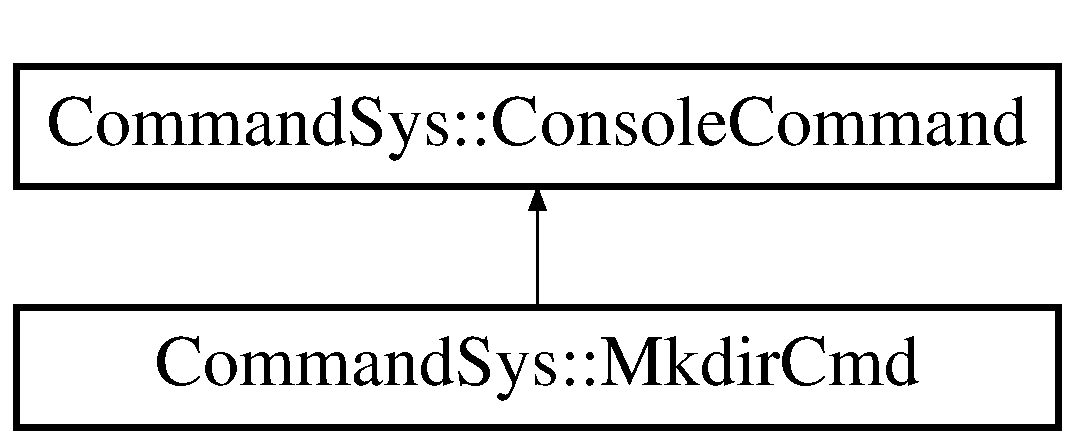
\includegraphics[height=2.000000cm]{class_command_sys_1_1_mkdir_cmd}
\end{center}
\end{figure}
\subsection*{Public 成员函数}
\begin{DoxyCompactItemize}
\item 
virtual void \hyperlink{class_command_sys_1_1_mkdir_cmd_a6a4c23d4e458c2ab12ca9da07625c1e1}{Execute} (void)
\begin{DoxyCompactList}\small\item\em 执行命令 \end{DoxyCompactList}\item 
\hypertarget{class_command_sys_1_1_mkdir_cmd_a7a578419fda8eb5d0a1042ac02ab9213}{virtual void {\bfseries Delete\-This} (void)}\label{class_command_sys_1_1_mkdir_cmd_a7a578419fda8eb5d0a1042ac02ab9213}

\end{DoxyCompactItemize}
\subsection*{额外继承的成员函数}


\subsection{详细描述}


在文件 Mkdir\-Cmd.\-h 第 9 行定义.



\subsection{成员函数说明}
\hypertarget{class_command_sys_1_1_mkdir_cmd_a6a4c23d4e458c2ab12ca9da07625c1e1}{\index{Command\-Sys\-::\-Mkdir\-Cmd@{Command\-Sys\-::\-Mkdir\-Cmd}!Execute@{Execute}}
\index{Execute@{Execute}!CommandSys::MkdirCmd@{Command\-Sys\-::\-Mkdir\-Cmd}}
\subsubsection[{Execute}]{\setlength{\rightskip}{0pt plus 5cm}void Command\-Sys\-::\-Mkdir\-Cmd\-::\-Execute (
\begin{DoxyParamCaption}
\item[{void}]{}
\end{DoxyParamCaption}
)\hspace{0.3cm}{\ttfamily [virtual]}}}\label{class_command_sys_1_1_mkdir_cmd_a6a4c23d4e458c2ab12ca9da07625c1e1}


执行命令 

\begin{DoxyRemark}{备注}
子类需重写该函数 
\end{DoxyRemark}


重载 \hyperlink{class_command_sys_1_1_console_command_a1d63e6780d3cfe83cc3452b0d797324c}{Command\-Sys\-::\-Console\-Command} .



在文件 Mkdir\-Cmd.\-cpp 第 19 行定义.



该类的文档由以下文件生成\-:\begin{DoxyCompactItemize}
\item 
Virtual\-Disk\-Console/Mkdir\-Cmd.\-h\item 
Virtual\-Disk\-Console/Mkdir\-Cmd.\-cpp\end{DoxyCompactItemize}

\hypertarget{class_file_sys_1_1_node}{\section{File\-Sys\-:\-:Node类 参考}
\label{class_file_sys_1_1_node}\index{File\-Sys\-::\-Node@{File\-Sys\-::\-Node}}
}
类 File\-Sys\-:\-:Node 继承关系图\-:\begin{figure}[H]
\begin{center}
\leavevmode
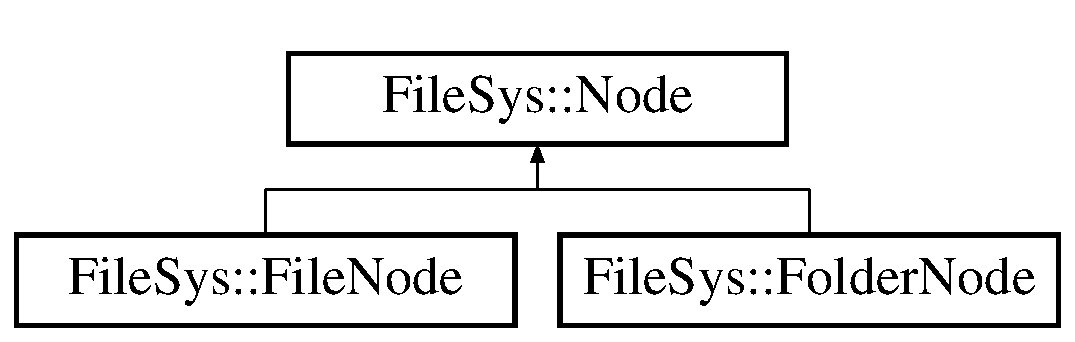
\includegraphics[height=2.000000cm]{class_file_sys_1_1_node}
\end{center}
\end{figure}
\subsection*{Public 类型}
\begin{DoxyCompactItemize}
\item 
enum {\bfseries Node\-Type} \{ {\bfseries F\-I\-L\-E\-\_\-\-N\-O\-D\-E} = 1, 
{\bfseries F\-O\-L\-D\-E\-R\-\_\-\-N\-O\-D\-E}
 \}
\end{DoxyCompactItemize}
\subsection*{Public 成员函数}
\begin{DoxyCompactItemize}
\item 
Util\-::\-String \hyperlink{class_file_sys_1_1_node_ac63b1d29e592028c77c70cbad8882834}{Name} () const 
\begin{DoxyCompactList}\small\item\em 返回节点名称 \end{DoxyCompactList}\item 
void \hyperlink{class_file_sys_1_1_node_a1d8a20f46e5036807ab404d04fc5da00}{Name} (const Util\-::\-String \&name)
\begin{DoxyCompactList}\small\item\em 设置节点名称 \end{DoxyCompactList}\item 
\hypertarget{class_file_sys_1_1_node_af1c666766a41b8acfeb7ddb447d22183}{Util\-::\-String \hyperlink{class_file_sys_1_1_node_af1c666766a41b8acfeb7ddb447d22183}{Path\-Name} (void) const }\label{class_file_sys_1_1_node_af1c666766a41b8acfeb7ddb447d22183}

\begin{DoxyCompactList}\small\item\em 获得当前节点的路径全名 \end{DoxyCompactList}\item 
\hyperlink{class_file_sys_1_1_node}{Node} $\ast$ \hyperlink{class_file_sys_1_1_node_a2de4a78fc6b8885d559f6d131f24cb8b}{Parent} (void) const 
\begin{DoxyCompactList}\small\item\em 返回父节点 \end{DoxyCompactList}\item 
void \hyperlink{class_file_sys_1_1_node_ae2519cd1f81789bb3e6ebb08a0da0916}{Parent} (\hyperlink{class_file_sys_1_1_node}{Node} $\ast$node)
\begin{DoxyCompactList}\small\item\em 设置父节点指针 \end{DoxyCompactList}\item 
bool \hyperlink{class_file_sys_1_1_node_a3a69d3f3c6021bb72057a490a799c4c6}{Is\-Leaf} (void) const 
\begin{DoxyCompactList}\small\item\em 是否为叶节点 \end{DoxyCompactList}\item 
bool \hyperlink{class_file_sys_1_1_node_afa19c01f76b54849fd4a95bc7e0ea7e2}{Is\-Root} (void) const 
\begin{DoxyCompactList}\small\item\em 是否为根节点 \end{DoxyCompactList}\item 
virtual bool \hyperlink{class_file_sys_1_1_node_abced0abf2d6f54f6b9887189c51c9bd1}{Is\-File} (void) const 
\begin{DoxyCompactList}\small\item\em 是否为文件 \end{DoxyCompactList}\item 
virtual bool \hyperlink{class_file_sys_1_1_node_ad93cc76a230827623b8fd1dbc255a9b2}{Is\-Folder} (void) const 
\begin{DoxyCompactList}\small\item\em 是否为文件夹 \end{DoxyCompactList}\item 
virtual bool \hyperlink{class_file_sys_1_1_node_a1c498398bb44692a5fe147e7466696bb}{Is\-Ancestor} (\hyperlink{class_file_sys_1_1_node}{Node} $\ast$node)
\begin{DoxyCompactList}\small\item\em 传入的节点是否为当前节点祖先 \end{DoxyCompactList}\item 
\hyperlink{class_file_sys_1_1_node}{Node} $\ast$ \hyperlink{class_file_sys_1_1_node_ab14d6ddc49b811ca57403992312a939a}{Find\-Node} (const Util\-::\-String \&name)
\begin{DoxyCompactList}\small\item\em 查找节点 \end{DoxyCompactList}\item 
\hyperlink{class_file_sys_1_1_node}{Node} $\ast$ \hyperlink{class_file_sys_1_1_node_ac55bdfd5962f88ac3c1848ad59dae30a}{Find\-File\-Node\-By\-Spec} (const Util\-::\-String \&spec)
\begin{DoxyCompactList}\small\item\em 查找该节点子节点是否有spec指定的文件后缀的节点 \end{DoxyCompactList}\item 
\hyperlink{class_file_sys_1_1_node}{Node} $\ast$ \hyperlink{class_file_sys_1_1_node_a442bb04445155587d095d628dbec6bf6}{Create\-Node} (const Util\-::\-String \&name, const Node\-Type type)
\begin{DoxyCompactList}\small\item\em 创建节点 \end{DoxyCompactList}\end{DoxyCompactItemize}
\subsection*{要删除的节点名称}
\label{_amgrpd279e7a5021fed3be0fd53799466000c}%
删除这名称指定的节点

\begin{DoxyReturn}{返回}
返回是否删除成功 
\end{DoxyReturn}

\begin{DoxyRetVals}{返回值}
{\em true} & 找到节点并删除成功 \\
\hline
{\em false} & 未找到节点 \\
\hline
\end{DoxyRetVals}
\begin{DoxyCompactItemize}
\item 
\hypertarget{class_file_sys_1_1_node_a982da8b0cc8f6f12d9b6fcea6890cade}{Util\-::\-String {\bfseries m\-\_\-name}}\label{class_file_sys_1_1_node_a982da8b0cc8f6f12d9b6fcea6890cade}

\item 
\hypertarget{class_file_sys_1_1_node_afef8b39b75789040417847af5efedbda}{\hyperlink{class_file_sys_1_1_node}{Node} $\ast$ \hyperlink{class_file_sys_1_1_node_afef8b39b75789040417847af5efedbda}{m\-\_\-lp\-\_\-parent}}\label{class_file_sys_1_1_node_afef8b39b75789040417847af5efedbda}

\begin{DoxyCompactList}\small\item\em $>$节点名称 \end{DoxyCompactList}\item 
\hypertarget{class_file_sys_1_1_node_a94704313dc4313ddde51129c73ec16c4}{\hyperlink{class_util_1_1_link_list_t}{Util\-::\-Link\-List\-T}$<$ \hyperlink{class_file_sys_1_1_node}{Node} $\ast$ $>$ \hyperlink{class_file_sys_1_1_node_a94704313dc4313ddde51129c73ec16c4}{m\-\_\-child\-\_\-nodes}}\label{class_file_sys_1_1_node_a94704313dc4313ddde51129c73ec16c4}

\begin{DoxyCompactList}\small\item\em $>$父节点指针 \end{DoxyCompactList}\item 
\hypertarget{class_file_sys_1_1_node_a4fcc133baeb1f8213fc5e886c40739da}{bool {\bfseries Delete\-Node} (const Util\-::\-String \&name)}\label{class_file_sys_1_1_node_a4fcc133baeb1f8213fc5e886c40739da}

\item 
\hypertarget{class_file_sys_1_1_node_a3366c9b2f3d63d629326eb65ef8ab6b2}{void \hyperlink{class_file_sys_1_1_node_a3366c9b2f3d63d629326eb65ef8ab6b2}{Delete\-Node\-By\-Type} (const Node\-Type type)}\label{class_file_sys_1_1_node_a3366c9b2f3d63d629326eb65ef8ab6b2}

\begin{DoxyCompactList}\small\item\em 删除该节点下属所指定类型的节点 \end{DoxyCompactList}\item 
\hypertarget{class_file_sys_1_1_node_ae6d82979ab6cc2fb80c04341cff5f88c}{virtual void \hyperlink{class_file_sys_1_1_node_ae6d82979ab6cc2fb80c04341cff5f88c}{Destroy} (void)}\label{class_file_sys_1_1_node_ae6d82979ab6cc2fb80c04341cff5f88c}

\begin{DoxyCompactList}\small\item\em 销毁结点自身信息 \end{DoxyCompactList}\item 
\hypertarget{class_file_sys_1_1_node_a1d20bc6ebbfe1642e061d39d1ed11142}{virtual void \hyperlink{class_file_sys_1_1_node_a1d20bc6ebbfe1642e061d39d1ed11142}{Delete\-This} (void)}\label{class_file_sys_1_1_node_a1d20bc6ebbfe1642e061d39d1ed11142}

\begin{DoxyCompactList}\small\item\em 删除自身 \end{DoxyCompactList}\item 
virtual void \hyperlink{class_file_sys_1_1_node_a6d56c256556bb453dbbce8885f7c7f6d}{Accept} (\hyperlink{class_file_sys_1_1_node_visitor}{Node\-Visitor} $\ast$visitor)
\begin{DoxyCompactList}\small\item\em 接手访问者访问 \end{DoxyCompactList}\item 
virtual int \hyperlink{class_file_sys_1_1_node_a3997a5d698f49b90ff3ecfdf53c55d21}{Copy} (const void $\ast$data, const D\-W\-O\-R\-D size)
\begin{DoxyCompactList}\small\item\em 将传入的数据拷贝给该文件 \end{DoxyCompactList}\item 
virtual int \hyperlink{class_file_sys_1_1_node_a230d3b6653f4365cce62746c2dd8aec8}{Read} (const D\-W\-O\-R\-D offset, const D\-W\-O\-R\-D size, void $\ast$data)
\begin{DoxyCompactList}\small\item\em 读取虚拟磁盘中文件数据 \end{DoxyCompactList}\item 
\hypertarget{class_file_sys_1_1_node_a29ba406d8ea68f1b7276ae6bbcc0b01a}{virtual void \hyperlink{class_file_sys_1_1_node_a29ba406d8ea68f1b7276ae6bbcc0b01a}{Clear\-Data} (void)}\label{class_file_sys_1_1_node_a29ba406d8ea68f1b7276ae6bbcc0b01a}

\begin{DoxyCompactList}\small\item\em 清空节点中附带的数据 \end{DoxyCompactList}\item 
virtual bool \hyperlink{class_file_sys_1_1_node_acad64b2ca2b78a0b634a49e6214c1aba}{Is\-Binary\-File} (void) const 
\begin{DoxyCompactList}\small\item\em 返回文件是否为二进制文件 \end{DoxyCompactList}\item 
virtual D\-W\-O\-R\-D \hyperlink{class_file_sys_1_1_node_a4d981a125be5d9e4810bf95f86dbd6bd}{Size} (void) const 
\begin{DoxyCompactList}\small\item\em 返回节点所含数据大小 \end{DoxyCompactList}\item 
virtual D\-W\-O\-R\-D \hyperlink{class_file_sys_1_1_node_a6f73b0fcebfed60297a7472a954be9eb}{Calc\-Total\-Size} (void)
\begin{DoxyCompactList}\small\item\em 递归计算该节点子树附带数据的总大小 \end{DoxyCompactList}\item 
virtual bool \hyperlink{class_file_sys_1_1_node_ada9acb89cd979b2e37d169d67e9ba816}{Compare} (const void $\ast$data, const D\-W\-O\-R\-D size, \hyperlink{class_util_1_1_vector_t}{Util\-::\-Vector\-T}$<$ char $>$ \&diff1, \hyperlink{class_util_1_1_vector_t}{Util\-::\-Vector\-T}$<$ char $>$ \&diff2) const 
\begin{DoxyCompactList}\small\item\em 比较指定缓冲区与当前文件的异同 \end{DoxyCompactList}\item 
virtual bool \hyperlink{class_file_sys_1_1_node_a61fe784ffa56a134715baa35a5a7e239}{Compare} (const H\-A\-N\-D\-L\-E file, \hyperlink{class_util_1_1_vector_t}{Util\-::\-Vector\-T}$<$ char $>$ \&diff1, \hyperlink{class_util_1_1_vector_t}{Util\-::\-Vector\-T}$<$ char $>$ \&diff2) const 
\begin{DoxyCompactList}\small\item\em 比较指定缓冲区与当前文件的异同 \end{DoxyCompactList}\item 
virtual void \hyperlink{class_file_sys_1_1_node_aea400658729cd06ba5c404ed67dd5abb}{Get\-File\-List\-Output\-String} (Util\-::\-String \&output, const bool recursive=false, const bool folder\-\_\-only=false) const 
\begin{DoxyCompactList}\small\item\em 获取文件列表打印字符串 \end{DoxyCompactList}\end{DoxyCompactItemize}


\subsection{详细描述}


在文件 Node.\-h 第 11 行定义.



\subsection{成员函数说明}
\hypertarget{class_file_sys_1_1_node_a6d56c256556bb453dbbce8885f7c7f6d}{\index{File\-Sys\-::\-Node@{File\-Sys\-::\-Node}!Accept@{Accept}}
\index{Accept@{Accept}!FileSys::Node@{File\-Sys\-::\-Node}}
\subsubsection[{Accept}]{\setlength{\rightskip}{0pt plus 5cm}void File\-Sys\-::\-Node\-::\-Accept (
\begin{DoxyParamCaption}
\item[{{\bf Node\-Visitor} $\ast$}]{visitor}
\end{DoxyParamCaption}
)\hspace{0.3cm}{\ttfamily [virtual]}}}\label{class_file_sys_1_1_node_a6d56c256556bb453dbbce8885f7c7f6d}


接手访问者访问 


\begin{DoxyParams}{参数}
{\em visitor} & 访问者 \\
\hline
\end{DoxyParams}


在文件 Node.\-cpp 第 208 行定义.

\hypertarget{class_file_sys_1_1_node_a6f73b0fcebfed60297a7472a954be9eb}{\index{File\-Sys\-::\-Node@{File\-Sys\-::\-Node}!Calc\-Total\-Size@{Calc\-Total\-Size}}
\index{Calc\-Total\-Size@{Calc\-Total\-Size}!FileSys::Node@{File\-Sys\-::\-Node}}
\subsubsection[{Calc\-Total\-Size}]{\setlength{\rightskip}{0pt plus 5cm}virtual D\-W\-O\-R\-D File\-Sys\-::\-Node\-::\-Calc\-Total\-Size (
\begin{DoxyParamCaption}
\item[{void}]{}
\end{DoxyParamCaption}
)\hspace{0.3cm}{\ttfamily [inline]}, {\ttfamily [virtual]}}}\label{class_file_sys_1_1_node_a6f73b0fcebfed60297a7472a954be9eb}


递归计算该节点子树附带数据的总大小 

\begin{DoxyReturn}{返回}
返回递归计算的子树附带数据大小 
\end{DoxyReturn}


被 \hyperlink{class_file_sys_1_1_file_node_acafc6eec61aafcf3e1899c9716ee3629}{File\-Sys\-::\-File\-Node} , 以及 \hyperlink{class_file_sys_1_1_folder_node_a6110e52309d675646c67b37e60b37ee5}{File\-Sys\-::\-Folder\-Node} 重载.



在文件 Node.\-h 第 177 行定义.

\hypertarget{class_file_sys_1_1_node_ada9acb89cd979b2e37d169d67e9ba816}{\index{File\-Sys\-::\-Node@{File\-Sys\-::\-Node}!Compare@{Compare}}
\index{Compare@{Compare}!FileSys::Node@{File\-Sys\-::\-Node}}
\subsubsection[{Compare}]{\setlength{\rightskip}{0pt plus 5cm}virtual bool File\-Sys\-::\-Node\-::\-Compare (
\begin{DoxyParamCaption}
\item[{const void $\ast$}]{data, }
\item[{const D\-W\-O\-R\-D}]{size, }
\item[{{\bf Util\-::\-Vector\-T}$<$ char $>$ \&}]{diff1, }
\item[{{\bf Util\-::\-Vector\-T}$<$ char $>$ \&}]{diff2}
\end{DoxyParamCaption}
) const\hspace{0.3cm}{\ttfamily [inline]}, {\ttfamily [virtual]}}}\label{class_file_sys_1_1_node_ada9acb89cd979b2e37d169d67e9ba816}


比较指定缓冲区与当前文件的异同 


\begin{DoxyParams}{参数}
{\em data} & 待比较的缓冲区 \\
\hline
{\em size} & 缓冲区中数据的大小 \\
\hline
{\em diff1} & 返回的本文件从第一个不同字节起始处往后的16个字节数组 \\
\hline
{\em diff2} & 返回的磁盘文件从第一个不同字节起始处往后的16个字节数组 \\
\hline
\end{DoxyParams}
\begin{DoxyReturn}{返回}
返回比较是否相同 
\end{DoxyReturn}

\begin{DoxyRetVals}{返回值}
{\em true} & 比较结果相同 \\
\hline
{\em false} & 比较结果不同 \\
\hline
\end{DoxyRetVals}
\begin{DoxyRemark}{备注}
若data为\-N\-U\-L\-L或size为0的情况下也会返回false 
\end{DoxyRemark}


被 \hyperlink{class_file_sys_1_1_file_node_afd998a6e6747f426c856ccdedd21eeb6}{File\-Sys\-::\-File\-Node} 重载.



在文件 Node.\-h 第 190 行定义.

\hypertarget{class_file_sys_1_1_node_a61fe784ffa56a134715baa35a5a7e239}{\index{File\-Sys\-::\-Node@{File\-Sys\-::\-Node}!Compare@{Compare}}
\index{Compare@{Compare}!FileSys::Node@{File\-Sys\-::\-Node}}
\subsubsection[{Compare}]{\setlength{\rightskip}{0pt plus 5cm}virtual bool File\-Sys\-::\-Node\-::\-Compare (
\begin{DoxyParamCaption}
\item[{const H\-A\-N\-D\-L\-E}]{file, }
\item[{{\bf Util\-::\-Vector\-T}$<$ char $>$ \&}]{diff1, }
\item[{{\bf Util\-::\-Vector\-T}$<$ char $>$ \&}]{diff2}
\end{DoxyParamCaption}
) const\hspace{0.3cm}{\ttfamily [inline]}, {\ttfamily [virtual]}}}\label{class_file_sys_1_1_node_a61fe784ffa56a134715baa35a5a7e239}


比较指定缓冲区与当前文件的异同 


\begin{DoxyParams}{参数}
{\em file} & 待比较的磁盘文件句柄 \\
\hline
{\em diff1} & 返回的本文件从第一个不同字节起始处往后的16个字节数组 \\
\hline
{\em diff2} & 返回的磁盘文件从第一个不同字节起始处往后的16个字节数组 \\
\hline
\end{DoxyParams}
\begin{DoxyReturn}{返回}
返回比较是否相同 
\end{DoxyReturn}

\begin{DoxyRetVals}{返回值}
{\em true} & 比较结果相同 \\
\hline
{\em false} & 比较结果不同 \\
\hline
\end{DoxyRetVals}
\begin{DoxyRemark}{备注}
若data为\-N\-U\-L\-L或size为0的情况下也会返回false 
\end{DoxyRemark}


被 \hyperlink{class_file_sys_1_1_file_node_aa14e75686fe236425f4580763bd75222}{File\-Sys\-::\-File\-Node} 重载.



在文件 Node.\-h 第 202 行定义.

\hypertarget{class_file_sys_1_1_node_a3997a5d698f49b90ff3ecfdf53c55d21}{\index{File\-Sys\-::\-Node@{File\-Sys\-::\-Node}!Copy@{Copy}}
\index{Copy@{Copy}!FileSys::Node@{File\-Sys\-::\-Node}}
\subsubsection[{Copy}]{\setlength{\rightskip}{0pt plus 5cm}virtual int File\-Sys\-::\-Node\-::\-Copy (
\begin{DoxyParamCaption}
\item[{const void $\ast$}]{data, }
\item[{const D\-W\-O\-R\-D}]{size}
\end{DoxyParamCaption}
)\hspace{0.3cm}{\ttfamily [inline]}, {\ttfamily [virtual]}}}\label{class_file_sys_1_1_node_a3997a5d698f49b90ff3ecfdf53c55d21}


将传入的数据拷贝给该文件 


\begin{DoxyParams}{参数}
{\em data} & 欲拷贝的数据缓冲区指针,此缓冲区由该文件节点负责释放内存 \\
\hline
{\em size} & 数据缓冲区中数据大小 \\
\hline
\end{DoxyParams}
\begin{DoxyReturn}{返回}
返回实际拷贝的数据大小 
\end{DoxyReturn}


被 \hyperlink{class_file_sys_1_1_file_node_a4284926acb04ef0ab0db8b73d2f1fba1}{File\-Sys\-::\-File\-Node} 重载.



在文件 Node.\-h 第 143 行定义.

\hypertarget{class_file_sys_1_1_node_a442bb04445155587d095d628dbec6bf6}{\index{File\-Sys\-::\-Node@{File\-Sys\-::\-Node}!Create\-Node@{Create\-Node}}
\index{Create\-Node@{Create\-Node}!FileSys::Node@{File\-Sys\-::\-Node}}
\subsubsection[{Create\-Node}]{\setlength{\rightskip}{0pt plus 5cm}{\bf Node} $\ast$ File\-Sys\-::\-Node\-::\-Create\-Node (
\begin{DoxyParamCaption}
\item[{const Util\-::\-String \&}]{name, }
\item[{const Node\-Type}]{type}
\end{DoxyParamCaption}
)}}\label{class_file_sys_1_1_node_a442bb04445155587d095d628dbec6bf6}


创建节点 


\begin{DoxyParams}{参数}
{\em name} & 节点名称 \\
\hline
{\em type} & 节点类型 \\
\hline
\end{DoxyParams}
\begin{DoxyReturn}{返回}
返回创建的节点 
\end{DoxyReturn}


在文件 Node.\-cpp 第 96 行定义.

\hypertarget{class_file_sys_1_1_node_ac55bdfd5962f88ac3c1848ad59dae30a}{\index{File\-Sys\-::\-Node@{File\-Sys\-::\-Node}!Find\-File\-Node\-By\-Spec@{Find\-File\-Node\-By\-Spec}}
\index{Find\-File\-Node\-By\-Spec@{Find\-File\-Node\-By\-Spec}!FileSys::Node@{File\-Sys\-::\-Node}}
\subsubsection[{Find\-File\-Node\-By\-Spec}]{\setlength{\rightskip}{0pt plus 5cm}{\bf Node} $\ast$ File\-Sys\-::\-Node\-::\-Find\-File\-Node\-By\-Spec (
\begin{DoxyParamCaption}
\item[{const Util\-::\-String \&}]{spec}
\end{DoxyParamCaption}
)}}\label{class_file_sys_1_1_node_ac55bdfd5962f88ac3c1848ad59dae30a}


查找该节点子节点是否有spec指定的文件后缀的节点 

\begin{DoxyReturn}{返回}
查找到的文件节点 
\end{DoxyReturn}

\begin{DoxyRetVals}{返回值}
{\em N\-U\-L\-L} & 查找失败 \\
\hline
\end{DoxyRetVals}


在文件 Node.\-cpp 第 53 行定义.

\hypertarget{class_file_sys_1_1_node_ab14d6ddc49b811ca57403992312a939a}{\index{File\-Sys\-::\-Node@{File\-Sys\-::\-Node}!Find\-Node@{Find\-Node}}
\index{Find\-Node@{Find\-Node}!FileSys::Node@{File\-Sys\-::\-Node}}
\subsubsection[{Find\-Node}]{\setlength{\rightskip}{0pt plus 5cm}{\bf Node} $\ast$ File\-Sys\-::\-Node\-::\-Find\-Node (
\begin{DoxyParamCaption}
\item[{const Util\-::\-String \&}]{name}
\end{DoxyParamCaption}
)}}\label{class_file_sys_1_1_node_ab14d6ddc49b811ca57403992312a939a}


查找节点 


\begin{DoxyParams}{参数}
{\em name} & 要查找名称 \\
\hline
\end{DoxyParams}
\begin{DoxyReturn}{返回}
查找的节点 
\end{DoxyReturn}


在文件 Node.\-cpp 第 34 行定义.

\hypertarget{class_file_sys_1_1_node_aea400658729cd06ba5c404ed67dd5abb}{\index{File\-Sys\-::\-Node@{File\-Sys\-::\-Node}!Get\-File\-List\-Output\-String@{Get\-File\-List\-Output\-String}}
\index{Get\-File\-List\-Output\-String@{Get\-File\-List\-Output\-String}!FileSys::Node@{File\-Sys\-::\-Node}}
\subsubsection[{Get\-File\-List\-Output\-String}]{\setlength{\rightskip}{0pt plus 5cm}void File\-Sys\-::\-Node\-::\-Get\-File\-List\-Output\-String (
\begin{DoxyParamCaption}
\item[{Util\-::\-String \&}]{output, }
\item[{const bool}]{recursive = {\ttfamily false}, }
\item[{const bool}]{folder\-\_\-only = {\ttfamily false}}
\end{DoxyParamCaption}
) const\hspace{0.3cm}{\ttfamily [virtual]}}}\label{class_file_sys_1_1_node_aea400658729cd06ba5c404ed67dd5abb}


获取文件列表打印字符串 


\begin{DoxyParams}{参数}
{\em output} & 为最终存放文件列表的字符串 \\
\hline
{\em recursive} & 指示是否是递归显示子目录与子文件 \\
\hline
\end{DoxyParams}


被 \hyperlink{class_file_sys_1_1_folder_node_a49bedb5a2504bdc13a86bcd38aa31ef6}{File\-Sys\-::\-Folder\-Node} 重载.



在文件 Node.\-cpp 第 214 行定义.

\hypertarget{class_file_sys_1_1_node_a1c498398bb44692a5fe147e7466696bb}{\index{File\-Sys\-::\-Node@{File\-Sys\-::\-Node}!Is\-Ancestor@{Is\-Ancestor}}
\index{Is\-Ancestor@{Is\-Ancestor}!FileSys::Node@{File\-Sys\-::\-Node}}
\subsubsection[{Is\-Ancestor}]{\setlength{\rightskip}{0pt plus 5cm}bool File\-Sys\-::\-Node\-::\-Is\-Ancestor (
\begin{DoxyParamCaption}
\item[{{\bf Node} $\ast$}]{node}
\end{DoxyParamCaption}
)\hspace{0.3cm}{\ttfamily [virtual]}}}\label{class_file_sys_1_1_node_a1c498398bb44692a5fe147e7466696bb}


传入的节点是否为当前节点祖先 

\begin{DoxyReturn}{返回}
返回是否为祖先 
\end{DoxyReturn}

\begin{DoxyRetVals}{返回值}
{\em true} & 是祖先节点 \\
\hline
{\em false} & 不是祖先节点 \\
\hline
\end{DoxyRetVals}


在文件 Node.\-cpp 第 77 行定义.

\hypertarget{class_file_sys_1_1_node_acad64b2ca2b78a0b634a49e6214c1aba}{\index{File\-Sys\-::\-Node@{File\-Sys\-::\-Node}!Is\-Binary\-File@{Is\-Binary\-File}}
\index{Is\-Binary\-File@{Is\-Binary\-File}!FileSys::Node@{File\-Sys\-::\-Node}}
\subsubsection[{Is\-Binary\-File}]{\setlength{\rightskip}{0pt plus 5cm}virtual bool File\-Sys\-::\-Node\-::\-Is\-Binary\-File (
\begin{DoxyParamCaption}
\item[{void}]{}
\end{DoxyParamCaption}
) const\hspace{0.3cm}{\ttfamily [inline]}, {\ttfamily [virtual]}}}\label{class_file_sys_1_1_node_acad64b2ca2b78a0b634a49e6214c1aba}


返回文件是否为二进制文件 

\begin{DoxyReturn}{返回}
返回文件是否是二进制文件 
\end{DoxyReturn}

\begin{DoxyRetVals}{返回值}
{\em true} & 为二进制文件 \\
\hline
{\em false} & 为文本文件 \\
\hline
\end{DoxyRetVals}


被 \hyperlink{class_file_sys_1_1_file_node_a0bf53af4d6c34922bc1c667415b65d5c}{File\-Sys\-::\-File\-Node} 重载.



在文件 Node.\-h 第 165 行定义.

\hypertarget{class_file_sys_1_1_node_abced0abf2d6f54f6b9887189c51c9bd1}{\index{File\-Sys\-::\-Node@{File\-Sys\-::\-Node}!Is\-File@{Is\-File}}
\index{Is\-File@{Is\-File}!FileSys::Node@{File\-Sys\-::\-Node}}
\subsubsection[{Is\-File}]{\setlength{\rightskip}{0pt plus 5cm}virtual bool File\-Sys\-::\-Node\-::\-Is\-File (
\begin{DoxyParamCaption}
\item[{void}]{}
\end{DoxyParamCaption}
) const\hspace{0.3cm}{\ttfamily [inline]}, {\ttfamily [virtual]}}}\label{class_file_sys_1_1_node_abced0abf2d6f54f6b9887189c51c9bd1}


是否为文件 

\begin{DoxyReturn}{返回}
返回是否为文件 
\end{DoxyReturn}


被 \hyperlink{class_file_sys_1_1_file_node_a8a9c01da1c043554743877aff68ddad9}{File\-Sys\-::\-File\-Node} 重载.



在文件 Node.\-h 第 68 行定义.

\hypertarget{class_file_sys_1_1_node_ad93cc76a230827623b8fd1dbc255a9b2}{\index{File\-Sys\-::\-Node@{File\-Sys\-::\-Node}!Is\-Folder@{Is\-Folder}}
\index{Is\-Folder@{Is\-Folder}!FileSys::Node@{File\-Sys\-::\-Node}}
\subsubsection[{Is\-Folder}]{\setlength{\rightskip}{0pt plus 5cm}virtual bool File\-Sys\-::\-Node\-::\-Is\-Folder (
\begin{DoxyParamCaption}
\item[{void}]{}
\end{DoxyParamCaption}
) const\hspace{0.3cm}{\ttfamily [inline]}, {\ttfamily [virtual]}}}\label{class_file_sys_1_1_node_ad93cc76a230827623b8fd1dbc255a9b2}


是否为文件夹 

\begin{DoxyReturn}{返回}
返回是否为文件夹 
\end{DoxyReturn}


被 \hyperlink{class_file_sys_1_1_folder_node_a050961bdc9d98b7645bc518e215dd929}{File\-Sys\-::\-Folder\-Node} 重载.



在文件 Node.\-h 第 74 行定义.

\hypertarget{class_file_sys_1_1_node_a3a69d3f3c6021bb72057a490a799c4c6}{\index{File\-Sys\-::\-Node@{File\-Sys\-::\-Node}!Is\-Leaf@{Is\-Leaf}}
\index{Is\-Leaf@{Is\-Leaf}!FileSys::Node@{File\-Sys\-::\-Node}}
\subsubsection[{Is\-Leaf}]{\setlength{\rightskip}{0pt plus 5cm}bool File\-Sys\-::\-Node\-::\-Is\-Leaf (
\begin{DoxyParamCaption}
\item[{void}]{}
\end{DoxyParamCaption}
) const\hspace{0.3cm}{\ttfamily [inline]}}}\label{class_file_sys_1_1_node_a3a69d3f3c6021bb72057a490a799c4c6}


是否为叶节点 

\begin{DoxyReturn}{返回}
返回节点是否为叶节点 
\end{DoxyReturn}


在文件 Node.\-h 第 56 行定义.

\hypertarget{class_file_sys_1_1_node_afa19c01f76b54849fd4a95bc7e0ea7e2}{\index{File\-Sys\-::\-Node@{File\-Sys\-::\-Node}!Is\-Root@{Is\-Root}}
\index{Is\-Root@{Is\-Root}!FileSys::Node@{File\-Sys\-::\-Node}}
\subsubsection[{Is\-Root}]{\setlength{\rightskip}{0pt plus 5cm}bool File\-Sys\-::\-Node\-::\-Is\-Root (
\begin{DoxyParamCaption}
\item[{void}]{}
\end{DoxyParamCaption}
) const\hspace{0.3cm}{\ttfamily [inline]}}}\label{class_file_sys_1_1_node_afa19c01f76b54849fd4a95bc7e0ea7e2}


是否为根节点 

\begin{DoxyReturn}{返回}
返回节点是否为根节点 
\end{DoxyReturn}


在文件 Node.\-h 第 62 行定义.

\hypertarget{class_file_sys_1_1_node_ac63b1d29e592028c77c70cbad8882834}{\index{File\-Sys\-::\-Node@{File\-Sys\-::\-Node}!Name@{Name}}
\index{Name@{Name}!FileSys::Node@{File\-Sys\-::\-Node}}
\subsubsection[{Name}]{\setlength{\rightskip}{0pt plus 5cm}Util\-::\-String File\-Sys\-::\-Node\-::\-Name (
\begin{DoxyParamCaption}
{}
\end{DoxyParamCaption}
) const\hspace{0.3cm}{\ttfamily [inline]}}}\label{class_file_sys_1_1_node_ac63b1d29e592028c77c70cbad8882834}


返回节点名称 

\begin{DoxyReturn}{返回}
返回名称 
\end{DoxyReturn}


在文件 Node.\-h 第 27 行定义.

\hypertarget{class_file_sys_1_1_node_a1d8a20f46e5036807ab404d04fc5da00}{\index{File\-Sys\-::\-Node@{File\-Sys\-::\-Node}!Name@{Name}}
\index{Name@{Name}!FileSys::Node@{File\-Sys\-::\-Node}}
\subsubsection[{Name}]{\setlength{\rightskip}{0pt plus 5cm}void File\-Sys\-::\-Node\-::\-Name (
\begin{DoxyParamCaption}
\item[{const Util\-::\-String \&}]{name}
\end{DoxyParamCaption}
)\hspace{0.3cm}{\ttfamily [inline]}}}\label{class_file_sys_1_1_node_a1d8a20f46e5036807ab404d04fc5da00}


设置节点名称 


\begin{DoxyParams}{参数}
{\em name} & 节点名称 \\
\hline
\end{DoxyParams}


在文件 Node.\-h 第 33 行定义.

\hypertarget{class_file_sys_1_1_node_a2de4a78fc6b8885d559f6d131f24cb8b}{\index{File\-Sys\-::\-Node@{File\-Sys\-::\-Node}!Parent@{Parent}}
\index{Parent@{Parent}!FileSys::Node@{File\-Sys\-::\-Node}}
\subsubsection[{Parent}]{\setlength{\rightskip}{0pt plus 5cm}{\bf Node}$\ast$ File\-Sys\-::\-Node\-::\-Parent (
\begin{DoxyParamCaption}
\item[{void}]{}
\end{DoxyParamCaption}
) const\hspace{0.3cm}{\ttfamily [inline]}}}\label{class_file_sys_1_1_node_a2de4a78fc6b8885d559f6d131f24cb8b}


返回父节点 

\begin{DoxyReturn}{返回}
父节点指针 
\end{DoxyReturn}


在文件 Node.\-h 第 44 行定义.

\hypertarget{class_file_sys_1_1_node_ae2519cd1f81789bb3e6ebb08a0da0916}{\index{File\-Sys\-::\-Node@{File\-Sys\-::\-Node}!Parent@{Parent}}
\index{Parent@{Parent}!FileSys::Node@{File\-Sys\-::\-Node}}
\subsubsection[{Parent}]{\setlength{\rightskip}{0pt plus 5cm}void File\-Sys\-::\-Node\-::\-Parent (
\begin{DoxyParamCaption}
\item[{{\bf Node} $\ast$}]{node}
\end{DoxyParamCaption}
)\hspace{0.3cm}{\ttfamily [inline]}}}\label{class_file_sys_1_1_node_ae2519cd1f81789bb3e6ebb08a0da0916}


设置父节点指针 


\begin{DoxyParams}{参数}
{\em node} & 父节点指针 \\
\hline
\end{DoxyParams}


在文件 Node.\-h 第 50 行定义.

\hypertarget{class_file_sys_1_1_node_a230d3b6653f4365cce62746c2dd8aec8}{\index{File\-Sys\-::\-Node@{File\-Sys\-::\-Node}!Read@{Read}}
\index{Read@{Read}!FileSys::Node@{File\-Sys\-::\-Node}}
\subsubsection[{Read}]{\setlength{\rightskip}{0pt plus 5cm}virtual int File\-Sys\-::\-Node\-::\-Read (
\begin{DoxyParamCaption}
\item[{const D\-W\-O\-R\-D}]{offset, }
\item[{const D\-W\-O\-R\-D}]{size, }
\item[{void $\ast$}]{data}
\end{DoxyParamCaption}
)\hspace{0.3cm}{\ttfamily [inline]}, {\ttfamily [virtual]}}}\label{class_file_sys_1_1_node_a230d3b6653f4365cce62746c2dd8aec8}


读取虚拟磁盘中文件数据 


\begin{DoxyParams}{参数}
{\em offset} & 读取偏移值(按字节计) \\
\hline
{\em size} & 要读取数据的大小 \\
\hline
{\em data} & 读取数据存入的数据缓冲区指针 \\
\hline
\end{DoxyParams}
\begin{DoxyReturn}{返回}
实际读取的数据大小 
\end{DoxyReturn}


被 \hyperlink{class_file_sys_1_1_file_node_a63de509985ada5a7cedfc46c1e4e1277}{File\-Sys\-::\-File\-Node} 重载.



在文件 Node.\-h 第 152 行定义.

\hypertarget{class_file_sys_1_1_node_a4d981a125be5d9e4810bf95f86dbd6bd}{\index{File\-Sys\-::\-Node@{File\-Sys\-::\-Node}!Size@{Size}}
\index{Size@{Size}!FileSys::Node@{File\-Sys\-::\-Node}}
\subsubsection[{Size}]{\setlength{\rightskip}{0pt plus 5cm}virtual D\-W\-O\-R\-D File\-Sys\-::\-Node\-::\-Size (
\begin{DoxyParamCaption}
\item[{void}]{}
\end{DoxyParamCaption}
) const\hspace{0.3cm}{\ttfamily [inline]}, {\ttfamily [virtual]}}}\label{class_file_sys_1_1_node_a4d981a125be5d9e4810bf95f86dbd6bd}


返回节点所含数据大小 

\begin{DoxyReturn}{返回}
节点所含的数据大小按字节计 
\end{DoxyReturn}


被 \hyperlink{class_file_sys_1_1_file_node_ac66c3549ac94e6ca8e5adde3970f6421}{File\-Sys\-::\-File\-Node} 重载.



在文件 Node.\-h 第 171 行定义.



该类的文档由以下文件生成\-:\begin{DoxyCompactItemize}
\item 
Virtual\-Disk\-Console/Node.\-h\item 
Virtual\-Disk\-Console/Node.\-cpp\end{DoxyCompactItemize}

\hypertarget{class_file_sys_1_1_node_visitor}{\section{File\-Sys\-:\-:Node\-Visitor类 参考}
\label{class_file_sys_1_1_node_visitor}\index{File\-Sys\-::\-Node\-Visitor@{File\-Sys\-::\-Node\-Visitor}}
}
类 File\-Sys\-:\-:Node\-Visitor 继承关系图\-:\begin{figure}[H]
\begin{center}
\leavevmode
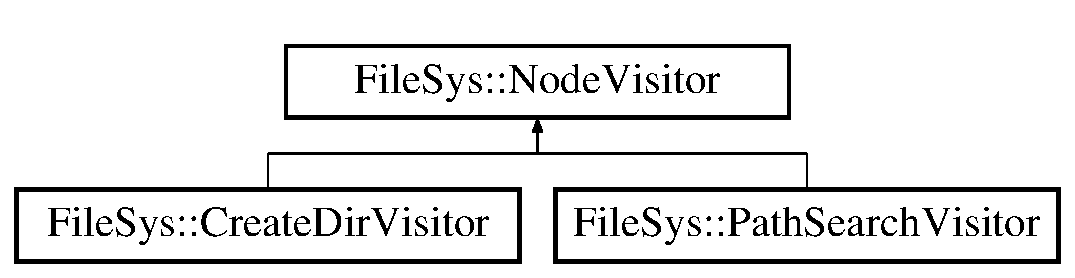
\includegraphics[height=2.000000cm]{class_file_sys_1_1_node_visitor}
\end{center}
\end{figure}
\subsection*{Public 成员函数}
\begin{DoxyCompactItemize}
\item 
virtual void \hyperlink{class_file_sys_1_1_node_visitor_ac493ab442e116be15f0af8559d63e0e0}{Set\-Path} (const \hyperlink{class_lexer_sys_1_1_search_path}{Lexer\-Sys\-::\-Search\-Path} \&path)
\begin{DoxyCompactList}\small\item\em 设置搜索路径 \end{DoxyCompactList}\item 
virtual \hyperlink{class_lexer_sys_1_1_token}{Lexer\-Sys\-::\-Token} \hyperlink{class_file_sys_1_1_node_visitor_a2cfda47a2803438cb97b0e8b83dbdb79}{Get\-Curr\-Path\-Token} (void) const 
\begin{DoxyCompactList}\small\item\em 获得搜索路径的当前符号 \end{DoxyCompactList}\item 
\hypertarget{class_file_sys_1_1_node_visitor_add992fdbc0bad4e4bdc25025ce8e8a58}{virtual bool \hyperlink{class_file_sys_1_1_node_visitor_add992fdbc0bad4e4bdc25025ce8e8a58}{Has\-Next\-Token} (void) const }\label{class_file_sys_1_1_node_visitor_add992fdbc0bad4e4bdc25025ce8e8a58}

\begin{DoxyCompactList}\small\item\em 是否还有下一个符号 \end{DoxyCompactList}\item 
\hypertarget{class_file_sys_1_1_node_visitor_a2438bc4ed66436f340f02357461c2836}{virtual void \hyperlink{class_file_sys_1_1_node_visitor_a2438bc4ed66436f340f02357461c2836}{Move\-To\-Next\-Token} (void)}\label{class_file_sys_1_1_node_visitor_a2438bc4ed66436f340f02357461c2836}

\begin{DoxyCompactList}\small\item\em 移动到搜索路径的下一个符号 \end{DoxyCompactList}\item 
\hypertarget{class_file_sys_1_1_node_visitor_acb8de479df2e49b6b68ebe2aa1727d71}{virtual \hyperlink{class_file_sys_1_1_node}{Node} $\ast$ \hyperlink{class_file_sys_1_1_node_visitor_acb8de479df2e49b6b68ebe2aa1727d71}{Get\-Search\-Node} (void)}\label{class_file_sys_1_1_node_visitor_acb8de479df2e49b6b68ebe2aa1727d71}

\begin{DoxyCompactList}\small\item\em 获得搜索到的节点 \end{DoxyCompactList}\item 
\hypertarget{class_file_sys_1_1_node_visitor_a75c0566ce6177629732cc0fc8d500c59}{virtual Util\-::\-String \hyperlink{class_file_sys_1_1_node_visitor_a75c0566ce6177629732cc0fc8d500c59}{Get\-Result\-Output\-String} (void) const }\label{class_file_sys_1_1_node_visitor_a75c0566ce6177629732cc0fc8d500c59}

\begin{DoxyCompactList}\small\item\em 获得搜索结果的输出字符串 \end{DoxyCompactList}\item 
virtual void \hyperlink{class_file_sys_1_1_node_visitor_a3398560bc10e71a0b8fcaac57e5b58e2}{Visit} (\hyperlink{class_file_sys_1_1_node}{Node} $\ast$node)
\begin{DoxyCompactList}\small\item\em 访问节点 \end{DoxyCompactList}\end{DoxyCompactItemize}
\subsection*{Protected 类型}
\begin{DoxyCompactItemize}
\item 
\hypertarget{class_file_sys_1_1_node_visitor_aa0480a8d4c26e612bb11e8f1c7da929e}{typedef \hyperlink{class_util_1_1_link_list_t}{Util\-::\-Link\-List\-T}\\*
$<$ \hyperlink{class_lexer_sys_1_1_token}{Lexer\-Sys\-::\-Token} $>$ {\bfseries Path\-Toks}}\label{class_file_sys_1_1_node_visitor_aa0480a8d4c26e612bb11e8f1c7da929e}

\end{DoxyCompactItemize}
\subsection*{Protected 属性}
\begin{DoxyCompactItemize}
\item 
\hypertarget{class_file_sys_1_1_node_visitor_a9985967f38e74d6e291330e7d609d21d}{\hyperlink{class_lexer_sys_1_1_search_path}{Lexer\-Sys\-::\-Search\-Path} {\bfseries m\-\_\-path}}\label{class_file_sys_1_1_node_visitor_a9985967f38e74d6e291330e7d609d21d}

\item 
\hypertarget{class_file_sys_1_1_node_visitor_adec163e2daf9387ddef7166162820881}{\hyperlink{class_file_sys_1_1_node}{Node} $\ast$ \hyperlink{class_file_sys_1_1_node_visitor_adec163e2daf9387ddef7166162820881}{m\-\_\-lp\-\_\-final\-\_\-search\-\_\-node}}\label{class_file_sys_1_1_node_visitor_adec163e2daf9387ddef7166162820881}

\begin{DoxyCompactList}\small\item\em $>$搜索路径 \end{DoxyCompactList}\item 
\hypertarget{class_file_sys_1_1_node_visitor_ad2f5269bc83504009525d7fde95e99bf}{Util\-::\-String \hyperlink{class_file_sys_1_1_node_visitor_ad2f5269bc83504009525d7fde95e99bf}{m\-\_\-result\-\_\-output\-\_\-str}}\label{class_file_sys_1_1_node_visitor_ad2f5269bc83504009525d7fde95e99bf}

\begin{DoxyCompactList}\small\item\em $>$当前节点 \end{DoxyCompactList}\end{DoxyCompactItemize}


\subsection{详细描述}


在文件 Node\-Visitor.\-h 第 12 行定义.



\subsection{成员函数说明}
\hypertarget{class_file_sys_1_1_node_visitor_a2cfda47a2803438cb97b0e8b83dbdb79}{\index{File\-Sys\-::\-Node\-Visitor@{File\-Sys\-::\-Node\-Visitor}!Get\-Curr\-Path\-Token@{Get\-Curr\-Path\-Token}}
\index{Get\-Curr\-Path\-Token@{Get\-Curr\-Path\-Token}!FileSys::NodeVisitor@{File\-Sys\-::\-Node\-Visitor}}
\subsubsection[{Get\-Curr\-Path\-Token}]{\setlength{\rightskip}{0pt plus 5cm}{\bf Lexer\-Sys\-::\-Token} File\-Sys\-::\-Node\-Visitor\-::\-Get\-Curr\-Path\-Token (
\begin{DoxyParamCaption}
\item[{void}]{}
\end{DoxyParamCaption}
) const\hspace{0.3cm}{\ttfamily [virtual]}}}\label{class_file_sys_1_1_node_visitor_a2cfda47a2803438cb97b0e8b83dbdb79}


获得搜索路径的当前符号 

\begin{DoxyReturn}{返回}
搜索路径的当前符号 
\end{DoxyReturn}


在文件 Node\-Visitor.\-cpp 第 22 行定义.

\hypertarget{class_file_sys_1_1_node_visitor_ac493ab442e116be15f0af8559d63e0e0}{\index{File\-Sys\-::\-Node\-Visitor@{File\-Sys\-::\-Node\-Visitor}!Set\-Path@{Set\-Path}}
\index{Set\-Path@{Set\-Path}!FileSys::NodeVisitor@{File\-Sys\-::\-Node\-Visitor}}
\subsubsection[{Set\-Path}]{\setlength{\rightskip}{0pt plus 5cm}void File\-Sys\-::\-Node\-Visitor\-::\-Set\-Path (
\begin{DoxyParamCaption}
\item[{const {\bf Lexer\-Sys\-::\-Search\-Path} \&}]{path}
\end{DoxyParamCaption}
)\hspace{0.3cm}{\ttfamily [virtual]}}}\label{class_file_sys_1_1_node_visitor_ac493ab442e116be15f0af8559d63e0e0}


设置搜索路径 


\begin{DoxyParams}{参数}
{\em path} & 搜索路径 \\
\hline
\end{DoxyParams}


在文件 Node\-Visitor.\-cpp 第 17 行定义.

\hypertarget{class_file_sys_1_1_node_visitor_a3398560bc10e71a0b8fcaac57e5b58e2}{\index{File\-Sys\-::\-Node\-Visitor@{File\-Sys\-::\-Node\-Visitor}!Visit@{Visit}}
\index{Visit@{Visit}!FileSys::NodeVisitor@{File\-Sys\-::\-Node\-Visitor}}
\subsubsection[{Visit}]{\setlength{\rightskip}{0pt plus 5cm}virtual void File\-Sys\-::\-Node\-Visitor\-::\-Visit (
\begin{DoxyParamCaption}
\item[{{\bf Node} $\ast$}]{node}
\end{DoxyParamCaption}
)\hspace{0.3cm}{\ttfamily [inline]}, {\ttfamily [virtual]}}}\label{class_file_sys_1_1_node_visitor_a3398560bc10e71a0b8fcaac57e5b58e2}


访问节点 


\begin{DoxyParams}{参数}
{\em node} & 待访问节点 \\
\hline
\end{DoxyParams}


被 \hyperlink{class_file_sys_1_1_path_search_visitor_ac9e8ab4c8389b118ba6a57b053ac8005}{File\-Sys\-::\-Path\-Search\-Visitor} , 以及 \hyperlink{class_file_sys_1_1_create_dir_visitor_a02c79d46c769edbbcff38a59a97811ab}{File\-Sys\-::\-Create\-Dir\-Visitor} 重载.



在文件 Node\-Visitor.\-h 第 55 行定义.



该类的文档由以下文件生成\-:\begin{DoxyCompactItemize}
\item 
Virtual\-Disk\-Console/Node\-Visitor.\-h\item 
Virtual\-Disk\-Console/Node\-Visitor.\-cpp\end{DoxyCompactItemize}

\hypertarget{class_file_sys_1_1_path_search_visitor}{\section{File\-Sys\-:\-:Path\-Search\-Visitor类 参考}
\label{class_file_sys_1_1_path_search_visitor}\index{File\-Sys\-::\-Path\-Search\-Visitor@{File\-Sys\-::\-Path\-Search\-Visitor}}
}
类 File\-Sys\-:\-:Path\-Search\-Visitor 继承关系图\-:\begin{figure}[H]
\begin{center}
\leavevmode
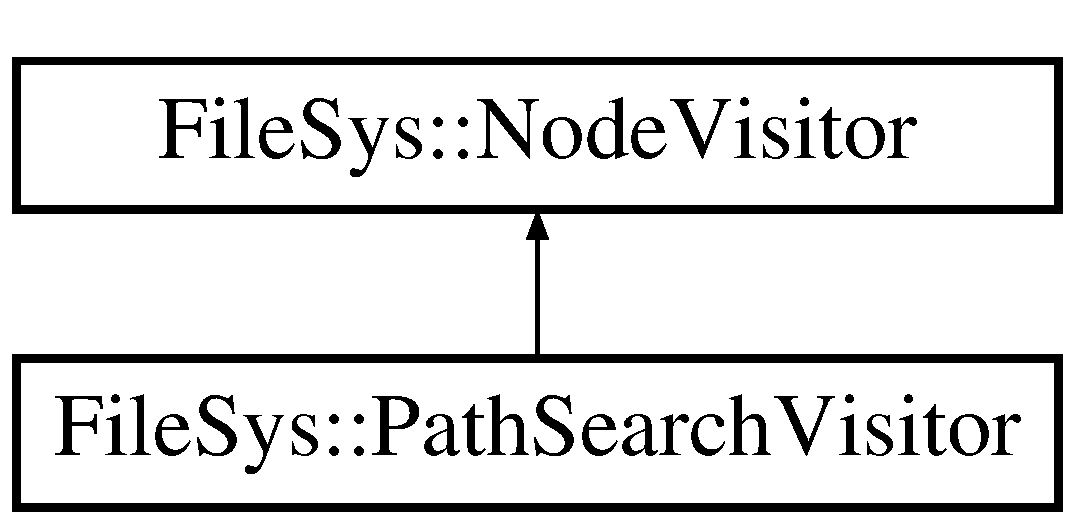
\includegraphics[height=2.000000cm]{class_file_sys_1_1_path_search_visitor}
\end{center}
\end{figure}
\subsection*{Public 成员函数}
\begin{DoxyCompactItemize}
\item 
virtual void \hyperlink{class_file_sys_1_1_path_search_visitor_ac9e8ab4c8389b118ba6a57b053ac8005}{Visit} (\hyperlink{class_file_sys_1_1_node}{Node} $\ast$node)
\begin{DoxyCompactList}\small\item\em 访问节点 \end{DoxyCompactList}\end{DoxyCompactItemize}
\subsection*{额外继承的成员函数}


\subsection{详细描述}


在文件 Path\-Search\-Visitor.\-h 第 10 行定义.



\subsection{成员函数说明}
\hypertarget{class_file_sys_1_1_path_search_visitor_ac9e8ab4c8389b118ba6a57b053ac8005}{\index{File\-Sys\-::\-Path\-Search\-Visitor@{File\-Sys\-::\-Path\-Search\-Visitor}!Visit@{Visit}}
\index{Visit@{Visit}!FileSys::PathSearchVisitor@{File\-Sys\-::\-Path\-Search\-Visitor}}
\subsubsection[{Visit}]{\setlength{\rightskip}{0pt plus 5cm}void File\-Sys\-::\-Path\-Search\-Visitor\-::\-Visit (
\begin{DoxyParamCaption}
\item[{{\bf Node} $\ast$}]{node}
\end{DoxyParamCaption}
)\hspace{0.3cm}{\ttfamily [virtual]}}}\label{class_file_sys_1_1_path_search_visitor_ac9e8ab4c8389b118ba6a57b053ac8005}


访问节点 


\begin{DoxyParams}{参数}
{\em node} & 待访问节点 \\
\hline
\end{DoxyParams}


重载 \hyperlink{class_file_sys_1_1_node_visitor_a3398560bc10e71a0b8fcaac57e5b58e2}{File\-Sys\-::\-Node\-Visitor} .



在文件 Path\-Search\-Visitor.\-cpp 第 17 行定义.



该类的文档由以下文件生成\-:\begin{DoxyCompactItemize}
\item 
Virtual\-Disk\-Console/Path\-Search\-Visitor.\-h\item 
Virtual\-Disk\-Console/Path\-Search\-Visitor.\-cpp\end{DoxyCompactItemize}

\hypertarget{class_util_1_1_queue_t}{\section{Util\-:\-:Queue\-T$<$ T $>$ 模板类 参考}
\label{class_util_1_1_queue_t}\index{Util\-::\-Queue\-T$<$ T $>$@{Util\-::\-Queue\-T$<$ T $>$}}
}
\subsection*{Public 成员函数}
\begin{DoxyCompactItemize}
\item 
\hypertarget{class_util_1_1_queue_t_a7f7dd7b295f6c8c32bcb14e7ab8370c3}{\hyperlink{class_util_1_1_queue_t_a7f7dd7b295f6c8c32bcb14e7ab8370c3}{Queue\-T} ()}\label{class_util_1_1_queue_t_a7f7dd7b295f6c8c32bcb14e7ab8370c3}

\begin{DoxyCompactList}\small\item\em 默认构造函数 \end{DoxyCompactList}\item 
\hypertarget{class_util_1_1_queue_t_a60ba7fd4b5b60e073e1c51a37dec811a}{\hyperlink{class_util_1_1_queue_t_a60ba7fd4b5b60e073e1c51a37dec811a}{Queue\-T} (const \hyperlink{class_util_1_1_queue_t}{Queue\-T} \&q)}\label{class_util_1_1_queue_t_a60ba7fd4b5b60e073e1c51a37dec811a}

\begin{DoxyCompactList}\small\item\em 拷贝构造函数 \end{DoxyCompactList}\item 
\hypertarget{class_util_1_1_queue_t_a87d170c71234c2076e219f49173b8f10}{\hyperlink{class_util_1_1_queue_t_a87d170c71234c2076e219f49173b8f10}{$\sim$\-Queue\-T} ()}\label{class_util_1_1_queue_t_a87d170c71234c2076e219f49173b8f10}

\begin{DoxyCompactList}\small\item\em 析构函数 \end{DoxyCompactList}\item 
void \hyperlink{class_util_1_1_queue_t_a77641ed829b14f0700d547ca1f4ee5ee}{Enqueue} (const T \&data)
\begin{DoxyCompactList}\small\item\em 将元素 data 入队列 \end{DoxyCompactList}\item 
\hypertarget{class_util_1_1_queue_t_a92cabe296935e24b22e9264a53d05892}{void \hyperlink{class_util_1_1_queue_t_a92cabe296935e24b22e9264a53d05892}{Dequeue} (void)}\label{class_util_1_1_queue_t_a92cabe296935e24b22e9264a53d05892}

\begin{DoxyCompactList}\small\item\em 将元素出队列 \end{DoxyCompactList}\item 
T \& \hyperlink{class_util_1_1_queue_t_a3feed3273640d0543f722e0a54d01bab}{Front} (void)
\begin{DoxyCompactList}\small\item\em 返回队列头部的元素 \end{DoxyCompactList}\item 
const T \& \hyperlink{class_util_1_1_queue_t_a8076426290e6d5750f2fe651620395b7}{Front} (void) const 
\begin{DoxyCompactList}\small\item\em 返回队列头部的元素 \end{DoxyCompactList}\item 
int \hyperlink{class_util_1_1_queue_t_a2f6575c0e530bb48b92537bbb37350d9}{Size} (void) const 
\begin{DoxyCompactList}\small\item\em 返回队列大小 \end{DoxyCompactList}\item 
\hyperlink{class_util_1_1_queue_t}{Queue\-T} \& \hyperlink{class_util_1_1_queue_t_a803f29fc2220ea056dcac90f3fce406f}{operator=} (const \hyperlink{class_util_1_1_queue_t}{Queue\-T} \&rhs)
\begin{DoxyCompactList}\small\item\em 赋值运算符重载 \end{DoxyCompactList}\end{DoxyCompactItemize}


\subsection{详细描述}
\subsubsection*{template$<$typename T$>$class Util\-::\-Queue\-T$<$ T $>$}



在文件 Queue.\-h 第 9 行定义.



\subsection{成员函数说明}
\hypertarget{class_util_1_1_queue_t_a77641ed829b14f0700d547ca1f4ee5ee}{\index{Util\-::\-Queue\-T@{Util\-::\-Queue\-T}!Enqueue@{Enqueue}}
\index{Enqueue@{Enqueue}!Util::QueueT@{Util\-::\-Queue\-T}}
\subsubsection[{Enqueue}]{\setlength{\rightskip}{0pt plus 5cm}template$<$typename T$>$ void {\bf Util\-::\-Queue\-T}$<$ T $>$\-::Enqueue (
\begin{DoxyParamCaption}
\item[{const T \&}]{data}
\end{DoxyParamCaption}
)\hspace{0.3cm}{\ttfamily [inline]}}}\label{class_util_1_1_queue_t_a77641ed829b14f0700d547ca1f4ee5ee}


将元素 data 入队列 


\begin{DoxyParams}{参数}
{\em data} & 要压入的元素 \\
\hline
\end{DoxyParams}


在文件 Queue.\-h 第 29 行定义.

\hypertarget{class_util_1_1_queue_t_a3feed3273640d0543f722e0a54d01bab}{\index{Util\-::\-Queue\-T@{Util\-::\-Queue\-T}!Front@{Front}}
\index{Front@{Front}!Util::QueueT@{Util\-::\-Queue\-T}}
\subsubsection[{Front}]{\setlength{\rightskip}{0pt plus 5cm}template$<$typename T$>$ T\& {\bf Util\-::\-Queue\-T}$<$ T $>$\-::Front (
\begin{DoxyParamCaption}
\item[{void}]{}
\end{DoxyParamCaption}
)\hspace{0.3cm}{\ttfamily [inline]}}}\label{class_util_1_1_queue_t_a3feed3273640d0543f722e0a54d01bab}


返回队列头部的元素 

\begin{DoxyReturn}{返回}
返回的队列头部元素 
\end{DoxyReturn}


在文件 Queue.\-h 第 40 行定义.

\hypertarget{class_util_1_1_queue_t_a8076426290e6d5750f2fe651620395b7}{\index{Util\-::\-Queue\-T@{Util\-::\-Queue\-T}!Front@{Front}}
\index{Front@{Front}!Util::QueueT@{Util\-::\-Queue\-T}}
\subsubsection[{Front}]{\setlength{\rightskip}{0pt plus 5cm}template$<$typename T$>$ const T\& {\bf Util\-::\-Queue\-T}$<$ T $>$\-::Front (
\begin{DoxyParamCaption}
\item[{void}]{}
\end{DoxyParamCaption}
) const\hspace{0.3cm}{\ttfamily [inline]}}}\label{class_util_1_1_queue_t_a8076426290e6d5750f2fe651620395b7}


返回队列头部的元素 

\begin{DoxyReturn}{返回}
返回的队列头部元素 
\end{DoxyReturn}


在文件 Queue.\-h 第 46 行定义.

\hypertarget{class_util_1_1_queue_t_a803f29fc2220ea056dcac90f3fce406f}{\index{Util\-::\-Queue\-T@{Util\-::\-Queue\-T}!operator=@{operator=}}
\index{operator=@{operator=}!Util::QueueT@{Util\-::\-Queue\-T}}
\subsubsection[{operator=}]{\setlength{\rightskip}{0pt plus 5cm}template$<$typename T$>$ {\bf Queue\-T}\& {\bf Util\-::\-Queue\-T}$<$ T $>$\-::operator= (
\begin{DoxyParamCaption}
\item[{const {\bf Queue\-T}$<$ T $>$ \&}]{rhs}
\end{DoxyParamCaption}
)\hspace{0.3cm}{\ttfamily [inline]}}}\label{class_util_1_1_queue_t_a803f29fc2220ea056dcac90f3fce406f}


赋值运算符重载 

\begin{DoxyReturn}{返回}
当前队列引用 
\end{DoxyReturn}


在文件 Queue.\-h 第 58 行定义.

\hypertarget{class_util_1_1_queue_t_a2f6575c0e530bb48b92537bbb37350d9}{\index{Util\-::\-Queue\-T@{Util\-::\-Queue\-T}!Size@{Size}}
\index{Size@{Size}!Util::QueueT@{Util\-::\-Queue\-T}}
\subsubsection[{Size}]{\setlength{\rightskip}{0pt plus 5cm}template$<$typename T$>$ int {\bf Util\-::\-Queue\-T}$<$ T $>$\-::Size (
\begin{DoxyParamCaption}
\item[{void}]{}
\end{DoxyParamCaption}
) const\hspace{0.3cm}{\ttfamily [inline]}}}\label{class_util_1_1_queue_t_a2f6575c0e530bb48b92537bbb37350d9}


返回队列大小 

\begin{DoxyReturn}{返回}
队列元素数 
\end{DoxyReturn}


在文件 Queue.\-h 第 52 行定义.



该类的文档由以下文件生成\-:\begin{DoxyCompactItemize}
\item 
Virtual\-Disk\-Console/Queue.\-h\end{DoxyCompactItemize}

\hypertarget{class_command_sys_1_1_rmdir_cmd}{\section{Command\-Sys\-:\-:Rmdir\-Cmd类 参考}
\label{class_command_sys_1_1_rmdir_cmd}\index{Command\-Sys\-::\-Rmdir\-Cmd@{Command\-Sys\-::\-Rmdir\-Cmd}}
}
类 Command\-Sys\-:\-:Rmdir\-Cmd 继承关系图\-:\begin{figure}[H]
\begin{center}
\leavevmode
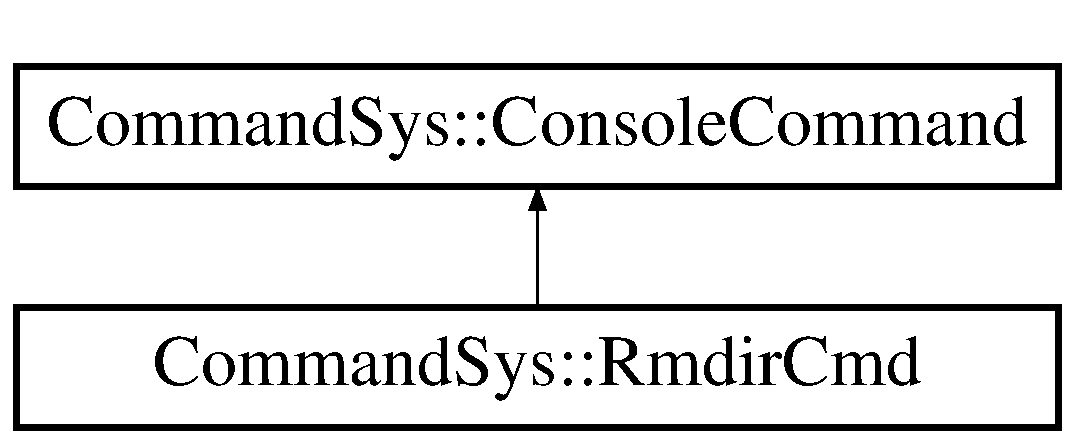
\includegraphics[height=2.000000cm]{class_command_sys_1_1_rmdir_cmd}
\end{center}
\end{figure}
\subsection*{Public 成员函数}
\begin{DoxyCompactItemize}
\item 
virtual void \hyperlink{class_command_sys_1_1_rmdir_cmd_a66d3b433eecba42b9f00f7fc3f09f623}{Execute} (void)
\begin{DoxyCompactList}\small\item\em 执行命令 \end{DoxyCompactList}\item 
\hypertarget{class_command_sys_1_1_rmdir_cmd_a112e65f47f834b1ee9b1cadd758378d6}{virtual void {\bfseries Delete\-This} (void)}\label{class_command_sys_1_1_rmdir_cmd_a112e65f47f834b1ee9b1cadd758378d6}

\end{DoxyCompactItemize}
\subsection*{额外继承的成员函数}


\subsection{详细描述}


在文件 Rmdir\-Cmd.\-h 第 9 行定义.



\subsection{成员函数说明}
\hypertarget{class_command_sys_1_1_rmdir_cmd_a66d3b433eecba42b9f00f7fc3f09f623}{\index{Command\-Sys\-::\-Rmdir\-Cmd@{Command\-Sys\-::\-Rmdir\-Cmd}!Execute@{Execute}}
\index{Execute@{Execute}!CommandSys::RmdirCmd@{Command\-Sys\-::\-Rmdir\-Cmd}}
\subsubsection[{Execute}]{\setlength{\rightskip}{0pt plus 5cm}void Command\-Sys\-::\-Rmdir\-Cmd\-::\-Execute (
\begin{DoxyParamCaption}
\item[{void}]{}
\end{DoxyParamCaption}
)\hspace{0.3cm}{\ttfamily [virtual]}}}\label{class_command_sys_1_1_rmdir_cmd_a66d3b433eecba42b9f00f7fc3f09f623}


执行命令 

\begin{DoxyRemark}{备注}
子类需重写该函数 
\end{DoxyRemark}


重载 \hyperlink{class_command_sys_1_1_console_command_a1d63e6780d3cfe83cc3452b0d797324c}{Command\-Sys\-::\-Console\-Command} .



在文件 Rmdir\-Cmd.\-cpp 第 15 行定义.



该类的文档由以下文件生成\-:\begin{DoxyCompactItemize}
\item 
Virtual\-Disk\-Console/Rmdir\-Cmd.\-h\item 
Virtual\-Disk\-Console/Rmdir\-Cmd.\-cpp\end{DoxyCompactItemize}

\hypertarget{class_lexer_sys_1_1_search_path}{\section{Lexer\-Sys\-:\-:Search\-Path类 参考}
\label{class_lexer_sys_1_1_search_path}\index{Lexer\-Sys\-::\-Search\-Path@{Lexer\-Sys\-::\-Search\-Path}}
}
\subsection*{Public 成员函数}
\begin{DoxyCompactItemize}
\item 
\hypertarget{class_lexer_sys_1_1_search_path_acb5047afe4efb653d8677f1646fa1c2b}{\hyperlink{class_lexer_sys_1_1_search_path_acb5047afe4efb653d8677f1646fa1c2b}{Search\-Path} (void)}\label{class_lexer_sys_1_1_search_path_acb5047afe4efb653d8677f1646fa1c2b}

\begin{DoxyCompactList}\small\item\em 默认构造函数 \end{DoxyCompactList}\item 
\hyperlink{class_lexer_sys_1_1_search_path_aba07d38fd89152b454fac47c5a6f000e}{Search\-Path} (const Util\-::\-String path)
\begin{DoxyCompactList}\small\item\em 带参数的构造函数 \end{DoxyCompactList}\item 
\hypertarget{class_lexer_sys_1_1_search_path_a8b67d627c73c4a278c82705cbadf5b8a}{\hyperlink{class_lexer_sys_1_1_search_path_a8b67d627c73c4a278c82705cbadf5b8a}{Search\-Path} (const \hyperlink{class_lexer_sys_1_1_search_path}{Search\-Path} \&path)}\label{class_lexer_sys_1_1_search_path_a8b67d627c73c4a278c82705cbadf5b8a}

\begin{DoxyCompactList}\small\item\em 拷贝构造函数 \end{DoxyCompactList}\item 
\hypertarget{class_lexer_sys_1_1_search_path_ac012486c06a45cf608f7fb101fb79520}{virtual \hyperlink{class_lexer_sys_1_1_search_path_ac012486c06a45cf608f7fb101fb79520}{$\sim$\-Search\-Path} (void)}\label{class_lexer_sys_1_1_search_path_ac012486c06a45cf608f7fb101fb79520}

\begin{DoxyCompactList}\small\item\em 析构函数 \end{DoxyCompactList}\item 
void \hyperlink{class_lexer_sys_1_1_search_path_a28ea29a96f8ef4c94f98d39c756b82f9}{Path} (const Util\-::\-String \&path)
\begin{DoxyCompactList}\small\item\em 设置路径 \end{DoxyCompactList}\item 
\hypertarget{class_lexer_sys_1_1_search_path_a0383fa9524f999a5905b1bac0beb1086}{Util\-::\-String \hyperlink{class_lexer_sys_1_1_search_path_a0383fa9524f999a5905b1bac0beb1086}{Path} (void) const }\label{class_lexer_sys_1_1_search_path_a0383fa9524f999a5905b1bac0beb1086}

\begin{DoxyCompactList}\small\item\em 返回路径名 \end{DoxyCompactList}\item 
\hypertarget{class_lexer_sys_1_1_search_path_a4f7a3ba73b0a7492cdace4e6dd28b0aa}{bool \hyperlink{class_lexer_sys_1_1_search_path_a4f7a3ba73b0a7492cdace4e6dd28b0aa}{Is\-Length\-Out\-Of\-Limit} (void) const }\label{class_lexer_sys_1_1_search_path_a4f7a3ba73b0a7492cdace4e6dd28b0aa}

\begin{DoxyCompactList}\small\item\em 查看路径是否超过长度限制 \end{DoxyCompactList}\item 
\hypertarget{class_lexer_sys_1_1_search_path_ac397ddb4bae3a2dcea86a07349f29dcc}{bool \hyperlink{class_lexer_sys_1_1_search_path_ac397ddb4bae3a2dcea86a07349f29dcc}{Get\-File\-Name\-Token} (\hyperlink{class_lexer_sys_1_1_token}{Token} \&tok)}\label{class_lexer_sys_1_1_search_path_ac397ddb4bae3a2dcea86a07349f29dcc}

\begin{DoxyCompactList}\small\item\em 返回路径中的文件名符号 \end{DoxyCompactList}\item 
\hypertarget{class_lexer_sys_1_1_search_path_a5f4a840231355612882f9a5775c836d6}{bool \hyperlink{class_lexer_sys_1_1_search_path_a5f4a840231355612882f9a5775c836d6}{Get\-Wild\-Card\-Token} (\hyperlink{class_lexer_sys_1_1_token}{Token} \&tok)}\label{class_lexer_sys_1_1_search_path_a5f4a840231355612882f9a5775c836d6}

\begin{DoxyCompactList}\small\item\em 返回路径名中的通配符 \end{DoxyCompactList}\item 
\hypertarget{class_lexer_sys_1_1_search_path_ae059c94615298f4018b35f8ac880ed9c}{bool \hyperlink{class_lexer_sys_1_1_search_path_ae059c94615298f4018b35f8ac880ed9c}{Is\-Empty} (void) const }\label{class_lexer_sys_1_1_search_path_ae059c94615298f4018b35f8ac880ed9c}

\begin{DoxyCompactList}\small\item\em 查看当前路径是否为空 \end{DoxyCompactList}\item 
\hypertarget{class_lexer_sys_1_1_search_path_acd045f1fae1586fe5f88d62162767640}{void \hyperlink{class_lexer_sys_1_1_search_path_acd045f1fae1586fe5f88d62162767640}{Clear} (void)}\label{class_lexer_sys_1_1_search_path_acd045f1fae1586fe5f88d62162767640}

\begin{DoxyCompactList}\small\item\em 清空路径 \end{DoxyCompactList}\item 
\hyperlink{class_lexer_sys_1_1_search_path}{Search\-Path} \& \hyperlink{class_lexer_sys_1_1_search_path_acfce5c8a697fbc69b09d3dcb29a00db1}{Append} (const \hyperlink{class_lexer_sys_1_1_search_path}{Search\-Path} \&path)
\begin{DoxyCompactList}\small\item\em 附加路径到此路径末尾 \end{DoxyCompactList}\item 
\hyperlink{class_lexer_sys_1_1_token}{Token} \& \hyperlink{class_lexer_sys_1_1_search_path_a47aaaf5b54a56d66516c6d4ad48ee9ae}{At} (const int i)
\begin{DoxyCompactList}\small\item\em 返回所在位置i处的符号 \end{DoxyCompactList}\item 
const \hyperlink{class_lexer_sys_1_1_token}{Token} \& \hyperlink{class_lexer_sys_1_1_search_path_a7dbfa28d64f9f2c83526d3e99d38a1cb}{At} (const int i) const 
\begin{DoxyCompactList}\small\item\em 返回所在位置i处的符号 \end{DoxyCompactList}\item 
int \hyperlink{class_lexer_sys_1_1_search_path_ae5331a0f6dc2934e37c4fc4684a70c09}{Token\-Count} (void) const 
\begin{DoxyCompactList}\small\item\em 当前路径的符号数量 \end{DoxyCompactList}\item 
bool \hyperlink{class_lexer_sys_1_1_search_path_a68b4a32eade0158303e8570811c6af2d}{Is\-Absolute\-Path} (void) const 
\begin{DoxyCompactList}\small\item\em 分析当前路径是否为绝对路径 \end{DoxyCompactList}\item 
bool \hyperlink{class_lexer_sys_1_1_search_path_a83f7615804a9fac015e0434ab183d09e}{Curr\-Token} (\hyperlink{class_lexer_sys_1_1_token}{Token} \&tok) const 
\begin{DoxyCompactList}\small\item\em 遍历该路径各符号结点时的当前符号 \end{DoxyCompactList}\item 
\hypertarget{class_lexer_sys_1_1_search_path_a489e6a5e1491504d3c30d0521694ac68}{bool \hyperlink{class_lexer_sys_1_1_search_path_a489e6a5e1491504d3c30d0521694ac68}{Has\-Next} (void) const }\label{class_lexer_sys_1_1_search_path_a489e6a5e1491504d3c30d0521694ac68}

\begin{DoxyCompactList}\small\item\em 是否含有下一个符号 \end{DoxyCompactList}\item 
\hypertarget{class_lexer_sys_1_1_search_path_aa5e2c3b515e1b2ca4c4d8cfbc5987c3a}{void \hyperlink{class_lexer_sys_1_1_search_path_aa5e2c3b515e1b2ca4c4d8cfbc5987c3a}{Move\-To\-First\-Token} (void)}\label{class_lexer_sys_1_1_search_path_aa5e2c3b515e1b2ca4c4d8cfbc5987c3a}

\begin{DoxyCompactList}\small\item\em 将当前符号位置移动到符号列表首 \end{DoxyCompactList}\item 
\hypertarget{class_lexer_sys_1_1_search_path_a8db4727a6247e8c8cfac5d04b30270cb}{void \hyperlink{class_lexer_sys_1_1_search_path_a8db4727a6247e8c8cfac5d04b30270cb}{Move\-To\-Next\-Token} (void)}\label{class_lexer_sys_1_1_search_path_a8db4727a6247e8c8cfac5d04b30270cb}

\begin{DoxyCompactList}\small\item\em 将当前符号位置移动到下一个符号位置 \end{DoxyCompactList}\item 
\hypertarget{class_lexer_sys_1_1_search_path_aa7e29634b570628decaa7375a3ee1b33}{void \hyperlink{class_lexer_sys_1_1_search_path_aa7e29634b570628decaa7375a3ee1b33}{Move\-To\-Last\-Token} (void)}\label{class_lexer_sys_1_1_search_path_aa7e29634b570628decaa7375a3ee1b33}

\begin{DoxyCompactList}\small\item\em 将当前符号位置移动到最后一个符号位置 \end{DoxyCompactList}\item 
\hypertarget{class_lexer_sys_1_1_search_path_a53eb16d1e0630183e842c9a8b597b98b}{\hyperlink{class_lexer_sys_1_1_search_path}{Search\-Path} \& \hyperlink{class_lexer_sys_1_1_search_path_a53eb16d1e0630183e842c9a8b597b98b}{operator=} (const \hyperlink{class_lexer_sys_1_1_search_path}{Search\-Path} \&rhs)}\label{class_lexer_sys_1_1_search_path_a53eb16d1e0630183e842c9a8b597b98b}

\begin{DoxyCompactList}\small\item\em 赋值运算符重载 \end{DoxyCompactList}\item 
\hypertarget{class_lexer_sys_1_1_search_path_ab5e4e94635679d471b24b92379957623}{\hyperlink{class_lexer_sys_1_1_search_path}{Search\-Path} \& \hyperlink{class_lexer_sys_1_1_search_path_ab5e4e94635679d471b24b92379957623}{operator=} (const Util\-::\-String \&rhs)}\label{class_lexer_sys_1_1_search_path_ab5e4e94635679d471b24b92379957623}

\begin{DoxyCompactList}\small\item\em 赋值运算符重载 \end{DoxyCompactList}\end{DoxyCompactItemize}
\subsection*{Protected 成员函数}
\begin{DoxyCompactItemize}
\item 
\hypertarget{class_lexer_sys_1_1_search_path_aad51779844ceaa5c0cb04be7c3481007}{void \hyperlink{class_lexer_sys_1_1_search_path_aad51779844ceaa5c0cb04be7c3481007}{Analysis\-Path} (void)}\label{class_lexer_sys_1_1_search_path_aad51779844ceaa5c0cb04be7c3481007}

\begin{DoxyCompactList}\small\item\em 从路径名中分析出符号并存入传入的符号链表中 \end{DoxyCompactList}\end{DoxyCompactItemize}


\subsection{详细描述}


在文件 Search\-Path.\-h 第 13 行定义.



\subsection{构造及析构函数说明}
\hypertarget{class_lexer_sys_1_1_search_path_aba07d38fd89152b454fac47c5a6f000e}{\index{Lexer\-Sys\-::\-Search\-Path@{Lexer\-Sys\-::\-Search\-Path}!Search\-Path@{Search\-Path}}
\index{Search\-Path@{Search\-Path}!LexerSys::SearchPath@{Lexer\-Sys\-::\-Search\-Path}}
\subsubsection[{Search\-Path}]{\setlength{\rightskip}{0pt plus 5cm}Lexer\-Sys\-::\-Search\-Path\-::\-Search\-Path (
\begin{DoxyParamCaption}
\item[{const Util\-::\-String}]{path}
\end{DoxyParamCaption}
)}}\label{class_lexer_sys_1_1_search_path_aba07d38fd89152b454fac47c5a6f000e}


带参数的构造函数 


\begin{DoxyParams}{参数}
{\em path} & 要设置的路径字符串 \\
\hline
\end{DoxyParams}


在文件 Search\-Path.\-cpp 第 19 行定义.



\subsection{成员函数说明}
\hypertarget{class_lexer_sys_1_1_search_path_acfce5c8a697fbc69b09d3dcb29a00db1}{\index{Lexer\-Sys\-::\-Search\-Path@{Lexer\-Sys\-::\-Search\-Path}!Append@{Append}}
\index{Append@{Append}!LexerSys::SearchPath@{Lexer\-Sys\-::\-Search\-Path}}
\subsubsection[{Append}]{\setlength{\rightskip}{0pt plus 5cm}{\bf Search\-Path} \& Lexer\-Sys\-::\-Search\-Path\-::\-Append (
\begin{DoxyParamCaption}
\item[{const {\bf Search\-Path} \&}]{path}
\end{DoxyParamCaption}
)}}\label{class_lexer_sys_1_1_search_path_acfce5c8a697fbc69b09d3dcb29a00db1}


附加路径到此路径末尾 


\begin{DoxyParams}{参数}
{\em path} & 要附加的路径 \\
\hline
\end{DoxyParams}
\begin{DoxyReturn}{返回}
返回当前路径引用 
\end{DoxyReturn}


在文件 Search\-Path.\-cpp 第 164 行定义.

\hypertarget{class_lexer_sys_1_1_search_path_a47aaaf5b54a56d66516c6d4ad48ee9ae}{\index{Lexer\-Sys\-::\-Search\-Path@{Lexer\-Sys\-::\-Search\-Path}!At@{At}}
\index{At@{At}!LexerSys::SearchPath@{Lexer\-Sys\-::\-Search\-Path}}
\subsubsection[{At}]{\setlength{\rightskip}{0pt plus 5cm}{\bf Token} \& Lexer\-Sys\-::\-Search\-Path\-::\-At (
\begin{DoxyParamCaption}
\item[{const int}]{i}
\end{DoxyParamCaption}
)}}\label{class_lexer_sys_1_1_search_path_a47aaaf5b54a56d66516c6d4ad48ee9ae}


返回所在位置i处的符号 


\begin{DoxyParams}{参数}
{\em i} & 位置索引 \\
\hline
\end{DoxyParams}
\begin{DoxyReturn}{返回}
所在位置的符号 
\end{DoxyReturn}


在文件 Search\-Path.\-cpp 第 40 行定义.

\hypertarget{class_lexer_sys_1_1_search_path_a7dbfa28d64f9f2c83526d3e99d38a1cb}{\index{Lexer\-Sys\-::\-Search\-Path@{Lexer\-Sys\-::\-Search\-Path}!At@{At}}
\index{At@{At}!LexerSys::SearchPath@{Lexer\-Sys\-::\-Search\-Path}}
\subsubsection[{At}]{\setlength{\rightskip}{0pt plus 5cm}const {\bf Token} \& Lexer\-Sys\-::\-Search\-Path\-::\-At (
\begin{DoxyParamCaption}
\item[{const int}]{i}
\end{DoxyParamCaption}
) const}}\label{class_lexer_sys_1_1_search_path_a7dbfa28d64f9f2c83526d3e99d38a1cb}


返回所在位置i处的符号 


\begin{DoxyParams}{参数}
{\em i} & 位置索引 \\
\hline
\end{DoxyParams}
\begin{DoxyReturn}{返回}
所在位置的符号 
\end{DoxyReturn}


在文件 Search\-Path.\-cpp 第 45 行定义.

\hypertarget{class_lexer_sys_1_1_search_path_a83f7615804a9fac015e0434ab183d09e}{\index{Lexer\-Sys\-::\-Search\-Path@{Lexer\-Sys\-::\-Search\-Path}!Curr\-Token@{Curr\-Token}}
\index{Curr\-Token@{Curr\-Token}!LexerSys::SearchPath@{Lexer\-Sys\-::\-Search\-Path}}
\subsubsection[{Curr\-Token}]{\setlength{\rightskip}{0pt plus 5cm}bool Lexer\-Sys\-::\-Search\-Path\-::\-Curr\-Token (
\begin{DoxyParamCaption}
\item[{{\bf Token} \&}]{tok}
\end{DoxyParamCaption}
) const}}\label{class_lexer_sys_1_1_search_path_a83f7615804a9fac015e0434ab183d09e}


遍历该路径各符号结点时的当前符号 


\begin{DoxyParams}{参数}
{\em 获取的当前符号} & \\
\hline
\end{DoxyParams}
\begin{DoxyReturn}{返回}
获取是否成功 
\end{DoxyReturn}

\begin{DoxyRetVals}{返回值}
{\em true} & 获取成功 \\
\hline
{\em false} & 获取失败 \\
\hline
\end{DoxyRetVals}


在文件 Search\-Path.\-cpp 第 50 行定义.

\hypertarget{class_lexer_sys_1_1_search_path_a68b4a32eade0158303e8570811c6af2d}{\index{Lexer\-Sys\-::\-Search\-Path@{Lexer\-Sys\-::\-Search\-Path}!Is\-Absolute\-Path@{Is\-Absolute\-Path}}
\index{Is\-Absolute\-Path@{Is\-Absolute\-Path}!LexerSys::SearchPath@{Lexer\-Sys\-::\-Search\-Path}}
\subsubsection[{Is\-Absolute\-Path}]{\setlength{\rightskip}{0pt plus 5cm}bool Lexer\-Sys\-::\-Search\-Path\-::\-Is\-Absolute\-Path (
\begin{DoxyParamCaption}
\item[{void}]{}
\end{DoxyParamCaption}
) const}}\label{class_lexer_sys_1_1_search_path_a68b4a32eade0158303e8570811c6af2d}


分析当前路径是否为绝对路径 


\begin{DoxyParams}{参数}
{\em toks} & 待分析路径符号列表 \\
\hline
\end{DoxyParams}
\begin{DoxyReturn}{返回}
返回是否为绝对路径 
\end{DoxyReturn}


在文件 Search\-Path.\-cpp 第 147 行定义.

\hypertarget{class_lexer_sys_1_1_search_path_a28ea29a96f8ef4c94f98d39c756b82f9}{\index{Lexer\-Sys\-::\-Search\-Path@{Lexer\-Sys\-::\-Search\-Path}!Path@{Path}}
\index{Path@{Path}!LexerSys::SearchPath@{Lexer\-Sys\-::\-Search\-Path}}
\subsubsection[{Path}]{\setlength{\rightskip}{0pt plus 5cm}void Lexer\-Sys\-::\-Search\-Path\-::\-Path (
\begin{DoxyParamCaption}
\item[{const Util\-::\-String \&}]{path}
\end{DoxyParamCaption}
)}}\label{class_lexer_sys_1_1_search_path_a28ea29a96f8ef4c94f98d39c756b82f9}


设置路径 


\begin{DoxyParams}{参数}
{\em path} & 路径字符串 \\
\hline
\end{DoxyParams}
\begin{DoxyRemark}{备注}
该命令会将路径字符串分解为独立的符号。 
\end{DoxyRemark}


在文件 Search\-Path.\-cpp 第 28 行定义.

\hypertarget{class_lexer_sys_1_1_search_path_ae5331a0f6dc2934e37c4fc4684a70c09}{\index{Lexer\-Sys\-::\-Search\-Path@{Lexer\-Sys\-::\-Search\-Path}!Token\-Count@{Token\-Count}}
\index{Token\-Count@{Token\-Count}!LexerSys::SearchPath@{Lexer\-Sys\-::\-Search\-Path}}
\subsubsection[{Token\-Count}]{\setlength{\rightskip}{0pt plus 5cm}int Lexer\-Sys\-::\-Search\-Path\-::\-Token\-Count (
\begin{DoxyParamCaption}
\item[{void}]{}
\end{DoxyParamCaption}
) const}}\label{class_lexer_sys_1_1_search_path_ae5331a0f6dc2934e37c4fc4684a70c09}


当前路径的符号数量 

\begin{DoxyReturn}{返回}
当前路径所包含的符号数 
\end{DoxyReturn}


在文件 Search\-Path.\-cpp 第 60 行定义.



该类的文档由以下文件生成\-:\begin{DoxyCompactItemize}
\item 
Virtual\-Disk\-Console/Search\-Path.\-h\item 
Virtual\-Disk\-Console/Search\-Path.\-cpp\end{DoxyCompactItemize}

\hypertarget{class_util_1_1_singleton_t}{\section{Util\-:\-:Singleton\-T$<$ T $>$ 模板类 参考}
\label{class_util_1_1_singleton_t}\index{Util\-::\-Singleton\-T$<$ T $>$@{Util\-::\-Singleton\-T$<$ T $>$}}
}


{\ttfamily \#include $<$Singleton.\-h$>$}

\subsection*{静态 Public 成员函数}
\begin{DoxyCompactItemize}
\item 
static void \hyperlink{class_util_1_1_singleton_t_adc93fbaad3654ccfcbc568af60f79b83}{Create\-Instance} (void)
\begin{DoxyCompactList}\small\item\em 创建单例中的实例,全局只可在系统初始化时调用一次 \end{DoxyCompactList}\item 
static void \hyperlink{class_util_1_1_singleton_t_a57e01e60edc894293383bb1b6375e2a2}{Destroy\-Instance} (void)
\begin{DoxyCompactList}\small\item\em 销毁单例中的实例,全局在销毁单例时调用一次 \end{DoxyCompactList}\item 
static T $\ast$ \hyperlink{class_util_1_1_singleton_t_a977b19d9052e8d16cd5ed79d7d49d597}{Get\-Instance} (void)
\begin{DoxyCompactList}\small\item\em 获得实例指针 \end{DoxyCompactList}\end{DoxyCompactItemize}


\subsection{详细描述}
\subsubsection*{template$<$typename T$>$class Util\-::\-Singleton\-T$<$ T $>$}

此类为单例模板类 

在文件 Singleton.\-h 第 12 行定义.



\subsection{成员函数说明}
\hypertarget{class_util_1_1_singleton_t_adc93fbaad3654ccfcbc568af60f79b83}{\index{Util\-::\-Singleton\-T@{Util\-::\-Singleton\-T}!Create\-Instance@{Create\-Instance}}
\index{Create\-Instance@{Create\-Instance}!Util::SingletonT@{Util\-::\-Singleton\-T}}
\subsubsection[{Create\-Instance}]{\setlength{\rightskip}{0pt plus 5cm}template$<$typename T$>$ static void {\bf Util\-::\-Singleton\-T}$<$ T $>$\-::Create\-Instance (
\begin{DoxyParamCaption}
\item[{void}]{}
\end{DoxyParamCaption}
)\hspace{0.3cm}{\ttfamily [inline]}, {\ttfamily [static]}}}\label{class_util_1_1_singleton_t_adc93fbaad3654ccfcbc568af60f79b83}


创建单例中的实例,全局只可在系统初始化时调用一次 

\begin{DoxyWarning}{警告}
此函数全局只可调用一次,否则会触发断言 
\end{DoxyWarning}


在文件 Singleton.\-h 第 22 行定义.

\hypertarget{class_util_1_1_singleton_t_a57e01e60edc894293383bb1b6375e2a2}{\index{Util\-::\-Singleton\-T@{Util\-::\-Singleton\-T}!Destroy\-Instance@{Destroy\-Instance}}
\index{Destroy\-Instance@{Destroy\-Instance}!Util::SingletonT@{Util\-::\-Singleton\-T}}
\subsubsection[{Destroy\-Instance}]{\setlength{\rightskip}{0pt plus 5cm}template$<$typename T$>$ static void {\bf Util\-::\-Singleton\-T}$<$ T $>$\-::Destroy\-Instance (
\begin{DoxyParamCaption}
\item[{void}]{}
\end{DoxyParamCaption}
)\hspace{0.3cm}{\ttfamily [inline]}, {\ttfamily [static]}}}\label{class_util_1_1_singleton_t_a57e01e60edc894293383bb1b6375e2a2}


销毁单例中的实例,全局在销毁单例时调用一次 

\begin{DoxyWarning}{警告}
此函数必须在\-Create\-Instance调用后调用,否则会触发断言 
\end{DoxyWarning}


在文件 Singleton.\-h 第 33 行定义.

\hypertarget{class_util_1_1_singleton_t_a977b19d9052e8d16cd5ed79d7d49d597}{\index{Util\-::\-Singleton\-T@{Util\-::\-Singleton\-T}!Get\-Instance@{Get\-Instance}}
\index{Get\-Instance@{Get\-Instance}!Util::SingletonT@{Util\-::\-Singleton\-T}}
\subsubsection[{Get\-Instance}]{\setlength{\rightskip}{0pt plus 5cm}template$<$typename T$>$ static T$\ast$ {\bf Util\-::\-Singleton\-T}$<$ T $>$\-::Get\-Instance (
\begin{DoxyParamCaption}
\item[{void}]{}
\end{DoxyParamCaption}
)\hspace{0.3cm}{\ttfamily [inline]}, {\ttfamily [static]}}}\label{class_util_1_1_singleton_t_a977b19d9052e8d16cd5ed79d7d49d597}


获得实例指针 

\begin{DoxyReturn}{返回}
该单例的全局唯一实例指针 

返回全局该对象的唯一实例,此函数必须在\-Create\-Instance调用后调用 否则会触发断言 
\end{DoxyReturn}


在文件 Singleton.\-h 第 46 行定义.



该类的文档由以下文件生成\-:\begin{DoxyCompactItemize}
\item 
Virtual\-Disk\-Console/Singleton.\-h\end{DoxyCompactItemize}

\hypertarget{class_util_1_1_stack_t}{\section{Util\-:\-:Stack\-T$<$ T $>$ 模板类 参考}
\label{class_util_1_1_stack_t}\index{Util\-::\-Stack\-T$<$ T $>$@{Util\-::\-Stack\-T$<$ T $>$}}
}
\subsection*{Public 成员函数}
\begin{DoxyCompactItemize}
\item 
\hypertarget{class_util_1_1_stack_t_adbbf65f8d1cf6764a5578de90e3ad551}{\hyperlink{class_util_1_1_stack_t_adbbf65f8d1cf6764a5578de90e3ad551}{Stack\-T} (void)}\label{class_util_1_1_stack_t_adbbf65f8d1cf6764a5578de90e3ad551}

\begin{DoxyCompactList}\small\item\em 默认构造函数 \end{DoxyCompactList}\item 
\hypertarget{class_util_1_1_stack_t_a5731dcd6ca4aa9b0b6ef57c61633cf7e}{\hyperlink{class_util_1_1_stack_t_a5731dcd6ca4aa9b0b6ef57c61633cf7e}{Stack\-T} (const \hyperlink{class_util_1_1_stack_t}{Stack\-T} \&stack)}\label{class_util_1_1_stack_t_a5731dcd6ca4aa9b0b6ef57c61633cf7e}

\begin{DoxyCompactList}\small\item\em 拷贝构造函数 \end{DoxyCompactList}\item 
\hypertarget{class_util_1_1_stack_t_a1e3f88666426b8ddfbc6e76615f00dd4}{\hyperlink{class_util_1_1_stack_t_a1e3f88666426b8ddfbc6e76615f00dd4}{$\sim$\-Stack\-T} ()}\label{class_util_1_1_stack_t_a1e3f88666426b8ddfbc6e76615f00dd4}

\begin{DoxyCompactList}\small\item\em 析构函数 \end{DoxyCompactList}\item 
void \hyperlink{class_util_1_1_stack_t_af12278ddc72374d7d134828c6590ea7f}{Push} (const T \&data)
\begin{DoxyCompactList}\small\item\em 将元素data入栈 \end{DoxyCompactList}\item 
\hypertarget{class_util_1_1_stack_t_af3ee55adee3de52f9e88f8d0edd8dd71}{void \hyperlink{class_util_1_1_stack_t_af3ee55adee3de52f9e88f8d0edd8dd71}{Pop} (void)}\label{class_util_1_1_stack_t_af3ee55adee3de52f9e88f8d0edd8dd71}

\begin{DoxyCompactList}\small\item\em 将栈顶元素出栈 \end{DoxyCompactList}\item 
int \hyperlink{class_util_1_1_stack_t_a6f4a2b4e2664e9a771e989a31dbfa27d}{Size} (void) const 
\begin{DoxyCompactList}\small\item\em 返回栈元素数 \end{DoxyCompactList}\item 
bool \hyperlink{class_util_1_1_stack_t_a1a6fa3d62c05f1bf24b21924a6f692f0}{Is\-Empty} (void) const 
\begin{DoxyCompactList}\small\item\em 栈是否为空 \end{DoxyCompactList}\item 
T \& \hyperlink{class_util_1_1_stack_t_aab6508f39b4c9e364c492955b26273be}{Front} (void)
\begin{DoxyCompactList}\small\item\em 返回栈顶元素 \end{DoxyCompactList}\item 
const T \& \hyperlink{class_util_1_1_stack_t_ac298ea33edc7cd88fc9f640e39c8d9c7}{Front} (void) const 
\begin{DoxyCompactList}\small\item\em 返回栈顶元素 \end{DoxyCompactList}\item 
\hypertarget{class_util_1_1_stack_t_af093ce3aaa86e1807ed34e118c785cf9}{\hyperlink{class_util_1_1_stack_t}{Stack\-T} \& \hyperlink{class_util_1_1_stack_t_af093ce3aaa86e1807ed34e118c785cf9}{operator=} (const \hyperlink{class_util_1_1_stack_t}{Stack\-T} \&stack)}\label{class_util_1_1_stack_t_af093ce3aaa86e1807ed34e118c785cf9}

\begin{DoxyCompactList}\small\item\em 赋值运算符重载 \end{DoxyCompactList}\end{DoxyCompactItemize}


\subsection{详细描述}
\subsubsection*{template$<$typename T$>$class Util\-::\-Stack\-T$<$ T $>$}



在文件 Stack.\-h 第 9 行定义.



\subsection{成员函数说明}
\hypertarget{class_util_1_1_stack_t_aab6508f39b4c9e364c492955b26273be}{\index{Util\-::\-Stack\-T@{Util\-::\-Stack\-T}!Front@{Front}}
\index{Front@{Front}!Util::StackT@{Util\-::\-Stack\-T}}
\subsubsection[{Front}]{\setlength{\rightskip}{0pt plus 5cm}template$<$typename T$>$ T\& {\bf Util\-::\-Stack\-T}$<$ T $>$\-::Front (
\begin{DoxyParamCaption}
\item[{void}]{}
\end{DoxyParamCaption}
)\hspace{0.3cm}{\ttfamily [inline]}}}\label{class_util_1_1_stack_t_aab6508f39b4c9e364c492955b26273be}


返回栈顶元素 

\begin{DoxyReturn}{返回}
栈顶元素 
\end{DoxyReturn}


在文件 Stack.\-h 第 49 行定义.

\hypertarget{class_util_1_1_stack_t_ac298ea33edc7cd88fc9f640e39c8d9c7}{\index{Util\-::\-Stack\-T@{Util\-::\-Stack\-T}!Front@{Front}}
\index{Front@{Front}!Util::StackT@{Util\-::\-Stack\-T}}
\subsubsection[{Front}]{\setlength{\rightskip}{0pt plus 5cm}template$<$typename T$>$ const T\& {\bf Util\-::\-Stack\-T}$<$ T $>$\-::Front (
\begin{DoxyParamCaption}
\item[{void}]{}
\end{DoxyParamCaption}
) const\hspace{0.3cm}{\ttfamily [inline]}}}\label{class_util_1_1_stack_t_ac298ea33edc7cd88fc9f640e39c8d9c7}


返回栈顶元素 

\begin{DoxyReturn}{返回}
栈顶元素 
\end{DoxyReturn}


在文件 Stack.\-h 第 55 行定义.

\hypertarget{class_util_1_1_stack_t_a1a6fa3d62c05f1bf24b21924a6f692f0}{\index{Util\-::\-Stack\-T@{Util\-::\-Stack\-T}!Is\-Empty@{Is\-Empty}}
\index{Is\-Empty@{Is\-Empty}!Util::StackT@{Util\-::\-Stack\-T}}
\subsubsection[{Is\-Empty}]{\setlength{\rightskip}{0pt plus 5cm}template$<$typename T$>$ bool {\bf Util\-::\-Stack\-T}$<$ T $>$\-::Is\-Empty (
\begin{DoxyParamCaption}
\item[{void}]{}
\end{DoxyParamCaption}
) const\hspace{0.3cm}{\ttfamily [inline]}}}\label{class_util_1_1_stack_t_a1a6fa3d62c05f1bf24b21924a6f692f0}


栈是否为空 


\begin{DoxyRetVals}{返回值}
{\em true} & 栈为空栈 \\
\hline
{\em false} & 栈为非空 \\
\hline
\end{DoxyRetVals}


在文件 Stack.\-h 第 44 行定义.

\hypertarget{class_util_1_1_stack_t_af12278ddc72374d7d134828c6590ea7f}{\index{Util\-::\-Stack\-T@{Util\-::\-Stack\-T}!Push@{Push}}
\index{Push@{Push}!Util::StackT@{Util\-::\-Stack\-T}}
\subsubsection[{Push}]{\setlength{\rightskip}{0pt plus 5cm}template$<$typename T$>$ void {\bf Util\-::\-Stack\-T}$<$ T $>$\-::Push (
\begin{DoxyParamCaption}
\item[{const T \&}]{data}
\end{DoxyParamCaption}
)\hspace{0.3cm}{\ttfamily [inline]}}}\label{class_util_1_1_stack_t_af12278ddc72374d7d134828c6590ea7f}


将元素data入栈 


\begin{DoxyParams}{参数}
{\em data} & 要入栈元素 \\
\hline
\end{DoxyParams}


在文件 Stack.\-h 第 29 行定义.

\hypertarget{class_util_1_1_stack_t_a6f4a2b4e2664e9a771e989a31dbfa27d}{\index{Util\-::\-Stack\-T@{Util\-::\-Stack\-T}!Size@{Size}}
\index{Size@{Size}!Util::StackT@{Util\-::\-Stack\-T}}
\subsubsection[{Size}]{\setlength{\rightskip}{0pt plus 5cm}template$<$typename T$>$ int {\bf Util\-::\-Stack\-T}$<$ T $>$\-::Size (
\begin{DoxyParamCaption}
\item[{void}]{}
\end{DoxyParamCaption}
) const\hspace{0.3cm}{\ttfamily [inline]}}}\label{class_util_1_1_stack_t_a6f4a2b4e2664e9a771e989a31dbfa27d}


返回栈元素数 

\begin{DoxyReturn}{返回}
栈元素数 
\end{DoxyReturn}


在文件 Stack.\-h 第 38 行定义.



该类的文档由以下文件生成\-:\begin{DoxyCompactItemize}
\item 
Virtual\-Disk\-Console/Stack.\-h\end{DoxyCompactItemize}

\hypertarget{class_util_1_1_string_t}{\section{Util\-:\-:String\-T$<$ T $>$ 模板类 参考}
\label{class_util_1_1_string_t}\index{Util\-::\-String\-T$<$ T $>$@{Util\-::\-String\-T$<$ T $>$}}
}
\subsection*{Public 类型}
\begin{DoxyCompactItemize}
\item 
\hypertarget{class_util_1_1_string_t_a120efc2171f8e53732aa4b56d9ba37c6}{typedef T {\bfseries X\-C\-H\-A\-R}}\label{class_util_1_1_string_t_a120efc2171f8e53732aa4b56d9ba37c6}

\end{DoxyCompactItemize}
\subsection*{Public 成员函数}
\begin{DoxyCompactItemize}
\item 
\hypertarget{class_util_1_1_string_t_a883cbb1e8a0f3b732aca84b0d9cd266b}{\hyperlink{class_util_1_1_string_t_a883cbb1e8a0f3b732aca84b0d9cd266b}{String\-T} ()}\label{class_util_1_1_string_t_a883cbb1e8a0f3b732aca84b0d9cd266b}

\begin{DoxyCompactList}\small\item\em 默认构造函数 \end{DoxyCompactList}\item 
\hypertarget{class_util_1_1_string_t_aad980a5b36d5f16f6fea4c6630bb813d}{{\bfseries String\-T} (const T $\ast$str)}\label{class_util_1_1_string_t_aad980a5b36d5f16f6fea4c6630bb813d}

\item 
\hypertarget{class_util_1_1_string_t_a1257b8075074f19bb1c9814494b15068}{\hyperlink{class_util_1_1_string_t_a1257b8075074f19bb1c9814494b15068}{String\-T} (const \hyperlink{class_util_1_1_string_t}{String\-T} \&str)}\label{class_util_1_1_string_t_a1257b8075074f19bb1c9814494b15068}

\begin{DoxyCompactList}\small\item\em 拷贝构造函数 \end{DoxyCompactList}\item 
\hypertarget{class_util_1_1_string_t_abe51bcfdbfb0f1929d2c4cff929a8808}{\hyperlink{class_util_1_1_string_t_abe51bcfdbfb0f1929d2c4cff929a8808}{$\sim$\-String\-T} ()}\label{class_util_1_1_string_t_abe51bcfdbfb0f1929d2c4cff929a8808}

\begin{DoxyCompactList}\small\item\em 析构函数 \end{DoxyCompactList}\item 
void \hyperlink{class_util_1_1_string_t_a5775703e044ee57083e8dbed36837ec2}{Assign} (const int len)
\begin{DoxyCompactList}\small\item\em 根据所需字符串长度调整缓冲区大小 \end{DoxyCompactList}\item 
int \hyperlink{class_util_1_1_string_t_ab8dd0984514e44046b30f66e1f63b2c1}{Length} (void) const 
\begin{DoxyCompactList}\small\item\em 返回字符串长度 \end{DoxyCompactList}\item 
int \hyperlink{class_util_1_1_string_t_a72e976002115574ec303af27375ed65f}{Capacity} (void) const 
\begin{DoxyCompactList}\small\item\em 返回字符串缓冲区所能容纳的字符数 \end{DoxyCompactList}\item 
bool \hyperlink{class_util_1_1_string_t_a216aedf3b116d9f2b402edfd2d4f41c5}{Is\-Empty} (void) const 
\begin{DoxyCompactList}\small\item\em 返回当前字符串是否为空 \end{DoxyCompactList}\item 
T \& \hyperlink{class_util_1_1_string_t_a89a211d1470fce86db51e798137488b9}{At} (const int i)
\begin{DoxyCompactList}\small\item\em 返回索引处的字符 \end{DoxyCompactList}\item 
const T \& \hyperlink{class_util_1_1_string_t_a9dbec7dd16a3f3b30ec1c893fce410b2}{At} (const int i) const 
\begin{DoxyCompactList}\small\item\em 返回索引处的字符 \end{DoxyCompactList}\item 
int \hyperlink{class_util_1_1_string_t_ae3904115e9111e8254fea22fbd522fbb}{Delete} (const int i, const int len)
\begin{DoxyCompactList}\small\item\em 删除字符串中指定范围内的子字符串 \end{DoxyCompactList}\item 
\hyperlink{class_util_1_1_string_t}{String\-T} \& \hyperlink{class_util_1_1_string_t_a643a72c0f360c781ad27f0c1aaa9ce84}{Insert} (const \hyperlink{class_util_1_1_string_t}{String\-T} \&str, const int i)
\begin{DoxyCompactList}\small\item\em 在 i 处之前插入 str 字符串 \end{DoxyCompactList}\item 
int \hyperlink{class_util_1_1_string_t_ac5aba7f0da8bd71c812c3a609ccf4840}{Compare} (const \hyperlink{class_util_1_1_string_t}{String\-T} \&str, const bool lowercast=false) const 
\begin{DoxyCompactList}\small\item\em 传入字符串与当前字符串比较 \end{DoxyCompactList}\item 
int \hyperlink{class_util_1_1_string_t_a0f8cc8e5867626a77cb749f6d31ffd35}{I\-Cmp} (const \hyperlink{class_util_1_1_string_t}{String\-T} \&str) const 
\begin{DoxyCompactList}\small\item\em 传入字符串与当前字符串比较(忽略大小写) \end{DoxyCompactList}\item 
int \hyperlink{class_util_1_1_string_t_a5ddc1b3c72bdfead4faaef7f21e149d5}{Find} (const T c, const int start\-\_\-pos) const 
\begin{DoxyCompactList}\small\item\em 找到本字符串中 start\-\_\-pos位置处开始第一次出现c字符的位置 \end{DoxyCompactList}\item 
int \hyperlink{class_util_1_1_string_t_a4b4ab085c3036bfb30f787f39972cd00}{Find} (const \hyperlink{class_util_1_1_string_t}{String\-T} \&str, const int start\-\_\-pos) const 
\begin{DoxyCompactList}\small\item\em 找到本字符串中 start\-\_\-pos位置处开始第一次出现str的位置 \end{DoxyCompactList}\item 
int \hyperlink{class_util_1_1_string_t_a085171caf883c6be96a8f34133db3167}{Find} (const T $\ast$str, const int start\-\_\-pos) const 
\begin{DoxyCompactList}\small\item\em 找到本字符串中 start\-\_\-pos位置处开始第一次出现str的位置 \end{DoxyCompactList}\item 
int \hyperlink{class_util_1_1_string_t_acdb6336dc0e2538fdd2b4d35806aaffe}{Find\-Last\-Of} (const T c) const 
\begin{DoxyCompactList}\small\item\em 找到本字符串中最后一次字符c出现的位置 \end{DoxyCompactList}\item 
int \hyperlink{class_util_1_1_string_t_add578f65b0bd9cc1b31a3ac84ce266f2}{Find\-Last\-Of} (const \hyperlink{class_util_1_1_string_t}{String\-T} \&str) const 
\begin{DoxyCompactList}\small\item\em 找到本字符串中最后一次str出现的位置 \end{DoxyCompactList}\item 
\hyperlink{class_util_1_1_string_t}{String\-T} \hyperlink{class_util_1_1_string_t_a40cddcbb6456c342921277582c1bb4e7}{Sub\-String} (const int i, const int len) const 
\begin{DoxyCompactList}\small\item\em 返回本字符串 从第i个字符开始的长达len的子字符串 \end{DoxyCompactList}\item 
\hypertarget{class_util_1_1_string_t_aa7de511b08d96d68ce12457172c1fa2c}{T $\ast$ \hyperlink{class_util_1_1_string_t_aa7de511b08d96d68ce12457172c1fa2c}{Ptr} (void)}\label{class_util_1_1_string_t_aa7de511b08d96d68ce12457172c1fa2c}

\begin{DoxyCompactList}\small\item\em 返回字符串缓冲区指针 \end{DoxyCompactList}\item 
\hypertarget{class_util_1_1_string_t_ab7ec1fe1e59636798f17b185b1df1aa4}{const T $\ast$ \hyperlink{class_util_1_1_string_t_ab7ec1fe1e59636798f17b185b1df1aa4}{Ptr} (void) const }\label{class_util_1_1_string_t_ab7ec1fe1e59636798f17b185b1df1aa4}

\begin{DoxyCompactList}\small\item\em 返回字符串缓冲区指针 \end{DoxyCompactList}\item 
void \hyperlink{class_util_1_1_string_t_aac8b361806b6c5995cc251bf1365f786}{Empty} (void)
\begin{DoxyCompactList}\small\item\em 清空字符串 \end{DoxyCompactList}\item 
void \hyperlink{class_util_1_1_string_t_ae53d9ce6fd8b1935c01d8dd59ee7e31d}{Convert\-To\-Lowercast} (void)
\begin{DoxyCompactList}\small\item\em 将字符串从大写转换为小写 \end{DoxyCompactList}\item 
\hyperlink{class_util_1_1_string_t}{String\-T} \& \hyperlink{class_util_1_1_string_t_aca66fa07a2bc4707b622d3af0def910b}{Append} (const \hyperlink{class_util_1_1_string_t}{String\-T} \&str)
\begin{DoxyCompactList}\small\item\em 在字符串尾部附加字符串 \end{DoxyCompactList}\item 
\hyperlink{class_util_1_1_string_t}{String\-T} \& \hyperlink{class_util_1_1_string_t_ae08a46946ebab1db4478d55055ed3ca8}{Append} (const T c)
\begin{DoxyCompactList}\small\item\em 在字符串尾部附加字符 \end{DoxyCompactList}\item 
\hypertarget{class_util_1_1_string_t_a9a0cdb55768faaa23d107ab89a5e7d99}{T \hyperlink{class_util_1_1_string_t_a9a0cdb55768faaa23d107ab89a5e7d99}{Pop\-Back} (void)}\label{class_util_1_1_string_t_a9a0cdb55768faaa23d107ab89a5e7d99}

\begin{DoxyCompactList}\small\item\em 从字符串结尾处删掉一个字符 \end{DoxyCompactList}\item 
\hyperlink{class_util_1_1_string_t}{String\-T} \& \hyperlink{class_util_1_1_string_t_a5e61c607c9c1077e159bf37f070eacfe}{Trim} (void)
\begin{DoxyCompactList}\small\item\em 清除左侧与右侧的所有空白字符 \end{DoxyCompactList}\item 
\hyperlink{class_util_1_1_string_t}{String\-T} \& \hyperlink{class_util_1_1_string_t_a56417db03430eaf3c89469788e63dc00}{Trim\-Left} (void)
\begin{DoxyCompactList}\small\item\em 清除左侧所有空格 \end{DoxyCompactList}\item 
\hyperlink{class_util_1_1_string_t}{String\-T} \& \hyperlink{class_util_1_1_string_t_a72eade948c17f6d14589bb7b83f0733f}{Trim\-Right} (void)
\begin{DoxyCompactList}\small\item\em 清除右侧所有空格 \end{DoxyCompactList}\item 
\hyperlink{class_util_1_1_string_t}{String\-T} \& \hyperlink{class_util_1_1_string_t_a38e0dcc53f8ac3fac063df7ff9f6143d}{Clear\-All\-White\-Chars} (void)
\begin{DoxyCompactList}\small\item\em 清除字符串中的所有空白字符 \end{DoxyCompactList}\item 
\hyperlink{class_util_1_1_string_t}{String\-T} \& \hyperlink{class_util_1_1_string_t_a7f6eac1dcecad979da09b67da2c33d3c}{Replace} (const \hyperlink{class_util_1_1_string_t}{String\-T} \&str, const \hyperlink{class_util_1_1_string_t}{String\-T} \&replace\-\_\-str, const int start\-\_\-pos)
\begin{DoxyCompactList}\small\item\em 替换字符串中的以start\-\_\-pos 起始处往后所有的str字符串,将其替换为replace\-\_\-str \end{DoxyCompactList}\item 
\hypertarget{class_util_1_1_string_t_a128a238a99785dc286e51650712b51b6}{void \hyperlink{class_util_1_1_string_t_a128a238a99785dc286e51650712b51b6}{Destroy} (void)}\label{class_util_1_1_string_t_a128a238a99785dc286e51650712b51b6}

\begin{DoxyCompactList}\small\item\em 销毁字符串 \end{DoxyCompactList}\item 
\hypertarget{class_util_1_1_string_t_ae7f2518a479e1d2eab801c61161b6c16}{bool \hyperlink{class_util_1_1_string_t_ae7f2518a479e1d2eab801c61161b6c16}{operator==} (const \hyperlink{class_util_1_1_string_t}{String\-T} \&rhs) const }\label{class_util_1_1_string_t_ae7f2518a479e1d2eab801c61161b6c16}

\begin{DoxyCompactList}\small\item\em 判断相等运算符重载 \end{DoxyCompactList}\item 
\hypertarget{class_util_1_1_string_t_a47bccc96e9e30396c77aa9a7fce55075}{bool \hyperlink{class_util_1_1_string_t_a47bccc96e9e30396c77aa9a7fce55075}{operator!=} (const \hyperlink{class_util_1_1_string_t}{String\-T} \&rhs) const }\label{class_util_1_1_string_t_a47bccc96e9e30396c77aa9a7fce55075}

\begin{DoxyCompactList}\small\item\em 判断不相等运算符重载 \end{DoxyCompactList}\item 
\hypertarget{class_util_1_1_string_t_a462a60b09841d50708bdeeb7581fe820}{\hyperlink{class_util_1_1_string_t}{String\-T} \& \hyperlink{class_util_1_1_string_t_a462a60b09841d50708bdeeb7581fe820}{operator+=} (const \hyperlink{class_util_1_1_string_t}{String\-T} \&rhs)}\label{class_util_1_1_string_t_a462a60b09841d50708bdeeb7581fe820}

\begin{DoxyCompactList}\small\item\em +=运算符重载,在当前字符串末尾附加字符串 \end{DoxyCompactList}\item 
\hypertarget{class_util_1_1_string_t_af4676243dd3164991f3f03687bea8763}{\hyperlink{class_util_1_1_string_t}{String\-T} \& \hyperlink{class_util_1_1_string_t_af4676243dd3164991f3f03687bea8763}{operator+=} (const T $\ast$rhs)}\label{class_util_1_1_string_t_af4676243dd3164991f3f03687bea8763}

\begin{DoxyCompactList}\small\item\em +=运算符重载,在当前字符串末尾附加字符串 \end{DoxyCompactList}\item 
\hypertarget{class_util_1_1_string_t_ae7c4ebe35e01d31dc597f10ceab4d2e6}{\hyperlink{class_util_1_1_string_t}{String\-T} \& \hyperlink{class_util_1_1_string_t_ae7c4ebe35e01d31dc597f10ceab4d2e6}{operator+=} (const T c)}\label{class_util_1_1_string_t_ae7c4ebe35e01d31dc597f10ceab4d2e6}

\begin{DoxyCompactList}\small\item\em +=运算符重载,在当前字符串末尾附加字符 \end{DoxyCompactList}\item 
\hypertarget{class_util_1_1_string_t_a070230002e6ac34196bc428f29b124ce}{\hyperlink{class_util_1_1_string_t}{String\-T} \& \hyperlink{class_util_1_1_string_t_a070230002e6ac34196bc428f29b124ce}{operator=} (const \hyperlink{class_util_1_1_string_t}{String\-T} \&rhs)}\label{class_util_1_1_string_t_a070230002e6ac34196bc428f29b124ce}

\begin{DoxyCompactList}\small\item\em 重载赋值运算符 \end{DoxyCompactList}\item 
\hypertarget{class_util_1_1_string_t_a5df6d9b5a666b594be55d69487859bc4}{\hyperlink{class_util_1_1_string_t}{String\-T} \& \hyperlink{class_util_1_1_string_t_a5df6d9b5a666b594be55d69487859bc4}{operator=} (const T $\ast$rhs)}\label{class_util_1_1_string_t_a5df6d9b5a666b594be55d69487859bc4}

\begin{DoxyCompactList}\small\item\em 重载赋值运算符 \end{DoxyCompactList}\item 
\hypertarget{class_util_1_1_string_t_ad4ab5e162578246bdcb450b6348a2566}{\hyperlink{class_util_1_1_string_t}{String\-T} \hyperlink{class_util_1_1_string_t_ad4ab5e162578246bdcb450b6348a2566}{operator+} (const \hyperlink{class_util_1_1_string_t}{String\-T} \&rhs) const }\label{class_util_1_1_string_t_ad4ab5e162578246bdcb450b6348a2566}

\begin{DoxyCompactList}\small\item\em 加法运算符重载 \end{DoxyCompactList}\end{DoxyCompactItemize}


\subsection{详细描述}
\subsubsection*{template$<$typename T$>$class Util\-::\-String\-T$<$ T $>$}



在文件 String.\-h 第 85 行定义.



\subsection{成员函数说明}
\hypertarget{class_util_1_1_string_t_aca66fa07a2bc4707b622d3af0def910b}{\index{Util\-::\-String\-T@{Util\-::\-String\-T}!Append@{Append}}
\index{Append@{Append}!Util::StringT@{Util\-::\-String\-T}}
\subsubsection[{Append}]{\setlength{\rightskip}{0pt plus 5cm}template$<$typename T $>$ {\bf String\-T}\& {\bf Util\-::\-String\-T}$<$ T $>$\-::Append (
\begin{DoxyParamCaption}
\item[{const {\bf String\-T}$<$ T $>$ \&}]{str}
\end{DoxyParamCaption}
)\hspace{0.3cm}{\ttfamily [inline]}}}\label{class_util_1_1_string_t_aca66fa07a2bc4707b622d3af0def910b}


在字符串尾部附加字符串 


\begin{DoxyParams}{参数}
{\em str} & 要附加在当前字符串末尾的字符串 \\
\hline
\end{DoxyParams}
\begin{DoxyReturn}{返回}
String\& 附加后的字符串引用 
\end{DoxyReturn}


在文件 String.\-h 第 573 行定义.

\hypertarget{class_util_1_1_string_t_ae08a46946ebab1db4478d55055ed3ca8}{\index{Util\-::\-String\-T@{Util\-::\-String\-T}!Append@{Append}}
\index{Append@{Append}!Util::StringT@{Util\-::\-String\-T}}
\subsubsection[{Append}]{\setlength{\rightskip}{0pt plus 5cm}template$<$typename T $>$ {\bf String\-T}\& {\bf Util\-::\-String\-T}$<$ T $>$\-::Append (
\begin{DoxyParamCaption}
\item[{const T}]{c}
\end{DoxyParamCaption}
)\hspace{0.3cm}{\ttfamily [inline]}}}\label{class_util_1_1_string_t_ae08a46946ebab1db4478d55055ed3ca8}


在字符串尾部附加字符 


\begin{DoxyParams}{参数}
{\em c} & 要附加在当前字符串末尾的字符 \\
\hline
\end{DoxyParams}
\begin{DoxyReturn}{返回}
String\& 附加后的字符串引用 
\end{DoxyReturn}


在文件 String.\-h 第 596 行定义.

\hypertarget{class_util_1_1_string_t_a5775703e044ee57083e8dbed36837ec2}{\index{Util\-::\-String\-T@{Util\-::\-String\-T}!Assign@{Assign}}
\index{Assign@{Assign}!Util::StringT@{Util\-::\-String\-T}}
\subsubsection[{Assign}]{\setlength{\rightskip}{0pt plus 5cm}template$<$typename T $>$ void {\bf Util\-::\-String\-T}$<$ T $>$\-::Assign (
\begin{DoxyParamCaption}
\item[{const int}]{len}
\end{DoxyParamCaption}
)\hspace{0.3cm}{\ttfamily [inline]}}}\label{class_util_1_1_string_t_a5775703e044ee57083e8dbed36837ec2}


根据所需字符串长度调整缓冲区大小 


\begin{DoxyParams}{参数}
{\em len} & 要申请的字符串空间大小,此函数会根据申请大小再多加上一部分空间以避免频繁的申请 \\
\hline
\end{DoxyParams}
\begin{DoxyReturn}{返回}
void 
\end{DoxyReturn}


在文件 String.\-h 第 135 行定义.

\hypertarget{class_util_1_1_string_t_a89a211d1470fce86db51e798137488b9}{\index{Util\-::\-String\-T@{Util\-::\-String\-T}!At@{At}}
\index{At@{At}!Util::StringT@{Util\-::\-String\-T}}
\subsubsection[{At}]{\setlength{\rightskip}{0pt plus 5cm}template$<$typename T $>$ T\& {\bf Util\-::\-String\-T}$<$ T $>$\-::At (
\begin{DoxyParamCaption}
\item[{const int}]{i}
\end{DoxyParamCaption}
)\hspace{0.3cm}{\ttfamily [inline]}}}\label{class_util_1_1_string_t_a89a211d1470fce86db51e798137488b9}


返回索引处的字符 


\begin{DoxyParams}{参数}
{\em i} & 索引值( 必须在 0 到 \hyperlink{class_util_1_1_string_t_ab8dd0984514e44046b30f66e1f63b2c1}{Length()} 之间 ) \\
\hline
\end{DoxyParams}
\begin{DoxyReturn}{返回}
T\& 
\end{DoxyReturn}


在文件 String.\-h 第 185 行定义.

\hypertarget{class_util_1_1_string_t_a9dbec7dd16a3f3b30ec1c893fce410b2}{\index{Util\-::\-String\-T@{Util\-::\-String\-T}!At@{At}}
\index{At@{At}!Util::StringT@{Util\-::\-String\-T}}
\subsubsection[{At}]{\setlength{\rightskip}{0pt plus 5cm}template$<$typename T $>$ const T\& {\bf Util\-::\-String\-T}$<$ T $>$\-::At (
\begin{DoxyParamCaption}
\item[{const int}]{i}
\end{DoxyParamCaption}
) const\hspace{0.3cm}{\ttfamily [inline]}}}\label{class_util_1_1_string_t_a9dbec7dd16a3f3b30ec1c893fce410b2}


返回索引处的字符 


\begin{DoxyParams}{参数}
{\em i} & 索引值( 必须在 0 到 \hyperlink{class_util_1_1_string_t_ab8dd0984514e44046b30f66e1f63b2c1}{Length()} 之间 ) \\
\hline
\end{DoxyParams}
\begin{DoxyReturn}{返回}
const T\& 
\end{DoxyReturn}


在文件 String.\-h 第 196 行定义.

\hypertarget{class_util_1_1_string_t_a72e976002115574ec303af27375ed65f}{\index{Util\-::\-String\-T@{Util\-::\-String\-T}!Capacity@{Capacity}}
\index{Capacity@{Capacity}!Util::StringT@{Util\-::\-String\-T}}
\subsubsection[{Capacity}]{\setlength{\rightskip}{0pt plus 5cm}template$<$typename T $>$ int {\bf Util\-::\-String\-T}$<$ T $>$\-::Capacity (
\begin{DoxyParamCaption}
\item[{void}]{}
\end{DoxyParamCaption}
) const\hspace{0.3cm}{\ttfamily [inline]}}}\label{class_util_1_1_string_t_a72e976002115574ec303af27375ed65f}


返回字符串缓冲区所能容纳的字符数 

\begin{DoxyReturn}{返回}
返回字符串缓冲区所能容纳的字符数 
\end{DoxyReturn}


在文件 String.\-h 第 170 行定义.

\hypertarget{class_util_1_1_string_t_a38e0dcc53f8ac3fac063df7ff9f6143d}{\index{Util\-::\-String\-T@{Util\-::\-String\-T}!Clear\-All\-White\-Chars@{Clear\-All\-White\-Chars}}
\index{Clear\-All\-White\-Chars@{Clear\-All\-White\-Chars}!Util::StringT@{Util\-::\-String\-T}}
\subsubsection[{Clear\-All\-White\-Chars}]{\setlength{\rightskip}{0pt plus 5cm}template$<$typename T $>$ {\bf String\-T}\& {\bf Util\-::\-String\-T}$<$ T $>$\-::Clear\-All\-White\-Chars (
\begin{DoxyParamCaption}
\item[{void}]{}
\end{DoxyParamCaption}
)\hspace{0.3cm}{\ttfamily [inline]}}}\label{class_util_1_1_string_t_a38e0dcc53f8ac3fac063df7ff9f6143d}


清除字符串中的所有空白字符 

\begin{DoxyReturn}{返回}
String\& 清除后的当前字符串 
\end{DoxyReturn}


在文件 String.\-h 第 689 行定义.

\hypertarget{class_util_1_1_string_t_ac5aba7f0da8bd71c812c3a609ccf4840}{\index{Util\-::\-String\-T@{Util\-::\-String\-T}!Compare@{Compare}}
\index{Compare@{Compare}!Util::StringT@{Util\-::\-String\-T}}
\subsubsection[{Compare}]{\setlength{\rightskip}{0pt plus 5cm}template$<$typename T $>$ int {\bf Util\-::\-String\-T}$<$ T $>$\-::Compare (
\begin{DoxyParamCaption}
\item[{const {\bf String\-T}$<$ T $>$ \&}]{str, }
\item[{const bool}]{lowercast = {\ttfamily false}}
\end{DoxyParamCaption}
) const\hspace{0.3cm}{\ttfamily [inline]}}}\label{class_util_1_1_string_t_ac5aba7f0da8bd71c812c3a609ccf4840}


传入字符串与当前字符串比较 


\begin{DoxyParams}{参数}
{\em str} & 传入字符串 \\
\hline
{\em lowercast} & 是否转换至小写比较(当此至为true时为大小写不敏感默认为false) \\
\hline
\end{DoxyParams}
\begin{DoxyReturn}{返回}
比较结果 
\end{DoxyReturn}

\begin{DoxyRetVals}{返回值}
{\em -\/1} & 当前字符串小于传入字符串 \\
\hline
{\em 0} & 当前字符串等于传入字符串 \\
\hline
{\em 1} & 当前字符串大于传入字符串 \\
\hline
\end{DoxyRetVals}


在文件 String.\-h 第 275 行定义.

\hypertarget{class_util_1_1_string_t_ae53d9ce6fd8b1935c01d8dd59ee7e31d}{\index{Util\-::\-String\-T@{Util\-::\-String\-T}!Convert\-To\-Lowercast@{Convert\-To\-Lowercast}}
\index{Convert\-To\-Lowercast@{Convert\-To\-Lowercast}!Util::StringT@{Util\-::\-String\-T}}
\subsubsection[{Convert\-To\-Lowercast}]{\setlength{\rightskip}{0pt plus 5cm}template$<$typename T $>$ void {\bf Util\-::\-String\-T}$<$ T $>$\-::Convert\-To\-Lowercast (
\begin{DoxyParamCaption}
\item[{void}]{}
\end{DoxyParamCaption}
)\hspace{0.3cm}{\ttfamily [inline]}}}\label{class_util_1_1_string_t_ae53d9ce6fd8b1935c01d8dd59ee7e31d}


将字符串从大写转换为小写 

\begin{DoxyReturn}{返回}
void 
\end{DoxyReturn}


在文件 String.\-h 第 550 行定义.

\hypertarget{class_util_1_1_string_t_ae3904115e9111e8254fea22fbd522fbb}{\index{Util\-::\-String\-T@{Util\-::\-String\-T}!Delete@{Delete}}
\index{Delete@{Delete}!Util::StringT@{Util\-::\-String\-T}}
\subsubsection[{Delete}]{\setlength{\rightskip}{0pt plus 5cm}template$<$typename T $>$ int {\bf Util\-::\-String\-T}$<$ T $>$\-::Delete (
\begin{DoxyParamCaption}
\item[{const int}]{i, }
\item[{const int}]{len}
\end{DoxyParamCaption}
)\hspace{0.3cm}{\ttfamily [inline]}}}\label{class_util_1_1_string_t_ae3904115e9111e8254fea22fbd522fbb}


删除字符串中指定范围内的子字符串 


\begin{DoxyParams}{参数}
{\em i} & 索引值指定从什么地方开始删除 ( 必须在 0 $<$= i $<$ \hyperlink{class_util_1_1_string_t_ab8dd0984514e44046b30f66e1f63b2c1}{Length()} 之间 ) \\
\hline
{\em len} & 从 i 处往后包括第i个字节删除多长的字符串 \\
\hline
\end{DoxyParams}
\begin{DoxyReturn}{返回}
int 返回删除后的新串的字符数 
\end{DoxyReturn}


在文件 String.\-h 第 209 行定义.

\hypertarget{class_util_1_1_string_t_aac8b361806b6c5995cc251bf1365f786}{\index{Util\-::\-String\-T@{Util\-::\-String\-T}!Empty@{Empty}}
\index{Empty@{Empty}!Util::StringT@{Util\-::\-String\-T}}
\subsubsection[{Empty}]{\setlength{\rightskip}{0pt plus 5cm}template$<$typename T $>$ void {\bf Util\-::\-String\-T}$<$ T $>$\-::Empty (
\begin{DoxyParamCaption}
\item[{void}]{}
\end{DoxyParamCaption}
)\hspace{0.3cm}{\ttfamily [inline]}}}\label{class_util_1_1_string_t_aac8b361806b6c5995cc251bf1365f786}


清空字符串 

\begin{DoxyReturn}{返回}
void 
\end{DoxyReturn}


在文件 String.\-h 第 537 行定义.

\hypertarget{class_util_1_1_string_t_a5ddc1b3c72bdfead4faaef7f21e149d5}{\index{Util\-::\-String\-T@{Util\-::\-String\-T}!Find@{Find}}
\index{Find@{Find}!Util::StringT@{Util\-::\-String\-T}}
\subsubsection[{Find}]{\setlength{\rightskip}{0pt plus 5cm}template$<$typename T $>$ int {\bf Util\-::\-String\-T}$<$ T $>$\-::Find (
\begin{DoxyParamCaption}
\item[{const T}]{c, }
\item[{const int}]{start\-\_\-pos}
\end{DoxyParamCaption}
) const\hspace{0.3cm}{\ttfamily [inline]}}}\label{class_util_1_1_string_t_a5ddc1b3c72bdfead4faaef7f21e149d5}


找到本字符串中 start\-\_\-pos位置处开始第一次出现c字符的位置 


\begin{DoxyParams}{参数}
{\em c} & 要查找的字符 \\
\hline
{\em start\-\_\-pos} & 开始查找的位置(以0开始的索引值) \\
\hline
\end{DoxyParams}
\begin{DoxyReturn}{返回}
int 
\end{DoxyReturn}

\begin{DoxyRetVals}{返回值}
{\em -\/1} & 未找到所指定字符串 \\
\hline
{\em 0} & $\sim$ \hyperlink{class_util_1_1_string_t_ab8dd0984514e44046b30f66e1f63b2c1}{Length()}-\/1 本字符串中含有c并返回第一个字符的位置 \\
\hline
\end{DoxyRetVals}


在文件 String.\-h 第 349 行定义.

\hypertarget{class_util_1_1_string_t_a4b4ab085c3036bfb30f787f39972cd00}{\index{Util\-::\-String\-T@{Util\-::\-String\-T}!Find@{Find}}
\index{Find@{Find}!Util::StringT@{Util\-::\-String\-T}}
\subsubsection[{Find}]{\setlength{\rightskip}{0pt plus 5cm}template$<$typename T $>$ int {\bf Util\-::\-String\-T}$<$ T $>$\-::Find (
\begin{DoxyParamCaption}
\item[{const {\bf String\-T}$<$ T $>$ \&}]{str, }
\item[{const int}]{start\-\_\-pos}
\end{DoxyParamCaption}
) const\hspace{0.3cm}{\ttfamily [inline]}}}\label{class_util_1_1_string_t_a4b4ab085c3036bfb30f787f39972cd00}


找到本字符串中 start\-\_\-pos位置处开始第一次出现str的位置 


\begin{DoxyParams}{参数}
{\em str} & 要查找的字符串 \\
\hline
{\em start\-\_\-pos} & 开始查找的位置(以0开始的索引值) \\
\hline
\end{DoxyParams}
\begin{DoxyReturn}{返回}
int 
\end{DoxyReturn}

\begin{DoxyRetVals}{返回值}
{\em -\/1} & 未找到所指定字符串 \\
\hline
{\em 0} & $\sim$ \hyperlink{class_util_1_1_string_t_ab8dd0984514e44046b30f66e1f63b2c1}{Length()}-\/1 本字符串中含有str并返回第一个字符的位置 \\
\hline
\end{DoxyRetVals}


在文件 String.\-h 第 379 行定义.

\hypertarget{class_util_1_1_string_t_a085171caf883c6be96a8f34133db3167}{\index{Util\-::\-String\-T@{Util\-::\-String\-T}!Find@{Find}}
\index{Find@{Find}!Util::StringT@{Util\-::\-String\-T}}
\subsubsection[{Find}]{\setlength{\rightskip}{0pt plus 5cm}template$<$typename T $>$ int {\bf Util\-::\-String\-T}$<$ T $>$\-::Find (
\begin{DoxyParamCaption}
\item[{const T $\ast$}]{str, }
\item[{const int}]{start\-\_\-pos}
\end{DoxyParamCaption}
) const\hspace{0.3cm}{\ttfamily [inline]}}}\label{class_util_1_1_string_t_a085171caf883c6be96a8f34133db3167}


找到本字符串中 start\-\_\-pos位置处开始第一次出现str的位置 


\begin{DoxyParams}{参数}
{\em str} & 要查找的字符串 \\
\hline
{\em start\-\_\-pos} & 开始查找的位置(以0开始的索引值) \\
\hline
\end{DoxyParams}
\begin{DoxyReturn}{返回}
int 
\end{DoxyReturn}

\begin{DoxyRetVals}{返回值}
{\em -\/1} & 未找到所指定字符串 \\
\hline
{\em 0} & $\sim$ \hyperlink{class_util_1_1_string_t_ab8dd0984514e44046b30f66e1f63b2c1}{Length()}-\/1 找到了指定的字符串并返回待查字符串第一个字符在当前字符串的位置 \\
\hline
\end{DoxyRetVals}


在文件 String.\-h 第 431 行定义.

\hypertarget{class_util_1_1_string_t_acdb6336dc0e2538fdd2b4d35806aaffe}{\index{Util\-::\-String\-T@{Util\-::\-String\-T}!Find\-Last\-Of@{Find\-Last\-Of}}
\index{Find\-Last\-Of@{Find\-Last\-Of}!Util::StringT@{Util\-::\-String\-T}}
\subsubsection[{Find\-Last\-Of}]{\setlength{\rightskip}{0pt plus 5cm}template$<$typename T $>$ int {\bf Util\-::\-String\-T}$<$ T $>$\-::Find\-Last\-Of (
\begin{DoxyParamCaption}
\item[{const T}]{c}
\end{DoxyParamCaption}
) const\hspace{0.3cm}{\ttfamily [inline]}}}\label{class_util_1_1_string_t_acdb6336dc0e2538fdd2b4d35806aaffe}


找到本字符串中最后一次字符c出现的位置 


\begin{DoxyParams}{参数}
{\em c} & 要查找的字符 \\
\hline
\end{DoxyParams}
\begin{DoxyReturn}{返回}
返回的找到的位置 
\end{DoxyReturn}

\begin{DoxyRetVals}{返回值}
{\em -\/1} & 未找到所指定字符串 \\
\hline
{\em 0} & $\sim$ \hyperlink{class_util_1_1_string_t_ab8dd0984514e44046b30f66e1f63b2c1}{Length()}-\/1 找到了指定的字符串并返回待查字符串第一个字符在当前字符串的位置 \\
\hline
\end{DoxyRetVals}


在文件 String.\-h 第 443 行定义.

\hypertarget{class_util_1_1_string_t_add578f65b0bd9cc1b31a3ac84ce266f2}{\index{Util\-::\-String\-T@{Util\-::\-String\-T}!Find\-Last\-Of@{Find\-Last\-Of}}
\index{Find\-Last\-Of@{Find\-Last\-Of}!Util::StringT@{Util\-::\-String\-T}}
\subsubsection[{Find\-Last\-Of}]{\setlength{\rightskip}{0pt plus 5cm}template$<$typename T $>$ int {\bf Util\-::\-String\-T}$<$ T $>$\-::Find\-Last\-Of (
\begin{DoxyParamCaption}
\item[{const {\bf String\-T}$<$ T $>$ \&}]{str}
\end{DoxyParamCaption}
) const\hspace{0.3cm}{\ttfamily [inline]}}}\label{class_util_1_1_string_t_add578f65b0bd9cc1b31a3ac84ce266f2}


找到本字符串中最后一次str出现的位置 


\begin{DoxyParams}{参数}
{\em str} & 要查找的字符串 \\
\hline
\end{DoxyParams}
\begin{DoxyReturn}{返回}
返回的找到的位置 
\end{DoxyReturn}

\begin{DoxyRetVals}{返回值}
{\em -\/1} & 未找到所指定字符串 \\
\hline
{\em 0} & $\sim$ \hyperlink{class_util_1_1_string_t_ab8dd0984514e44046b30f66e1f63b2c1}{Length()}-\/1 找到了指定的字符串并返回待查字符串第一个字符在当前字符串的位置 \\
\hline
\end{DoxyRetVals}


在文件 String.\-h 第 463 行定义.

\hypertarget{class_util_1_1_string_t_a0f8cc8e5867626a77cb749f6d31ffd35}{\index{Util\-::\-String\-T@{Util\-::\-String\-T}!I\-Cmp@{I\-Cmp}}
\index{I\-Cmp@{I\-Cmp}!Util::StringT@{Util\-::\-String\-T}}
\subsubsection[{I\-Cmp}]{\setlength{\rightskip}{0pt plus 5cm}template$<$typename T $>$ int {\bf Util\-::\-String\-T}$<$ T $>$\-::I\-Cmp (
\begin{DoxyParamCaption}
\item[{const {\bf String\-T}$<$ T $>$ \&}]{str}
\end{DoxyParamCaption}
) const\hspace{0.3cm}{\ttfamily [inline]}}}\label{class_util_1_1_string_t_a0f8cc8e5867626a77cb749f6d31ffd35}


传入字符串与当前字符串比较(忽略大小写) 


\begin{DoxyParams}{参数}
{\em str} & 传入字符串 \\
\hline
\end{DoxyParams}
\begin{DoxyReturn}{返回}
比较结果 
\end{DoxyReturn}

\begin{DoxyRetVals}{返回值}
{\em -\/1} & 当前字符串小于传入字符串 \\
\hline
{\em 0} & 当前字符串等于传入字符串 \\
\hline
{\em 1} & 当前字符串大于传入字符串 \\
\hline
\end{DoxyRetVals}


在文件 String.\-h 第 336 行定义.

\hypertarget{class_util_1_1_string_t_a643a72c0f360c781ad27f0c1aaa9ce84}{\index{Util\-::\-String\-T@{Util\-::\-String\-T}!Insert@{Insert}}
\index{Insert@{Insert}!Util::StringT@{Util\-::\-String\-T}}
\subsubsection[{Insert}]{\setlength{\rightskip}{0pt plus 5cm}template$<$typename T $>$ {\bf String\-T}\& {\bf Util\-::\-String\-T}$<$ T $>$\-::Insert (
\begin{DoxyParamCaption}
\item[{const {\bf String\-T}$<$ T $>$ \&}]{str, }
\item[{const int}]{i}
\end{DoxyParamCaption}
)\hspace{0.3cm}{\ttfamily [inline]}}}\label{class_util_1_1_string_t_a643a72c0f360c781ad27f0c1aaa9ce84}


在 i 处之前插入 str 字符串 


\begin{DoxyParams}{参数}
{\em str} & 要插入的字符串 \\
\hline
{\em i} & 索引值( 必须在 0 $<$= i $<$= \hyperlink{class_util_1_1_string_t_ab8dd0984514e44046b30f66e1f63b2c1}{Length()} 之间 ) \\
\hline
\end{DoxyParams}
\begin{DoxyReturn}{返回}
\hyperlink{class_util_1_1_string_t}{String\-T}\& 返回插入后的字符串 
\end{DoxyReturn}


在文件 String.\-h 第 237 行定义.

\hypertarget{class_util_1_1_string_t_a216aedf3b116d9f2b402edfd2d4f41c5}{\index{Util\-::\-String\-T@{Util\-::\-String\-T}!Is\-Empty@{Is\-Empty}}
\index{Is\-Empty@{Is\-Empty}!Util::StringT@{Util\-::\-String\-T}}
\subsubsection[{Is\-Empty}]{\setlength{\rightskip}{0pt plus 5cm}template$<$typename T $>$ bool {\bf Util\-::\-String\-T}$<$ T $>$\-::Is\-Empty (
\begin{DoxyParamCaption}
\item[{void}]{}
\end{DoxyParamCaption}
) const\hspace{0.3cm}{\ttfamily [inline]}}}\label{class_util_1_1_string_t_a216aedf3b116d9f2b402edfd2d4f41c5}


返回当前字符串是否为空 

\begin{DoxyReturn}{返回}
bool 
\end{DoxyReturn}

\begin{DoxyRetVals}{返回值}
{\em false} & 当字符串不为空时 \\
\hline
{\em true} & 当字符串为空时 \\
\hline
\end{DoxyRetVals}


在文件 String.\-h 第 178 行定义.

\hypertarget{class_util_1_1_string_t_ab8dd0984514e44046b30f66e1f63b2c1}{\index{Util\-::\-String\-T@{Util\-::\-String\-T}!Length@{Length}}
\index{Length@{Length}!Util::StringT@{Util\-::\-String\-T}}
\subsubsection[{Length}]{\setlength{\rightskip}{0pt plus 5cm}template$<$typename T $>$ int {\bf Util\-::\-String\-T}$<$ T $>$\-::Length (
\begin{DoxyParamCaption}
\item[{void}]{}
\end{DoxyParamCaption}
) const\hspace{0.3cm}{\ttfamily [inline]}}}\label{class_util_1_1_string_t_ab8dd0984514e44046b30f66e1f63b2c1}


返回字符串长度 

\begin{DoxyReturn}{返回}
返回字符串长度 
\end{DoxyReturn}


在文件 String.\-h 第 165 行定义.

\hypertarget{class_util_1_1_string_t_a7f6eac1dcecad979da09b67da2c33d3c}{\index{Util\-::\-String\-T@{Util\-::\-String\-T}!Replace@{Replace}}
\index{Replace@{Replace}!Util::StringT@{Util\-::\-String\-T}}
\subsubsection[{Replace}]{\setlength{\rightskip}{0pt plus 5cm}template$<$typename T $>$ {\bf String\-T}\& {\bf Util\-::\-String\-T}$<$ T $>$\-::Replace (
\begin{DoxyParamCaption}
\item[{const {\bf String\-T}$<$ T $>$ \&}]{str, }
\item[{const {\bf String\-T}$<$ T $>$ \&}]{replace\-\_\-str, }
\item[{const int}]{start\-\_\-pos}
\end{DoxyParamCaption}
)\hspace{0.3cm}{\ttfamily [inline]}}}\label{class_util_1_1_string_t_a7f6eac1dcecad979da09b67da2c33d3c}


替换字符串中的以start\-\_\-pos 起始处往后所有的str字符串,将其替换为replace\-\_\-str 


\begin{DoxyParams}{参数}
{\em str} & 要查找替换的字符串 \\
\hline
{\em replace\-\_\-str} & 替换的字符串 \\
\hline
{\em start\-\_\-pos} & 搜索点 \\
\hline
\end{DoxyParams}
\begin{DoxyReturn}{返回}
String\& 最终替换完成的字符串 
\end{DoxyReturn}


在文件 String.\-h 第 717 行定义.

\hypertarget{class_util_1_1_string_t_a40cddcbb6456c342921277582c1bb4e7}{\index{Util\-::\-String\-T@{Util\-::\-String\-T}!Sub\-String@{Sub\-String}}
\index{Sub\-String@{Sub\-String}!Util::StringT@{Util\-::\-String\-T}}
\subsubsection[{Sub\-String}]{\setlength{\rightskip}{0pt plus 5cm}template$<$typename T $>$ {\bf String\-T} {\bf Util\-::\-String\-T}$<$ T $>$\-::Sub\-String (
\begin{DoxyParamCaption}
\item[{const int}]{i, }
\item[{const int}]{len}
\end{DoxyParamCaption}
) const\hspace{0.3cm}{\ttfamily [inline]}}}\label{class_util_1_1_string_t_a40cddcbb6456c342921277582c1bb4e7}


返回本字符串 从第i个字符开始的长达len的子字符串 


\begin{DoxyParams}{参数}
{\em i} & 子串在当前字符串的起始位置( 以0开始的索引 ) \\
\hline
{\em len} & 要提取的子串长度 \\
\hline
\end{DoxyParams}
\begin{DoxyReturn}{返回}
\hyperlink{class_util_1_1_string_t}{String\-T} 子字符串 
\end{DoxyReturn}

\begin{DoxyRetVals}{返回值}
{\em 空串} & 当截取子串失败时返回 \\
\hline
{\em 正常的字符串} & 截取子串成功时返回 \\
\hline
\end{DoxyRetVals}


在文件 String.\-h 第 489 行定义.

\hypertarget{class_util_1_1_string_t_a5e61c607c9c1077e159bf37f070eacfe}{\index{Util\-::\-String\-T@{Util\-::\-String\-T}!Trim@{Trim}}
\index{Trim@{Trim}!Util::StringT@{Util\-::\-String\-T}}
\subsubsection[{Trim}]{\setlength{\rightskip}{0pt plus 5cm}template$<$typename T $>$ {\bf String\-T}\& {\bf Util\-::\-String\-T}$<$ T $>$\-::Trim (
\begin{DoxyParamCaption}
\item[{void}]{}
\end{DoxyParamCaption}
)\hspace{0.3cm}{\ttfamily [inline]}}}\label{class_util_1_1_string_t_a5e61c607c9c1077e159bf37f070eacfe}


清除左侧与右侧的所有空白字符 

\begin{DoxyReturn}{返回}
String\& 清除后的当前字符串 
\end{DoxyReturn}


在文件 String.\-h 第 624 行定义.

\hypertarget{class_util_1_1_string_t_a56417db03430eaf3c89469788e63dc00}{\index{Util\-::\-String\-T@{Util\-::\-String\-T}!Trim\-Left@{Trim\-Left}}
\index{Trim\-Left@{Trim\-Left}!Util::StringT@{Util\-::\-String\-T}}
\subsubsection[{Trim\-Left}]{\setlength{\rightskip}{0pt plus 5cm}template$<$typename T $>$ {\bf String\-T}\& {\bf Util\-::\-String\-T}$<$ T $>$\-::Trim\-Left (
\begin{DoxyParamCaption}
\item[{void}]{}
\end{DoxyParamCaption}
)\hspace{0.3cm}{\ttfamily [inline]}}}\label{class_util_1_1_string_t_a56417db03430eaf3c89469788e63dc00}


清除左侧所有空格 

\begin{DoxyReturn}{返回}
String\& 清除后的当前字符串 
\end{DoxyReturn}


在文件 String.\-h 第 633 行定义.

\hypertarget{class_util_1_1_string_t_a72eade948c17f6d14589bb7b83f0733f}{\index{Util\-::\-String\-T@{Util\-::\-String\-T}!Trim\-Right@{Trim\-Right}}
\index{Trim\-Right@{Trim\-Right}!Util::StringT@{Util\-::\-String\-T}}
\subsubsection[{Trim\-Right}]{\setlength{\rightskip}{0pt plus 5cm}template$<$typename T $>$ {\bf String\-T}\& {\bf Util\-::\-String\-T}$<$ T $>$\-::Trim\-Right (
\begin{DoxyParamCaption}
\item[{void}]{}
\end{DoxyParamCaption}
)\hspace{0.3cm}{\ttfamily [inline]}}}\label{class_util_1_1_string_t_a72eade948c17f6d14589bb7b83f0733f}


清除右侧所有空格 

\begin{DoxyReturn}{返回}
String\& 清除后的所有字符串 
\end{DoxyReturn}


在文件 String.\-h 第 660 行定义.



该类的文档由以下文件生成\-:\begin{DoxyCompactItemize}
\item 
Virtual\-Disk\-Console/String.\-h\end{DoxyCompactItemize}

\hypertarget{class_lexer_sys_1_1_token}{\section{Lexer\-Sys\-:\-:Token类 参考}
\label{class_lexer_sys_1_1_token}\index{Lexer\-Sys\-::\-Token@{Lexer\-Sys\-::\-Token}}
}
\subsection*{Public 类型}
\begin{DoxyCompactItemize}
\item 
enum {\bfseries Token\-Type} \{ {\bfseries U\-N\-K\-N\-O\-W\-N\-\_\-\-T\-O\-K\-E\-N} = 0, 
{\bfseries C\-M\-D\-\_\-\-T\-O\-K\-E\-N}, 
{\bfseries O\-P\-T\-I\-O\-N\-\_\-\-T\-O\-K\-E\-N}, 
{\bfseries P\-A\-T\-H\-\_\-\-N\-O\-D\-E\-\_\-\-T\-O\-K\-E\-N}
 \}
\item 
enum {\bfseries Token\-Sub\-Type} \{ \\*
{\bfseries N\-U\-L\-L\-\_\-\-T\-O\-K\-E\-N}, 
{\bfseries F\-O\-L\-D\-E\-R\-\_\-\-N\-O\-D\-E\-\_\-\-T\-O\-K\-E\-N}, 
{\bfseries F\-I\-L\-E\-\_\-\-N\-O\-D\-E\-\_\-\-T\-O\-K\-E\-N}, 
{\bfseries W\-I\-L\-D\-C\-A\-R\-D\-\_\-\-T\-O\-K\-E\-N}, 
\\*
{\bfseries D\-R\-I\-V\-E\-\_\-\-T\-O\-K\-E\-N}
 \}
\end{DoxyCompactItemize}
\subsection*{Public 成员函数}
\begin{DoxyCompactItemize}
\item 
\hypertarget{class_lexer_sys_1_1_token_a819890dc4f25c556fe181407ae63d8db}{\hyperlink{class_lexer_sys_1_1_token_a819890dc4f25c556fe181407ae63d8db}{Token} ()}\label{class_lexer_sys_1_1_token_a819890dc4f25c556fe181407ae63d8db}

\begin{DoxyCompactList}\small\item\em 默认构造函数 \end{DoxyCompactList}\item 
\hypertarget{class_lexer_sys_1_1_token_a4d838ceee443d20a38654c4295b29810}{\hyperlink{class_lexer_sys_1_1_token_a4d838ceee443d20a38654c4295b29810}{Token} (const \hyperlink{class_lexer_sys_1_1_token}{Token} \&token)}\label{class_lexer_sys_1_1_token_a4d838ceee443d20a38654c4295b29810}

\begin{DoxyCompactList}\small\item\em 拷贝构造函数 \end{DoxyCompactList}\item 
\hypertarget{class_lexer_sys_1_1_token_a55d6dd054883e68770f770437d5d06fd}{virtual \hyperlink{class_lexer_sys_1_1_token_a55d6dd054883e68770f770437d5d06fd}{$\sim$\-Token} ()}\label{class_lexer_sys_1_1_token_a55d6dd054883e68770f770437d5d06fd}

\begin{DoxyCompactList}\small\item\em 析构函数 \end{DoxyCompactList}\item 
Util\-::\-String \hyperlink{class_lexer_sys_1_1_token_a05424f46049d2701d04936f456bd0896}{Name} (void) const 
\begin{DoxyCompactList}\small\item\em 获取符号内容 \end{DoxyCompactList}\item 
void \hyperlink{class_lexer_sys_1_1_token_ab540eab21dae6ab3f000976d301bb4e9}{Name} (const Util\-::\-String \&name)
\begin{DoxyCompactList}\small\item\em 设置符号内容 \end{DoxyCompactList}\item 
\hypertarget{class_lexer_sys_1_1_token_a8eeeb79c00169b894718ccb6c4691c24}{Token\-Type \hyperlink{class_lexer_sys_1_1_token_a8eeeb79c00169b894718ccb6c4691c24}{Type} (void) const }\label{class_lexer_sys_1_1_token_a8eeeb79c00169b894718ccb6c4691c24}

\begin{DoxyCompactList}\small\item\em 返回符号类型 \end{DoxyCompactList}\item 
\hypertarget{class_lexer_sys_1_1_token_a9248a2dacaa37bc8f40e36074c89a1f9}{void \hyperlink{class_lexer_sys_1_1_token_a9248a2dacaa37bc8f40e36074c89a1f9}{Type} (const Token\-Type type)}\label{class_lexer_sys_1_1_token_a9248a2dacaa37bc8f40e36074c89a1f9}

\begin{DoxyCompactList}\small\item\em 设置标记类型 \end{DoxyCompactList}\item 
\hypertarget{class_lexer_sys_1_1_token_a164d618718b0c60462fab5bb1a5c7aec}{Token\-Sub\-Type \hyperlink{class_lexer_sys_1_1_token_a164d618718b0c60462fab5bb1a5c7aec}{Sub\-Type} (void) const }\label{class_lexer_sys_1_1_token_a164d618718b0c60462fab5bb1a5c7aec}

\begin{DoxyCompactList}\small\item\em 获取标记子类型 \end{DoxyCompactList}\item 
\hypertarget{class_lexer_sys_1_1_token_a195ebf5be49fa07821f4a377fee400d8}{void \hyperlink{class_lexer_sys_1_1_token_a195ebf5be49fa07821f4a377fee400d8}{Sub\-Type} (const Token\-Sub\-Type subtype)}\label{class_lexer_sys_1_1_token_a195ebf5be49fa07821f4a377fee400d8}

\begin{DoxyCompactList}\small\item\em 设置标记类型 \end{DoxyCompactList}\item 
bool \hyperlink{class_lexer_sys_1_1_token_a994ef672b9f5fc0ca1bf78db1d16a0b3}{Is\-Legal} (void) const 
\begin{DoxyCompactList}\small\item\em 返回当前符号是否为合法 \end{DoxyCompactList}\item 
bool \hyperlink{class_lexer_sys_1_1_token_a5e58cc18e4b8ee49fecd2464d4664c03}{Is\-Empty} (void) const 
\begin{DoxyCompactList}\small\item\em 返回当前符号是否为空 \end{DoxyCompactList}\item 
void \hyperlink{class_lexer_sys_1_1_token_a6cede8c1a9179b7de9c98c1bf5e0a42d}{Set\-Legal} (const bool legal)
\begin{DoxyCompactList}\small\item\em 设置符号对象是否合法 \end{DoxyCompactList}\item 
void \hyperlink{class_lexer_sys_1_1_token_ab3755426459c46136881da2ba317f281}{Append} (const Util\-::\-String\-::\-X\-C\-H\-A\-R c)
\begin{DoxyCompactList}\small\item\em 在标记结尾处附加一个字符 \end{DoxyCompactList}\item 
void \hyperlink{class_lexer_sys_1_1_token_a6f43c50ec623e5c9af0e7ba482d1c688}{Append} (const Util\-::\-String \&str)
\begin{DoxyCompactList}\small\item\em 在标记结尾处添加一个字符串 \end{DoxyCompactList}\item 
\hypertarget{class_lexer_sys_1_1_token_a0e4316e6fe6a9367212b78e8c970281c}{void \hyperlink{class_lexer_sys_1_1_token_a0e4316e6fe6a9367212b78e8c970281c}{Clear} (void)}\label{class_lexer_sys_1_1_token_a0e4316e6fe6a9367212b78e8c970281c}

\begin{DoxyCompactList}\small\item\em 将该符号清空 \end{DoxyCompactList}\item 
Util\-::\-String \hyperlink{class_lexer_sys_1_1_token_aae845e7c82830849bc099d4f95bddf97}{Extract\-File\-Name} (void) const 
\begin{DoxyCompactList}\small\item\em 从当前符号中提取文件名 \end{DoxyCompactList}\item 
Util\-::\-String \hyperlink{class_lexer_sys_1_1_token_adadfd9980660ecac2eed6799200d94cc}{Extract\-File\-Ext\-Name} (void) const 
\begin{DoxyCompactList}\small\item\em 从当前符号中提取扩展名 \end{DoxyCompactList}\item 
void \hyperlink{class_lexer_sys_1_1_token_a2e07100b2852e1d4575eeb5f04452865}{Analysis} (void)
\item 
\hypertarget{class_lexer_sys_1_1_token_a0b71b8d04943cb99b4be70a3747c42fb}{\hyperlink{class_lexer_sys_1_1_token}{Token} \& \hyperlink{class_lexer_sys_1_1_token_a0b71b8d04943cb99b4be70a3747c42fb}{operator=} (const \hyperlink{class_lexer_sys_1_1_token}{Token} \&rhs)}\label{class_lexer_sys_1_1_token_a0b71b8d04943cb99b4be70a3747c42fb}

\begin{DoxyCompactList}\small\item\em 赋值运算符重载 \end{DoxyCompactList}\end{DoxyCompactItemize}


\subsection{详细描述}


在文件 Token.\-h 第 13 行定义.



\subsection{成员函数说明}
\hypertarget{class_lexer_sys_1_1_token_a2e07100b2852e1d4575eeb5f04452865}{\index{Lexer\-Sys\-::\-Token@{Lexer\-Sys\-::\-Token}!Analysis@{Analysis}}
\index{Analysis@{Analysis}!LexerSys::Token@{Lexer\-Sys\-::\-Token}}
\subsubsection[{Analysis}]{\setlength{\rightskip}{0pt plus 5cm}void Lexer\-Sys\-::\-Token\-::\-Analysis (
\begin{DoxyParamCaption}
\item[{void}]{}
\end{DoxyParamCaption}
)}}\label{class_lexer_sys_1_1_token_a2e07100b2852e1d4575eeb5f04452865}
分析当前符号是何种类型 

在文件 Token.\-cpp 第 36 行定义.

\hypertarget{class_lexer_sys_1_1_token_ab3755426459c46136881da2ba317f281}{\index{Lexer\-Sys\-::\-Token@{Lexer\-Sys\-::\-Token}!Append@{Append}}
\index{Append@{Append}!LexerSys::Token@{Lexer\-Sys\-::\-Token}}
\subsubsection[{Append}]{\setlength{\rightskip}{0pt plus 5cm}void Lexer\-Sys\-::\-Token\-::\-Append (
\begin{DoxyParamCaption}
\item[{const Util\-::\-String\-::\-X\-C\-H\-A\-R}]{c}
\end{DoxyParamCaption}
)}}\label{class_lexer_sys_1_1_token_ab3755426459c46136881da2ba317f281}


在标记结尾处附加一个字符 


\begin{DoxyParams}{参数}
{\em c} & 要附加的字符 \\
\hline
\end{DoxyParams}


在文件 Token.\-cpp 第 22 行定义.

\hypertarget{class_lexer_sys_1_1_token_a6f43c50ec623e5c9af0e7ba482d1c688}{\index{Lexer\-Sys\-::\-Token@{Lexer\-Sys\-::\-Token}!Append@{Append}}
\index{Append@{Append}!LexerSys::Token@{Lexer\-Sys\-::\-Token}}
\subsubsection[{Append}]{\setlength{\rightskip}{0pt plus 5cm}void Lexer\-Sys\-::\-Token\-::\-Append (
\begin{DoxyParamCaption}
\item[{const Util\-::\-String \&}]{str}
\end{DoxyParamCaption}
)}}\label{class_lexer_sys_1_1_token_a6f43c50ec623e5c9af0e7ba482d1c688}


在标记结尾处添加一个字符串 


\begin{DoxyParams}{参数}
{\em str} & 要附加的字符串 \\
\hline
\end{DoxyParams}


在文件 Token.\-cpp 第 29 行定义.

\hypertarget{class_lexer_sys_1_1_token_adadfd9980660ecac2eed6799200d94cc}{\index{Lexer\-Sys\-::\-Token@{Lexer\-Sys\-::\-Token}!Extract\-File\-Ext\-Name@{Extract\-File\-Ext\-Name}}
\index{Extract\-File\-Ext\-Name@{Extract\-File\-Ext\-Name}!LexerSys::Token@{Lexer\-Sys\-::\-Token}}
\subsubsection[{Extract\-File\-Ext\-Name}]{\setlength{\rightskip}{0pt plus 5cm}Util\-::\-String Lexer\-Sys\-::\-Token\-::\-Extract\-File\-Ext\-Name (
\begin{DoxyParamCaption}
\item[{void}]{}
\end{DoxyParamCaption}
) const}}\label{class_lexer_sys_1_1_token_adadfd9980660ecac2eed6799200d94cc}


从当前符号中提取扩展名 

\begin{DoxyRemark}{备注}
此函数只对于“通配符”于\char`\"{}文件名\char`\"{}类型符号有意义 
\end{DoxyRemark}


在文件 Token.\-cpp 第 65 行定义.

\hypertarget{class_lexer_sys_1_1_token_aae845e7c82830849bc099d4f95bddf97}{\index{Lexer\-Sys\-::\-Token@{Lexer\-Sys\-::\-Token}!Extract\-File\-Name@{Extract\-File\-Name}}
\index{Extract\-File\-Name@{Extract\-File\-Name}!LexerSys::Token@{Lexer\-Sys\-::\-Token}}
\subsubsection[{Extract\-File\-Name}]{\setlength{\rightskip}{0pt plus 5cm}Util\-::\-String Lexer\-Sys\-::\-Token\-::\-Extract\-File\-Name (
\begin{DoxyParamCaption}
\item[{void}]{}
\end{DoxyParamCaption}
) const}}\label{class_lexer_sys_1_1_token_aae845e7c82830849bc099d4f95bddf97}


从当前符号中提取文件名 

\begin{DoxyRemark}{备注}
此函数只对于“通配符”于\char`\"{}文件名\char`\"{}类型符号有意义 
\end{DoxyRemark}


在文件 Token.\-cpp 第 55 行定义.

\hypertarget{class_lexer_sys_1_1_token_a5e58cc18e4b8ee49fecd2464d4664c03}{\index{Lexer\-Sys\-::\-Token@{Lexer\-Sys\-::\-Token}!Is\-Empty@{Is\-Empty}}
\index{Is\-Empty@{Is\-Empty}!LexerSys::Token@{Lexer\-Sys\-::\-Token}}
\subsubsection[{Is\-Empty}]{\setlength{\rightskip}{0pt plus 5cm}bool Lexer\-Sys\-::\-Token\-::\-Is\-Empty (
\begin{DoxyParamCaption}
\item[{void}]{}
\end{DoxyParamCaption}
) const\hspace{0.3cm}{\ttfamily [inline]}}}\label{class_lexer_sys_1_1_token_a5e58cc18e4b8ee49fecd2464d4664c03}


返回当前符号是否为空 

\begin{DoxyReturn}{返回}
当前符号是否为空 
\end{DoxyReturn}

\begin{DoxyRetVals}{返回值}
{\em true} & 为空 \\
\hline
{\em false} & 不为空 \\
\hline
\end{DoxyRetVals}


在文件 Token.\-h 第 95 行定义.

\hypertarget{class_lexer_sys_1_1_token_a994ef672b9f5fc0ca1bf78db1d16a0b3}{\index{Lexer\-Sys\-::\-Token@{Lexer\-Sys\-::\-Token}!Is\-Legal@{Is\-Legal}}
\index{Is\-Legal@{Is\-Legal}!LexerSys::Token@{Lexer\-Sys\-::\-Token}}
\subsubsection[{Is\-Legal}]{\setlength{\rightskip}{0pt plus 5cm}bool Lexer\-Sys\-::\-Token\-::\-Is\-Legal (
\begin{DoxyParamCaption}
\item[{void}]{}
\end{DoxyParamCaption}
) const\hspace{0.3cm}{\ttfamily [inline]}}}\label{class_lexer_sys_1_1_token_a994ef672b9f5fc0ca1bf78db1d16a0b3}


返回当前符号是否为合法 

\begin{DoxyReturn}{返回}
返回是否合法 
\end{DoxyReturn}


在文件 Token.\-h 第 87 行定义.

\hypertarget{class_lexer_sys_1_1_token_a05424f46049d2701d04936f456bd0896}{\index{Lexer\-Sys\-::\-Token@{Lexer\-Sys\-::\-Token}!Name@{Name}}
\index{Name@{Name}!LexerSys::Token@{Lexer\-Sys\-::\-Token}}
\subsubsection[{Name}]{\setlength{\rightskip}{0pt plus 5cm}Util\-::\-String Lexer\-Sys\-::\-Token\-::\-Name (
\begin{DoxyParamCaption}
\item[{void}]{}
\end{DoxyParamCaption}
) const\hspace{0.3cm}{\ttfamily [inline]}}}\label{class_lexer_sys_1_1_token_a05424f46049d2701d04936f456bd0896}


获取符号内容 

\begin{DoxyReturn}{返回}
返回内容字符串 
\end{DoxyReturn}


在文件 Token.\-h 第 53 行定义.

\hypertarget{class_lexer_sys_1_1_token_ab540eab21dae6ab3f000976d301bb4e9}{\index{Lexer\-Sys\-::\-Token@{Lexer\-Sys\-::\-Token}!Name@{Name}}
\index{Name@{Name}!LexerSys::Token@{Lexer\-Sys\-::\-Token}}
\subsubsection[{Name}]{\setlength{\rightskip}{0pt plus 5cm}void Lexer\-Sys\-::\-Token\-::\-Name (
\begin{DoxyParamCaption}
\item[{const Util\-::\-String \&}]{name}
\end{DoxyParamCaption}
)\hspace{0.3cm}{\ttfamily [inline]}}}\label{class_lexer_sys_1_1_token_ab540eab21dae6ab3f000976d301bb4e9}


设置符号内容 


\begin{DoxyParams}{参数}
{\em 要设置的符号内容} & \\
\hline
\end{DoxyParams}
\begin{DoxyReturn}{返回}
void 
\end{DoxyReturn}


在文件 Token.\-h 第 60 行定义.

\hypertarget{class_lexer_sys_1_1_token_a6cede8c1a9179b7de9c98c1bf5e0a42d}{\index{Lexer\-Sys\-::\-Token@{Lexer\-Sys\-::\-Token}!Set\-Legal@{Set\-Legal}}
\index{Set\-Legal@{Set\-Legal}!LexerSys::Token@{Lexer\-Sys\-::\-Token}}
\subsubsection[{Set\-Legal}]{\setlength{\rightskip}{0pt plus 5cm}void Lexer\-Sys\-::\-Token\-::\-Set\-Legal (
\begin{DoxyParamCaption}
\item[{const bool}]{legal}
\end{DoxyParamCaption}
)\hspace{0.3cm}{\ttfamily [inline]}}}\label{class_lexer_sys_1_1_token_a6cede8c1a9179b7de9c98c1bf5e0a42d}


设置符号对象是否合法 


\begin{DoxyParams}{参数}
{\em 合法与否} & \\
\hline
\end{DoxyParams}


在文件 Token.\-h 第 101 行定义.



该类的文档由以下文件生成\-:\begin{DoxyCompactItemize}
\item 
Virtual\-Disk\-Console/Token.\-h\item 
Virtual\-Disk\-Console/Token.\-cpp\end{DoxyCompactItemize}

\hypertarget{class_util_1_1_vector_t}{\section{Util\-:\-:Vector\-T$<$ T $>$ 模板类 参考}
\label{class_util_1_1_vector_t}\index{Util\-::\-Vector\-T$<$ T $>$@{Util\-::\-Vector\-T$<$ T $>$}}
}
\subsection*{Public 成员函数}
\begin{DoxyCompactItemize}
\item 
\hypertarget{class_util_1_1_vector_t_a68272ba6470b7956515da804e7156702}{{\bfseries Vector\-T} (const \hyperlink{class_util_1_1_vector_t}{Vector\-T} \&v)}\label{class_util_1_1_vector_t_a68272ba6470b7956515da804e7156702}

\item 
void \hyperlink{class_util_1_1_vector_t_a534588bb247d3754c332c03c6954fcab}{Assign} (const int elem\-\_\-count)
\begin{DoxyCompactList}\small\item\em 为需要存的元素调整分配空间 \end{DoxyCompactList}\item 
void \hyperlink{class_util_1_1_vector_t_a90a2d20a6353a0c2ff555763df2c2bdf}{Push\-Back} (const T elem)
\begin{DoxyCompactList}\small\item\em 在向量尾部附加元素 elem \end{DoxyCompactList}\item 
void \hyperlink{class_util_1_1_vector_t_a4103b59080ffeae7b2389fdebf301a4f}{Push\-Front} (const T elem)
\begin{DoxyCompactList}\small\item\em 在向量头部附加元素 elem \end{DoxyCompactList}\item 
void \hyperlink{class_util_1_1_vector_t_a2e7e7d97535ea7164af5b6f4846f0c53}{Insert} (const int i, const T elem)
\begin{DoxyCompactList}\small\item\em 在索引位置i处插入元素elem \end{DoxyCompactList}\item 
void \hyperlink{class_util_1_1_vector_t_ad6e051af9482f6484453b3f71b746a20}{Delete\-At} (const int i)
\begin{DoxyCompactList}\small\item\em 删除i处的元素 \end{DoxyCompactList}\item 
T \& \hyperlink{class_util_1_1_vector_t_a53baf726f6ba21f7f846ed19a996235f}{At} (const int i)
\begin{DoxyCompactList}\small\item\em 获取i处的元素 \end{DoxyCompactList}\item 
const T \& \hyperlink{class_util_1_1_vector_t_a441c59007b9c8d8c468f8013f14e3a82}{At} (const int i) const 
\begin{DoxyCompactList}\small\item\em 获取i处的元素 \end{DoxyCompactList}\item 
\hypertarget{class_util_1_1_vector_t_a666071009184f0a219d94bfbd0781aab}{void \hyperlink{class_util_1_1_vector_t_a666071009184f0a219d94bfbd0781aab}{Clear} (void)}\label{class_util_1_1_vector_t_a666071009184f0a219d94bfbd0781aab}

\begin{DoxyCompactList}\small\item\em 清空向量中的数据 \end{DoxyCompactList}\item 
int \hyperlink{class_util_1_1_vector_t_a62ea0161e9cfdf5eef99760c122bfae8}{Count} (void) const 
\begin{DoxyCompactList}\small\item\em 向量中存放的元素数 \end{DoxyCompactList}\item 
int \hyperlink{class_util_1_1_vector_t_ad7d96e57a034ce2a05d812ba09fc5020}{Capacity} (void) const 
\begin{DoxyCompactList}\small\item\em 返回向量能容纳的元素数 \end{DoxyCompactList}\item 
\hypertarget{class_util_1_1_vector_t_a81e06fbefee05fa031ab0339873bb70d}{\hyperlink{class_util_1_1_vector_t}{Vector\-T} \& \hyperlink{class_util_1_1_vector_t_a81e06fbefee05fa031ab0339873bb70d}{operator=} (const \hyperlink{class_util_1_1_vector_t}{Vector\-T} \&rhs)}\label{class_util_1_1_vector_t_a81e06fbefee05fa031ab0339873bb70d}

\begin{DoxyCompactList}\small\item\em 赋值运算符重载 \end{DoxyCompactList}\end{DoxyCompactItemize}


\subsection{详细描述}
\subsubsection*{template$<$typename T$>$class Util\-::\-Vector\-T$<$ T $>$}



在文件 Vector.\-h 第 10 行定义.



\subsection{成员函数说明}
\hypertarget{class_util_1_1_vector_t_a534588bb247d3754c332c03c6954fcab}{\index{Util\-::\-Vector\-T@{Util\-::\-Vector\-T}!Assign@{Assign}}
\index{Assign@{Assign}!Util::VectorT@{Util\-::\-Vector\-T}}
\subsubsection[{Assign}]{\setlength{\rightskip}{0pt plus 5cm}template$<$typename T $>$ void {\bf Util\-::\-Vector\-T}$<$ T $>$\-::Assign (
\begin{DoxyParamCaption}
\item[{const int}]{elem\-\_\-count}
\end{DoxyParamCaption}
)}}\label{class_util_1_1_vector_t_a534588bb247d3754c332c03c6954fcab}


为需要存的元素调整分配空间 


\begin{DoxyParams}{参数}
{\em elem\-\_\-count} & 需要存入的元素 \\
\hline
\end{DoxyParams}


在文件 Vector.\-h 第 118 行定义.

\hypertarget{class_util_1_1_vector_t_a53baf726f6ba21f7f846ed19a996235f}{\index{Util\-::\-Vector\-T@{Util\-::\-Vector\-T}!At@{At}}
\index{At@{At}!Util::VectorT@{Util\-::\-Vector\-T}}
\subsubsection[{At}]{\setlength{\rightskip}{0pt plus 5cm}template$<$typename T $>$ T \& {\bf Util\-::\-Vector\-T}$<$ T $>$\-::At (
\begin{DoxyParamCaption}
\item[{const int}]{i}
\end{DoxyParamCaption}
)}}\label{class_util_1_1_vector_t_a53baf726f6ba21f7f846ed19a996235f}


获取i处的元素 


\begin{DoxyParams}{参数}
{\em i} & 索引 \\
\hline
\end{DoxyParams}


在文件 Vector.\-h 第 199 行定义.

\hypertarget{class_util_1_1_vector_t_a441c59007b9c8d8c468f8013f14e3a82}{\index{Util\-::\-Vector\-T@{Util\-::\-Vector\-T}!At@{At}}
\index{At@{At}!Util::VectorT@{Util\-::\-Vector\-T}}
\subsubsection[{At}]{\setlength{\rightskip}{0pt plus 5cm}template$<$typename T $>$ const T \& {\bf Util\-::\-Vector\-T}$<$ T $>$\-::At (
\begin{DoxyParamCaption}
\item[{const int}]{i}
\end{DoxyParamCaption}
) const}}\label{class_util_1_1_vector_t_a441c59007b9c8d8c468f8013f14e3a82}


获取i处的元素 


\begin{DoxyParams}{参数}
{\em i} & 索引 \\
\hline
\end{DoxyParams}


在文件 Vector.\-h 第 206 行定义.

\hypertarget{class_util_1_1_vector_t_ad7d96e57a034ce2a05d812ba09fc5020}{\index{Util\-::\-Vector\-T@{Util\-::\-Vector\-T}!Capacity@{Capacity}}
\index{Capacity@{Capacity}!Util::VectorT@{Util\-::\-Vector\-T}}
\subsubsection[{Capacity}]{\setlength{\rightskip}{0pt plus 5cm}template$<$typename T $>$ int {\bf Util\-::\-Vector\-T}$<$ T $>$\-::Capacity (
\begin{DoxyParamCaption}
\item[{void}]{}
\end{DoxyParamCaption}
) const}}\label{class_util_1_1_vector_t_ad7d96e57a034ce2a05d812ba09fc5020}


返回向量能容纳的元素数 

\begin{DoxyReturn}{返回}
返回向量能容纳的元素数 
\end{DoxyReturn}


在文件 Vector.\-h 第 220 行定义.

\hypertarget{class_util_1_1_vector_t_a62ea0161e9cfdf5eef99760c122bfae8}{\index{Util\-::\-Vector\-T@{Util\-::\-Vector\-T}!Count@{Count}}
\index{Count@{Count}!Util::VectorT@{Util\-::\-Vector\-T}}
\subsubsection[{Count}]{\setlength{\rightskip}{0pt plus 5cm}template$<$typename T $>$ int {\bf Util\-::\-Vector\-T}$<$ T $>$\-::Count (
\begin{DoxyParamCaption}
\item[{void}]{}
\end{DoxyParamCaption}
) const}}\label{class_util_1_1_vector_t_a62ea0161e9cfdf5eef99760c122bfae8}


向量中存放的元素数 

\begin{DoxyReturn}{返回}
返回向量存放的元素数 
\end{DoxyReturn}


在文件 Vector.\-h 第 226 行定义.

\hypertarget{class_util_1_1_vector_t_ad6e051af9482f6484453b3f71b746a20}{\index{Util\-::\-Vector\-T@{Util\-::\-Vector\-T}!Delete\-At@{Delete\-At}}
\index{Delete\-At@{Delete\-At}!Util::VectorT@{Util\-::\-Vector\-T}}
\subsubsection[{Delete\-At}]{\setlength{\rightskip}{0pt plus 5cm}template$<$typename T $>$ void {\bf Util\-::\-Vector\-T}$<$ T $>$\-::Delete\-At (
\begin{DoxyParamCaption}
\item[{const int}]{i}
\end{DoxyParamCaption}
)}}\label{class_util_1_1_vector_t_ad6e051af9482f6484453b3f71b746a20}


删除i处的元素 


\begin{DoxyParams}{参数}
{\em i} & 要删除元素的索引 \\
\hline
\end{DoxyParams}


在文件 Vector.\-h 第 167 行定义.

\hypertarget{class_util_1_1_vector_t_a2e7e7d97535ea7164af5b6f4846f0c53}{\index{Util\-::\-Vector\-T@{Util\-::\-Vector\-T}!Insert@{Insert}}
\index{Insert@{Insert}!Util::VectorT@{Util\-::\-Vector\-T}}
\subsubsection[{Insert}]{\setlength{\rightskip}{0pt plus 5cm}template$<$typename T $>$ void {\bf Util\-::\-Vector\-T}$<$ T $>$\-::Insert (
\begin{DoxyParamCaption}
\item[{const int}]{i, }
\item[{const T}]{elem}
\end{DoxyParamCaption}
)}}\label{class_util_1_1_vector_t_a2e7e7d97535ea7164af5b6f4846f0c53}


在索引位置i处插入元素elem 


\begin{DoxyParams}{参数}
{\em i} & 要插入的索引 \\
\hline
{\em elem} & 要插入的元素 \\
\hline
\end{DoxyParams}


在文件 Vector.\-h 第 182 行定义.

\hypertarget{class_util_1_1_vector_t_a90a2d20a6353a0c2ff555763df2c2bdf}{\index{Util\-::\-Vector\-T@{Util\-::\-Vector\-T}!Push\-Back@{Push\-Back}}
\index{Push\-Back@{Push\-Back}!Util::VectorT@{Util\-::\-Vector\-T}}
\subsubsection[{Push\-Back}]{\setlength{\rightskip}{0pt plus 5cm}template$<$typename T $>$ void {\bf Util\-::\-Vector\-T}$<$ T $>$\-::Push\-Back (
\begin{DoxyParamCaption}
\item[{const T}]{elem}
\end{DoxyParamCaption}
)}}\label{class_util_1_1_vector_t_a90a2d20a6353a0c2ff555763df2c2bdf}


在向量尾部附加元素 elem 


\begin{DoxyParams}{参数}
{\em elem} & 要附加的元素 \\
\hline
\end{DoxyParams}


在文件 Vector.\-h 第 160 行定义.

\hypertarget{class_util_1_1_vector_t_a4103b59080ffeae7b2389fdebf301a4f}{\index{Util\-::\-Vector\-T@{Util\-::\-Vector\-T}!Push\-Front@{Push\-Front}}
\index{Push\-Front@{Push\-Front}!Util::VectorT@{Util\-::\-Vector\-T}}
\subsubsection[{Push\-Front}]{\setlength{\rightskip}{0pt plus 5cm}template$<$typename T $>$ void {\bf Util\-::\-Vector\-T}$<$ T $>$\-::Push\-Front (
\begin{DoxyParamCaption}
\item[{const T}]{elem}
\end{DoxyParamCaption}
)}}\label{class_util_1_1_vector_t_a4103b59080ffeae7b2389fdebf301a4f}


在向量头部附加元素 elem 


\begin{DoxyParams}{参数}
{\em elem} & 要附加的元素 \\
\hline
\end{DoxyParams}


在文件 Vector.\-h 第 147 行定义.



该类的文档由以下文件生成\-:\begin{DoxyCompactItemize}
\item 
Virtual\-Disk\-Console/Vector.\-h\end{DoxyCompactItemize}

\hypertarget{class_virtual_disk_console}{\section{Virtual\-Disk\-Console类 参考}
\label{class_virtual_disk_console}\index{Virtual\-Disk\-Console@{Virtual\-Disk\-Console}}
}
类 Virtual\-Disk\-Console 继承关系图\-:\begin{figure}[H]
\begin{center}
\leavevmode
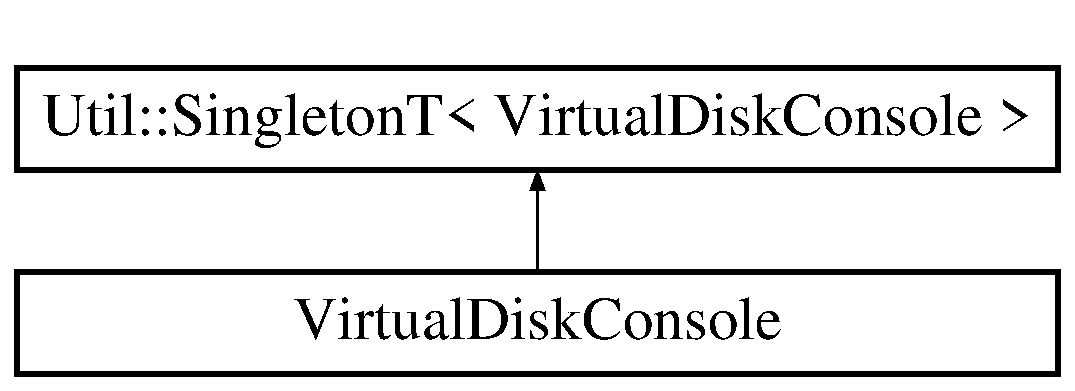
\includegraphics[height=2.000000cm]{class_virtual_disk_console}
\end{center}
\end{figure}
\subsection*{Public 成员函数}
\begin{DoxyCompactItemize}
\item 
\hypertarget{class_virtual_disk_console_aa17d7576f37de378044f9f9c93151300}{void {\bfseries Init} (void)}\label{class_virtual_disk_console_aa17d7576f37de378044f9f9c93151300}

\item 
\hypertarget{class_virtual_disk_console_a96b0c1db50820d232752237bd88d39e0}{void {\bfseries Destroy} (void)}\label{class_virtual_disk_console_a96b0c1db50820d232752237bd88d39e0}

\item 
\hypertarget{class_virtual_disk_console_a95cf6318171081d914394091b115f312}{Util\-::\-String {\bfseries Get\-Curr\-Path} (void) const }\label{class_virtual_disk_console_a95cf6318171081d914394091b115f312}

\item 
\hypertarget{class_virtual_disk_console_ab5f63f91d39a6afc58f34e1688503900}{void {\bfseries Execute\-Command} (const Util\-::\-String \&cmd)}\label{class_virtual_disk_console_ab5f63f91d39a6afc58f34e1688503900}

\item 
\hypertarget{class_virtual_disk_console_a98be6e2fcf8d944977c099a785d884ba}{void {\bfseries Add\-Command} (const Util\-::\-String \&cmd)}\label{class_virtual_disk_console_a98be6e2fcf8d944977c099a785d884ba}

\item 
\hypertarget{class_virtual_disk_console_a63c06c93228aadc734e1370e8efdff37}{void {\bfseries Execute\-Command\-Queue} (void)}\label{class_virtual_disk_console_a63c06c93228aadc734e1370e8efdff37}

\item 
\hypertarget{class_virtual_disk_console_a803b3ac3e53b7f395b662532acb6e98a}{void {\bfseries Print\-Result} (void)}\label{class_virtual_disk_console_a803b3ac3e53b7f395b662532acb6e98a}

\item 
\hypertarget{class_virtual_disk_console_a96890fe0d8cc0176ba0c0558fe75988a}{void {\bfseries Print\-Prompt} (void)}\label{class_virtual_disk_console_a96890fe0d8cc0176ba0c0558fe75988a}

\end{DoxyCompactItemize}
\subsection*{额外继承的成员函数}


\subsection{详细描述}


在文件 Virtual\-Disk\-Console.\-h 第 6 行定义.



该类的文档由以下文件生成\-:\begin{DoxyCompactItemize}
\item 
Virtual\-Disk\-Console/Virtual\-Disk\-Console.\-h\item 
Virtual\-Disk\-Console/Virtual\-Disk\-Console.\-cpp\end{DoxyCompactItemize}

%--- End generated contents ---

% Index
\newpage
\phantomsection
\addcontentsline{toc}{part}{索引}
\printindex

\end{document}
